%%
%% IMWUT submission — single-column manuscript format.
%% Proceedings of the ACM on Interactive, Mobile, Wearable and
%% Ubiquitous Technologies (PACM IMWUT).
%%
%% Submission class options per ACM: `manuscript` (single column, double
%% spaced) + `review` (line numbers for reviewers).  After acceptance, switch
%% to `\documentclass[acmlarge,screen]{acmart}` for the camera-ready.
%%
\documentclass[manuscript,review,screen]{acmart}

\AtBeginDocument{%
  \providecommand\BibTeX{{%
    Bib\TeX}}}

%% Lightweight TODO macro so placeholders are easy to spot in drafts.
%% Removed before the camera-ready.
\usepackage{xcolor}
\newcommand{\todo}[1]{\textcolor{red}{\textbf{[TODO: #1]}}}

%% Figures and graphics.
\usepackage{graphicx}
\graphicspath{{figures/}}

%% TikZ for the S-curve schematic in Background.
\usepackage{tikz}
\usetikzlibrary{decorations.pathreplacing,arrows.meta}

%% Subfigures (used in Background and Evaluation).
\usepackage{subcaption}

%% Side-positioned figures so the Background images sit alongside the prose
%% rather than centred at full width.
\usepackage{wrapfig}

%% Exact figure placement ([H]) for the in-flow pipeline overview in §3.
\usepackage{float}

%% Rights / publication metadata — placeholders, filled in at acceptance.
\setcopyright{acmlicensed}
\copyrightyear{2026}
\acmYear{2026}
\acmDOI{XXXXXXX.XXXXXXX}

%% Journal metadata — IMWUT.
\acmJournal{IMWUT}
\acmVolume{0}
\acmNumber{0}
\acmArticle{0}
\acmMonth{0}

\begin{document}

\title{Smartphone-Only Estimation of Elevator Vertical Displacement
       with Calibrated Confidence Intervals}

\author{Eyal Yakir}
\email{eyalyakir159@gmail.com}
\affiliation{%
  \institution{TBD}
  \city{TBD}
  \country{TBD}
}

\renewcommand{\shortauthors}{Yakir et al.}

\begin{abstract}
  Knowing which floor a smartphone user is on remains an open problem
  on devices that lack a pressure sensor, and the single most common
  floor-change event --- the elevator ride --- is exactly where the
  three workhorses of indoor localisation each break down.
  Pedestrian dead reckoning and step counting estimate horizontal
  trajectory; the cabin removes the steps and the accelerometer
  cannot be integrated vertically without unbounded drift.  Wi-Fi
  fingerprinting demands a per-floor survey, degrades whenever the
  radio environment drifts, and is shielded by the cabin itself.
  Barometric altimetry resolves a floor in principle but assumes a
  pressure sensor that entry-level phones omit, and demands
  re-referencing against weather drift on phones that carry one.

  We present a smartphone-only pipeline that estimates the signed
  vertical displacement~$\Delta h$ of every elevator ride a user
  takes and attaches a calibrated $90\,\%$ confidence interval to
  it, using the phone's accelerometer alone.  The pipeline rests on
  one observation.  The mechanical limits of an elevator cabin force
  the gravity-removed acceleration trace a phone records during a
  ride into a small parametric family of basis functions.  We
  decompose every candidate ride against this family in two stages
  --- segmentation of hours-long inertial streams into discrete
  \texttt{up}\,/\,\texttt{down} ride intervals, and per-ride
  prediction of~$\Delta h$ with a per-ride uncertainty.  Each
  interval is distribution-free with finite-sample coverage
  guarantees, adapts to ride duration, gravity-vector stability, and
  fit quality, and remains valid under both white sensor noise and
  the coloured (drift- and vibration-driven) noise that dominates
  real hand-held recordings.

  We evaluate on \todo{150} experiments spanning \todo{TBD} elevators
  in \todo{TBD} buildings (residential, office, hotel), with a strict
  held-out blind test.  Median CI half-width on the held-out test
  stays below \todo{$\pm 0.9$\,m} on short rides at $90\,\%$
  coverage, an improvement of \todo{TBD\,\%} over the dataset's prior
  best.  We open-source the pipeline, dataset, and evaluation
  harness.
\end{abstract}

\begin{CCSXML}
<ccs2012>
 <concept>
  <concept_id>10003120.10003138.10003140</concept_id>
  <concept_desc>Human-centered computing~Ubiquitous and mobile computing</concept_desc>
  <concept_significance>500</concept_significance>
 </concept>
 <concept>
  <concept_id>10010147.10010178.10010224.10010225</concept_id>
  <concept_desc>Computing methodologies~Sensor data processing</concept_desc>
  <concept_significance>300</concept_significance>
 </concept>
</ccs2012>
\end{CCSXML}

\ccsdesc[500]{Human-centered computing~Ubiquitous and mobile computing}
\ccsdesc[300]{Computing methodologies~Sensor data processing}

\keywords{smartphone sensing, inertial measurement, elevator,
          vertical localization, conformal prediction,
          uncertainty quantification, indoor positioning,
          matched filter}

\maketitle

\section{Introduction}
\label{sec:intro}

% Stakes: who suffers, why the domain matters.
Indoor location services place a smartphone within metres of the right
room on the horizontal plane, using Wi-Fi fingerprinting, BLE beacons,
and visual pedestrian dead reckoning~\cite{liu2007indoor}.  The
vertical axis lags behind.  Knowing the user's floor matters for
emergency dispatch, which routes responders to a floor rather than to
a building entrance.  It matters for venue-aware advertising and
indoor delivery in malls and office towers, and for augmented-reality
experiences anchored to a specific floor of a museum or conference
centre.

% Problem gap: structural limitations, numbered.
Three structural limitations make floor estimation harder than its
horizontal sibling.  \emph{(i)}~Step counting and pedestrian dead
reckoning estimate horizontal trajectory and report nothing about
height~\cite{harle2013pdr}.  \emph{(ii)}~Wi-Fi fingerprinting separates
floors only where the survey covered every floor and the radio
environment has not drifted since~\cite{bahl2000radar}.
\emph{(iii)}~Barometric altimetry resolves a floor in principle, but
the pressure sensor is absent on entry-level phones and demands
re-referencing against weather drift on phones that carry
one~\cite{muralidharan2014barometer}.  The single most common floor-change event
--- the elevator ride --- sits in the regime where every
horizontal-localisation signal degrades at once.

% Insight: kinematic family, no S-curve mechanics, deferred to background.
Elevators are not arbitrary motion.  We found that the mechanical
limits of the cabin force the gravity-removed acceleration trace a
phone records during a ride into a small parametric family of
expected functions.  Section~\ref{sec:background} characterises this
family precisely; what matters in the introduction is that the family
is small enough to enumerate and structured enough to fit a candidate
ride against.  Every claim in this paper rests on it.

% The goal: per-ride displacement with a calibrated interval.
The family turns a hard goal into a tractable one.  Given an inertial
recording of a single elevator ride, we recover the ride's signed
vertical displacement~$\Delta h$ together with a calibrated $90\,\%$
confidence interval.  Recovery reduces to fitting a candidate ride
against the family, which converts a smartphone into a per-ride
vertical-displacement sensor that needs no barometer at inference
time, no Wi-Fi survey, and no per-building calibration.

% Design intuition (Move 4): pipeline shape, no algorithmic detail.
Our pipeline has two stages.  Segmentation extracts ride intervals
from a continuous, possibly hours-long, inertial stream.  Prediction
returns~$\Delta h$ for each interval together with a per-ride
uncertainty.  Both stages read the phone's accelerometer alone.  The
per-ride confidence interval is distribution-free, carries
finite-sample coverage guarantees, and remains valid under both
white sensor noise and the coloured (drift- and vibration-driven)
noise that dominates real hand-held recordings.

% Results preview (Move 6).
We evaluate on \todo{150} experiments spanning \todo{TBD} elevators
across \todo{TBD} buildings (residential, office, hotel), with a
strict held-out blind test.  The system retains its nominal
$90\,\%$ coverage on the blind test.  The median CI half-width
stays below~\todo{$\pm 0.9$\,m} on short rides, and per-bin error
improves on the dataset's prior best by~\todo{TBD\,\%}.
Section~\ref{sec:evaluation} reports the full coverage and error
statistics.

\paragraph{Contributions.}
\begin{enumerate}
  \item \textbf{Per-ride displacement with calibrated coverage.}
    We deliver $90\,\%$, distribution-free, finite-sample confidence
    intervals on~$\Delta h$ from accelerometer data alone, valid
    under both white sensor noise and the coloured noise that
    dominates hand-held recordings.
  \item \textbf{Family-of-basis-functions framework.} We
    characterise the family of expected gravity-removed acceleration
    traces for an elevator ride from the cabin's mechanical limits,
    and use the same family as the substrate for both segmentation
    and per-ride prediction.
  \item \textbf{Dataset and harness.} We release the multi-building
    dataset (\todo{150} experiments, multiple phones per ride,
    barometer ground-truth pipeline), the full evaluation harness,
    and the operator UI used to triage rides.
\end{enumerate}

\paragraph{Roadmap.}
Section~\ref{sec:background} characterises the elevator's mechanical
structure, the physical limits it imposes on a ride, and the family
of expected acceleration functions those limits force.
Section~\ref{sec:algorithm} presents the two-stage algorithm: it
segments an inertial stream into rides and predicts each ride's
$\Delta h$ with a calibrated interval.  Section~\ref{sec:dataset}
describes the dataset and its ground truth, and
Section~\ref{sec:evaluation} reports the train/test split and the
results.  Sections~\ref{sec:discussion} and~\ref{sec:conclusion}
discuss limitations and conclude.

\section{Background: Elevator Kinematics}
\label{sec:background}

This section derives the family of acceleration functions an elevator
ride can produce on a smartphone.  We start from the cabin's mechanical
parts and the physical constraints they impose
(\S\ref{sec:bg-mechanics}), translate those constraints into bounds on
jerk, acceleration, and velocity (\S\ref{sec:bg-bounds}), and then
write down the seven-segment S-curve that the bounds force every ride
to follow (\S\ref{sec:bg-scurve}).  We close with the closed-form
relations between machine parameters and the time constants of the
ride (\S\ref{sec:bg-time-constants}) and the parametric family that
this paper's segmentation and prediction stages
fit~(\S\ref{sec:bg-family}); the heavy algebra lives in
Appendix~\ref{app:derivations}.

\subsection{How a passenger elevator works}
\label{sec:bg-mechanics}

\begin{wrapfigure}{r}{0.34\linewidth}
  \vspace{-0.6em}
  \centering
  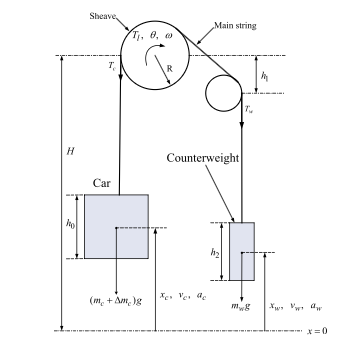
\includegraphics[width=\linewidth]{elevator_schematic.png}
  \caption{A traction elevator at a glance.  A sheave of radius~$R$
    couples the car~($m_c\!+\!\Delta m_c$) to a counterweight
    ($m_w$).  The motor delivers torque~$T_j$ at angular
    velocity~$\omega$; rope tensions $T_v$ and $T_w$ load the
    sheave.  $H$ is the hoistway height; $h_0$ and $h_2$ are the
    cabin and counterweight heights; $h_1$ is the headroom budget
    above the sheave that the brake must respect.}
  \label{fig:elevator-schematic}
  \vspace{-0.5em}
\end{wrapfigure}

A passenger elevator is, mechanically, a single moving piece: a
cabin (the \emph{car}) hanging on a steel rope that runs up over a
sheave at the top of the shaft and down the other side to a
counterweight (Figure~\ref{fig:elevator-schematic}).  A motor turns
the sheave; the cabin and counterweight rise and fall in opposite
directions.  The counterweight is sized to match the empty car
plus roughly half the rated payload, so the motor only has to
drive the small mass difference and the inertia of the moving
parts.  A brake clamps the sheave shaft whenever the motor is
unpowered or anything goes wrong.  Three machine pieces decide how
the cabin can move: the rope (it stretches), the motor (it has a
torque ceiling), and the brake (it has a maximum stopping
distance fixed by the headroom~$h_1$).  The next subsection
turns each into a hard limit on the cabin's motion.

\subsection{Physical limitations and what they bound}
\label{sec:bg-bounds}

Four mechanical realities turn into four hard limits on the cabin's
motion.  Each is the source of one of the parameters our pipeline
fits.

\paragraph{The rope sets the maximum jerk.}
The main rope stretches.  If the motor changes torque too quickly,
the cabin starts to bounce on the rope: the passenger feels it as
a thump, and the rope itself fatigues over time.  Drive
controllers therefore ramp torque through a slew-rate
limit~\cite{macfarlane2003jerk}.  Slew-rate-limiting the torque
is the same as putting a ceiling on the jerk $\dddot h$ the cabin
feels.  The ride-comfort standard ISO~$18738$ pins this at
$j_{\max}\!\approx\!1.0$--$1.6$\,m/s$^3$ for passenger
elevators~\cite{iso18738}.

\paragraph{The motor sets the maximum acceleration.}
At constant velocity the motor only has to fight friction and the
small mass mismatch between cabin and counterweight.  When it
accelerates, it has to push the entire moving mass.  The motor has
a torque ceiling, so cabin acceleration is also capped:
$a_{\max}\!\approx\!0.8$--$1.5$\,m/s$^2$ on commercial traction
elevators.  Older geared machines sit at the low end; newer
gearless ones at the high end.

\paragraph{The brake sets the maximum cruise velocity.}
If anything goes wrong --- a slack rope, an overspeed sensor trip,
loss of power --- the cabin has to stop before it hits the top of
the shaft.  The brake decelerates the cabin at some rate
$a_{\text{brake}}$ and has at most the headroom~$h_1$ above the top
floor to do it in.  Energy says $v_{\max}^{2}\le 2\,a_{\text{brake}}\,h_1$,
which in practice limits cruise velocity to
$v_{\max}\!\approx\!1.0$--$2.5$\,m/s in low- and mid-rise
buildings (CIBSE Guide~D~\cite{cibseguidd2020}).  Faster cabins
exist in skyscrapers, but they require taller headroom and
shaft-mounted buffers.

\paragraph{Only the height changes from ride to ride.}
Once the elevator is built, $j_{\max}$, $a_{\max}$, and $v_{\max}$
are fixed for the building --- often fixed for the manufacturer
and service class.  The only thing that changes ride to ride is
the floor-to-floor height the cabin has to cover, which we
write~$H$ (metres, signed for direction).  Putting the three
limits together, the cabin obeys
\begin{equation}
  \big|\dddot h(t)\big|\le j_{\max},\qquad
  \big|\ddot  h(t)\big|\le a_{\max},\qquad
  \big|\dot   h(t)\big|\le v_{\max},
  \label{eq:elevator-bounds}
\end{equation}
where $\ddot h\!=\!a$ is the gravity-removed vertical acceleration
the phone measures.

\subsection{Why the ride is an S-curve}
\label{sec:bg-scurve}

\paragraph{The optimisation problem.}
The drive solves a simple problem: move the cabin~$H$ metres,
starting and ending at rest, in the shortest possible time, without
ever breaking the three limits in~\eqref{eq:elevator-bounds}.
Write the cabin's altitude as~$h(t)$, its velocity as
$v(t)\!=\!\dot h(t)$, its acceleration as $a(t)\!=\!\ddot h(t)$,
and the controller's command as the jerk $j(t)\!=\!\dddot h(t)$.
The controller picks~$j(t)$; everything else follows by
integration.  Formally we solve
\begin{equation}
  \label{eq:elevator-opt}
  \begin{aligned}
    \underset{T,\,j(\cdot)}{\text{minimize}}\quad
      & T \\[3pt]
    \text{subject to}\quad
      & h(0)=0,\quad h(T)=H,\quad v(0)=v(T)=0, \\
      & |j(t)|\le j_{\max},\quad
        |a(t)|\le a_{\max},\quad
        |v(t)|\le v_{\max}, \\
      & \forall\,t\in[0,T].
  \end{aligned}
\end{equation}

\paragraph{The result.}
Pontryagin's maximum principle, applied
to~\eqref{eq:elevator-opt}, forces the optimal command to be
\emph{bang-bang} on the highest-derivative input.  At every
instant, the optimal jerk takes only three values,
\begin{equation}
  j^{*}(t)\;\in\;\{-j_{\max},\,0,\,+j_{\max}\},
  \label{eq:bang-bang}
\end{equation}
with $j^{*}\!=\!0$ holding the cabin against $|a|\!=\!a_{\max}$ or
$|v|\!=\!v_{\max}$ when one of the lower-order limits is itself
saturated.  Intuitively, any moment spent at an interior value
$|j|<j_{\max}$ is wasted: the cabin could have been pushing
harder and finished sooner.  Appendix~\ref{app:bangbang} sketches
the derivation; we use~\eqref{eq:bang-bang} below.


\paragraph{The S-curve and its three regimes.}
Stitching the bang-bang jerk command~\eqref{eq:bang-bang} together
with the three limits yields the canonical \emph{S-curve}
acceleration profile.  The floor-to-floor height~$H$ alone fixes
how many of the limits a ride saturates, and so splits every ride
into one of three regimes --- long, medium, or short --- shown
side by side in Figure~\ref{fig:scurve-durations}.

\newcommand{\scurvepanel}[5]{%
  % #1 = Tj, #2 = Ta, #3 = Tv, #4 = a_peak (<= amax), #5 = amax (for axis label)
  \begin{tikzpicture}[>=Stealth, font=\scriptsize, scale=0.55]
    \pgfmathsetmacro{\Tj}{#1}
    \pgfmathsetmacro{\Ta}{#2}
    \pgfmathsetmacro{\Tv}{#3}
    \pgfmathsetmacro{\apk}{#4}
    \pgfmathsetmacro{\amx}{#5}
    \pgfmathsetmacro{\Tend}{4*\Tj + 2*\Ta + \Tv}
    \pgfmathsetmacro{\tA}{\Tj}
    \pgfmathsetmacro{\tB}{\Tj+\Ta}
    \pgfmathsetmacro{\tC}{2*\Tj+\Ta}
    \pgfmathsetmacro{\tD}{2*\Tj+\Ta+\Tv}
    \pgfmathsetmacro{\tE}{3*\Tj+\Ta+\Tv}
    \pgfmathsetmacro{\tF}{3*\Tj+2*\Ta+\Tv}
    \pgfmathsetmacro{\tG}{4*\Tj+2*\Ta+\Tv}
    \draw[->] (0,-1.5*\amx) -- (0,1.6*\amx) node[above] {$a(t)$};
    \draw[->] (-0.2,0) -- ({\Tend+0.4},0) node[right] {$t$};
    \draw[dashed,gray!60] (0,{\amx}) -- ({\Tend},{\amx});
    \draw[dashed,gray!60] (0,{-\amx}) -- ({\Tend},{-\amx});
    \node[left,font=\tiny] at (0,{\amx}) {$+a_{\max}$};
    \node[left,font=\tiny] at (0,{-\amx}) {$-a_{\max}$};
    \draw[very thick, blue!70!black]
      (0,0) --
      ({\tA},{\apk}) --
      ({\tB},{\apk}) --
      ({\tC},0) --
      ({\tD},0) --
      ({\tE},{-\apk}) --
      ({\tF},{-\apk}) --
      ({\tG},0);
  \end{tikzpicture}%
}

\begin{figure}[ht]
\centering
% One row per regime: acceleration profile (left) paired with its
% defining time-constant condition and a one-line explanation (right).
\begin{minipage}[c]{0.36\linewidth}\centering
  \scurvepanel{0.6}{0.6}{2.4}{1.0}{1.0}
\end{minipage}\hfill
\begin{minipage}[c]{0.60\linewidth}
  \textbf{Long ride --- 7 segments.}\\
  $T_v>0,\quad T_a>0$\\
  All three limits saturate; a flat $v_{\max}$ cruise splits the
  two trapezoidal lobes.
\end{minipage}

\vspace{1.2em}
\begin{minipage}[c]{0.36\linewidth}\centering
  \scurvepanel{0.6}{0.6}{0.0}{1.0}{1.0}
\end{minipage}\hfill
\begin{minipage}[c]{0.60\linewidth}
  \textbf{Medium ride --- 5 segments.}\\
  $T_v=0,\quad T_a>0$\\
  Jerk and acceleration saturate but the cabin never reaches
  $v_{\max}$; the two lobes touch at the peak-velocity instant.
\end{minipage}

\vspace{1.2em}
\begin{minipage}[c]{0.36\linewidth}\centering
  \scurvepanel{0.5}{0.0}{0.0}{0.55}{1.0}
\end{minipage}\hfill
\begin{minipage}[c]{0.60\linewidth}
  \textbf{Short ride --- 3 segments.}\\
  $T_v=T_a=0$\\
  Only jerk saturates; the two lobes are triangles that meet, with
  peak $|a|<a_{\max}$.
\end{minipage}

\caption{The three S-curve regimes of the time-optimal acceleration
  profile~$a(t)$, all produced by the bang-bang jerk
  command~\eqref{eq:bang-bang} and selected by the floor-to-floor
  height~$H$.  Each row pairs the profile with the time-constant
  condition that defines its regime; longer~$H$ saturates more
  limits.  Closed forms for $T_j$, $T_a$, and~$T_v$ follow
  in~\S\ref{sec:bg-time-constants}.}
\label{fig:scurve-durations}
\end{figure}

\subsection{From machine parameters to ride-time constants}
\label{sec:bg-time-constants}

The bang-bang structure pins every phase of the ride to a
closed-form duration in the machine parameters and the
floor-to-floor height~$H$.  Three durations describe any ride:
\begin{align}
  T_j &= \frac{a_{\max}}{j_{\max}}, \label{eq:Tj}\\
  T_a &= \max\!\left(0,\;\frac{v_{\max}}{a_{\max}}-T_j\right),
         \label{eq:Ta}\\
  T_v &= \max\!\left(0,\;\frac{H}{v_{\max}}-2T_j-T_a\right),
         \label{eq:Tv}
\end{align}
and they sum over the seven phases to the total ride duration
\begin{equation}
  T_{\text{ride}} \;=\; 4T_j + 2T_a + T_v
  \;=\; \frac{H}{v_{\max}} + \frac{v_{\max}}{a_{\max}}
        + \frac{a_{\max}}{j_{\max}}
  \quad\text{(trapezoidal regime).}
  \label{eq:elevator-durations}
\end{equation}

\begin{wrapfigure}{r}{0.46\linewidth}
  \vspace{-0.6em}
  \centering
  \resizebox{\linewidth}{!}{%
  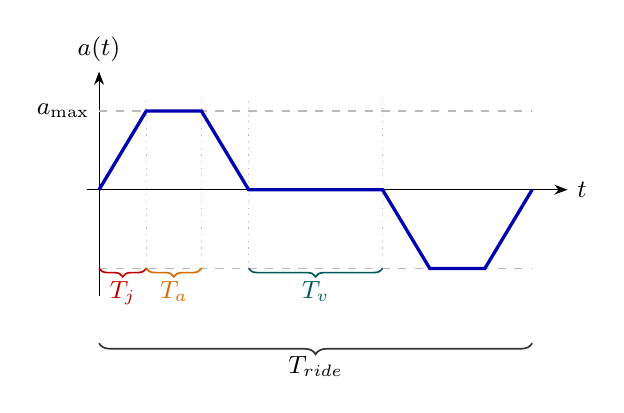
\begin{tikzpicture}[>=Stealth, font=\small]
    \pgfmathsetmacro{\Tj}{0.6}
    \pgfmathsetmacro{\Ta}{0.7}
    \pgfmathsetmacro{\Tv}{1.7}
    \pgfmathsetmacro{\amax}{1.0}
    \pgfmathsetmacro{\Tend}{4*\Tj+2*\Ta+\Tv}
    \pgfmathsetmacro{\tA}{\Tj}
    \pgfmathsetmacro{\tB}{\Tj+\Ta}
    \pgfmathsetmacro{\tC}{2*\Tj+\Ta}
    \pgfmathsetmacro{\tD}{2*\Tj+\Ta+\Tv}
    \pgfmathsetmacro{\tE}{3*\Tj+\Ta+\Tv}
    \pgfmathsetmacro{\tF}{3*\Tj+2*\Ta+\Tv}
    \pgfmathsetmacro{\tG}{4*\Tj+2*\Ta+\Tv}
    \draw[->] (0,-1.35) -- (0,1.5) node[above] {$a(t)$};
    \draw[->] (-0.15,0) -- ({\Tend+0.45},0) node[right] {$t$};
    \draw[dashed,gray!55] (0,\amax) -- (\Tend,\amax);
    \draw[dashed,gray!55] (0,-\amax) -- (\Tend,-\amax);
    \node[left] at (0,\amax) {$a_{\max}$};
    \foreach \tt in {\tA,\tB,\tC,\tD}
      \draw[dotted,gray!55] (\tt,-1.0) -- (\tt,1.15);
    \draw[very thick,blue!70!black]
      (0,0) -- (\tA,\amax) -- (\tB,\amax) -- (\tC,0)
      -- (\tD,0) -- (\tE,-\amax) -- (\tF,-\amax) -- (\tG,0);
    \draw[decorate,decoration={brace,amplitude=3pt,mirror},semithick,red!75!black]
      (0,-1.0) -- (\tA,-1.0) node[midway,below=1pt,red!75!black] {$T_j$};
    \draw[decorate,decoration={brace,amplitude=3pt,mirror},semithick,orange!85!black]
      (\tA,-1.0) -- (\tB,-1.0) node[midway,below=1pt,orange!85!black] {$T_a$};
    \draw[decorate,decoration={brace,amplitude=3pt,mirror},semithick,teal!70!black]
      (\tC,-1.0) -- (\tD,-1.0) node[midway,below=1pt,teal!70!black] {$T_v$};
    \draw[decorate,decoration={brace,amplitude=4pt,mirror},semithick,black!80]
      (0,-1.95) -- (\tG,-1.95) node[midway,below=1pt,black] {$T_{\text{ride}}$};
  \end{tikzpicture}}
  \caption{The four ride-time constants on the acceleration
    trace~$a(t)$ of a trapezoidal ride: jerk ramp~$T_j$, the
    $a_{\max}$ plateau~$T_a$, the $v_{\max}$ cruise~$T_v$ (the
    flat $a\!=\!0$ gap between lobes), and the total
    ride~$T_{\text{ride}}$.}
  \label{fig:ride-time-constants}
  \vspace{-0.5em}
\end{wrapfigure}
Figure~\ref{fig:ride-time-constants} locates the four durations on
a single ride.  The jerk ramp~$T_j$ and the acceleration
plateau~$T_a$ are constants of the building.  $T_j$ depends only on
the machine --- about $0.77$\,s for a typical lift
($a_{\max}\!=\!1.0$\,m/s$^2$, $j_{\max}\!=\!1.3$\,m/s$^3$) --- and
$T_a$ vanishes on rides too short to reach~$v_{\max}$.  Only the
cruise~$T_v$ scales with ride length, growing as~$H/v_{\max}$.
Equation~\eqref{eq:elevator-durations} is the inversion handle
later sections use to recover~$H$ jointly with the machine
parameters; Appendix~\ref{app:derivations} derives all four
constants from the bounds in~\eqref{eq:elevator-bounds}.

\subsection{The trapezoid basis function and the parametric family}
\label{sec:bg-family}

Combining \eqref{eq:elevator-bounds}--\eqref{eq:elevator-durations},
every ride is fixed by four parameters,
\begin{equation}
  \boxed{\theta \;=\; (j_{\max},\, a_{\max},\, v_{\max},\, H)},
  \label{eq:elevator-params}
\end{equation}
three constants of the building and the ride-specific height~$H$.

\paragraph{The trapezoid basis function.}
Each acceleration lobe of the S-curve is a trapezoid in time --- a
ramp up, a flat top, and a ramp down.  We normalise it to the
trapezoid basis function
\begin{equation}
  \tau_{W,f}(t)=
  \begin{cases}
    1 & |t|\le fW,\\
    \dfrac{W-|t|}{(1-f)\,W} & fW < |t|\le W,\\
    0 & |t|>W,
  \end{cases}
  \label{eq:trap-template}
\end{equation}
of \emph{half-width}~$W$ and \emph{flat fraction}~$f\in[0,1]$: a
unit plateau over $[-fW,fW]$ joined to zero by two linear ramps
(Figure~\ref{fig:trap-template}).

\paragraph{Mapping to the machine parameters.}
The first lobe spans $2T_j+T_a$, so the machine parameters fix
$(W,f)$ exactly:
\begin{align}
  W &= T_j+\tfrac12 T_a
     = \frac{a_{\max}}{2\,j_{\max}}
       +\tfrac12\!\max\!\Big(0,\,\tfrac{v_{\max}}{a_{\max}}-T_j\Big),
     \label{eq:W-from-kinematics}\\
  f &= \frac{T_a}{T_a+2T_j}
     = \frac{\max\!\big(0,\,v_{\max}/a_{\max}-T_j\big)}
            {\max\!\big(0,\,v_{\max}/a_{\max}-T_j\big)+2T_j}.
     \label{eq:f-from-kinematics}
\end{align}
A short hop that never reaches $v_{\max}$ has $T_a\!=\!0$ and
$f\!=\!0$, a pure triangle; a long ride has $T_a\!\gg\!T_j$ and
$f\!\to\!1$, a near-rectangular plateau.  The two lobes pull
apart --- their centroid spacing $\Delta t_c$ exceeds $2W$ ---
only once a $v_{\max}$ cruise opens between them, the 7-segment
regime of~\S\ref{sec:bg-scurve}.

\paragraph{The parametric family.}
Every ride is therefore a pair of opposite-sign trapezoids of
shared shape,
\begin{equation}
  a_\theta(t)
  \;=\; s\,A\,\tau_{W,f}(t-t_{c,1})
        \;-\; s\,A\,\tau_{W,f}(t-t_{c,2}),
  \label{eq:ride-template}
\end{equation}
with amplitude $A\!=\!a_{\max}$, direction $s\!\in\!\{+1,-1\}$, and
centroid spacing $\Delta t_c\!=\!t_{c,2}-t_{c,1}\!=\!H/v_{\max}$
(Appendix~\ref{app:derivations}).

\begin{wrapfigure}{r}{0.42\linewidth}
  \vspace{-0.6em}
  \centering
  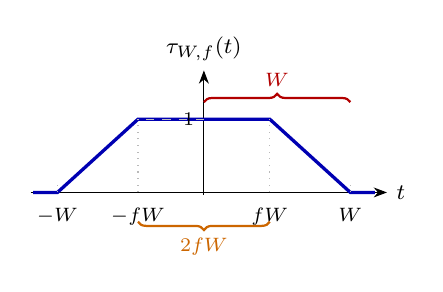
\begin{tikzpicture}[>=Stealth, font=\footnotesize, scale=0.62]
    \pgfmathsetmacro{\W}{3.0}
    \pgfmathsetmacro{\f}{0.45}
    \pgfmathsetmacro{\fW}{\f*\W}
    \pgfmathsetmacro{\hgt}{1.5}
    \draw[->] ({-\W-0.55},0) -- ({\W+0.75},0) node[right] {$t$};
    \draw[->] (0,-0.05) -- (0,{\hgt+1.0}) node[above] {$\tau_{W,f}(t)$};
    \draw[very thick, blue!70!black]
      ({-\W-0.5},0) -- (-\W,0) --
      (-\fW,\hgt) -- (\fW,\hgt) --
      (\W,0) -- ({\W+0.5},0);
    \draw[dashed,gray!50] (0,\hgt) -- (-\fW,\hgt);
    \node[left] at (0,\hgt) {\scriptsize $1$};
    \draw[dotted,gray!55] (-\W,0) -- (-\W,0.15);
    \draw[dotted,gray!55] (-\fW,0) -- (-\fW,\hgt);
    \draw[dotted,gray!55] (\fW,0) -- (\fW,\hgt);
    \draw[dotted,gray!55] (\W,0) -- (\W,0.15);
    \node[below=2pt] at (-\W,0)  {\scriptsize $-W$};
    \node[below=2pt] at (-\fW,0) {\scriptsize $-fW$};
    \node[below=2pt] at (\fW,0)  {\scriptsize $fW$};
    \node[below=2pt] at (\W,0)   {\scriptsize $W$};
    \draw[decorate,decoration={brace,amplitude=3pt},thick,red!70!black]
      (0,{\hgt+0.35}) -- (\W,{\hgt+0.35})
      node[midway,above=2pt,red!70!black] {\scriptsize $W$};
    \draw[decorate,decoration={brace,amplitude=3pt,mirror},thick,orange!80!black]
      (-\fW,-0.6) -- (\fW,-0.6)
      node[midway,below=2pt,orange!80!black] {\scriptsize $2fW$};
  \end{tikzpicture}
  \caption{The trapezoid basis function $\tau_{W,f}(t)$
    of~\eqref{eq:trap-template}.}
  \label{fig:trap-template}
  \vspace{-0.5em}
\end{wrapfigure}
Three facts about this family~$\mathcal{F}_{\text{ride}}$ drive
the rest of the paper.
\emph{(i)}~Three of its parameters are constants of the building, so
a ride differs from the building's other rides only in the
height~$H$ --- the single quantity the predictor of
\S\ref{sec:algorithm} recovers.  \emph{(ii)}~The two lobes carry
equal and opposite area, so
$\int_0^{T_{\text{ride}}}a_\theta(t)\,dt\!=\!0$ --- the zero-mean
anchor for any ZUPT-style predictor.  \emph{(iii)}~The lobe
spacing $\Delta t_c\!=\!H/v_{\max}$ is a scale-free estimator
of~$H$, so the matched-filter detector needs no per-building
amplitude calibration.

\subsection{The smartphone accelerometer}
\label{sec:bg-imu}

\begin{wrapfigure}{r}{0.31\linewidth}
  \vspace{-0.6em}
  \centering
  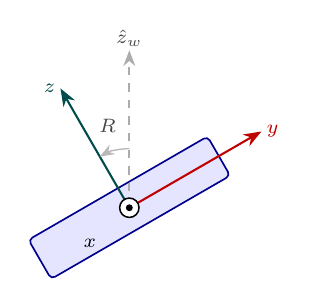
\begin{tikzpicture}[>=Stealth, font=\scriptsize, scale=1.25]
    \draw[rotate=30, rounded corners=1.6pt, line width=0.6pt,
          draw=blue!55!black, fill=blue!10]
          (-1.05,-0.23) rectangle (1.05,0.23);
    \draw[->, dashed, gray!65, line width=0.6pt] (0,0) -- (90:1.6)
          node[above, gray!55!black, inner sep=1pt] {$\hat z_w$};
    \draw[->, red!75!black, line width=0.75pt] (0,0) -- (30:1.55)
          node[right, inner sep=1.5pt] {$y$};
    \draw[->, teal!60!black, line width=0.75pt] (0,0) -- (120:1.4)
          node[left, inner sep=1.5pt] {$z$};
    \draw[fill=white, line width=0.55pt] (0,0) circle (2.8pt);
    \fill (0,0) circle (1pt);
    \node[inner sep=1pt] at (-0.4,-0.36) {$x$};
    \draw[->, gray!55, line width=0.5pt] (90:0.6) arc (90:120:0.6);
    \node[gray!55!black, inner sep=1pt] at (105:0.86) {$R$};
  \end{tikzpicture}
  \caption{Body axes $x,y,z$ tilt from the world
    vertical~$\hat z_w$ by an unknown rotation~$R$.}
  \label{fig:accel-frame}
  \vspace{-0.6em}
\end{wrapfigure}

The pipeline reads a single phone sensor --- the accelerometer ---
and one obstacle separates its raw signal from the vertical
acceleration a ride produces: the phone's unknown orientation.

\paragraph{The accelerometer.}
Every phone carries a six-axis MEMS IMU~\cite{beeby2004mems}.  Its
\texttt{TYPE\_LINEAR\_ACCELERATION} stream reports the
gravity-removed acceleration as a three-vector
$\mathbf{a}=(a_x,a_y,a_z)$ along the phone's \emph{body axes} --- the
$x,y,z$ fixed to the case (Figure~\ref{fig:accel-frame}).  The
sensor-hub rate varies by device, so we resample every recording to
a uniform $100$\,Hz grid ($\Delta t\!=\!10$\,ms).  The noise floor
is white, but a hand-held phone adds coloured drift and
$1\text{--}50$\,Hz vibration, so later sections fit the noise model
on real ride residuals.

\paragraph{The unknown vertical.}
An elevator ride is purely vertical: the cabin accelerates along the
world up-axis~$\hat z_w$, and that one scalar~$a(t)$ is all the
pipeline wants.  The accelerometer, though, measures along the
phone's body axes, and a hand-held phone tilts arbitrarily.  An
unknown rotation~$R$ separates the two frames, so the vertical
signal spreads across all three channels,
$\mathbf{a}=R^{\!\top}\!a\,\hat z_w$ --- the body channel~$a_z$ is
not the world vertical.  Recovering~$a(t)$ means recovering which
body direction points up; the accelerometer-only pipeline reads it
from gravity in the stationary windows around each ride.

In short, the pipeline works from a single $100$\,Hz body-frame
acceleration stream.

\section{Dataset and Ground Truth}
\label{sec:dataset}

The dataset is a field campaign of \todo{$\approx$150} elevator
rides recorded across \todo{7} elevators in \todo{6} buildings in
central Israel (Table~\ref{tab:app-sessions}).  The buildings span
residential, office, and hotel cabins, each with a different cabin
geometry, motor, and floor-to-floor height, so no estimator can
overfit a single machine.  Four phones, carried together, recorded
every ride, so one physical event produced four heterogeneous
accelerometer traces --- different MEMS parts, sampling jitter, and
noise floors.  At least one of the four phones carries a barometric
pressure sensor, which serves as the ground-truth device even when
the phone under test has none.

\begin{wrapfigure}{r}{0.42\linewidth}
  \vspace{-0.7em}
  \centering
  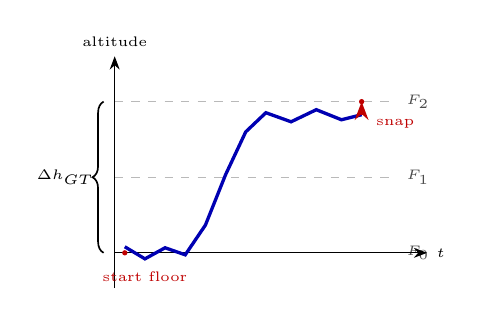
\begin{tikzpicture}[>=Stealth, font=\scriptsize, scale=0.64]
    \foreach \y/\name in {0/{$F_0$}, 1.5/{$F_1$}, 3.0/{$F_2$}}{
      \draw[dashed, gray!55] (0,\y) -- (5.6,\y);
      \node[gray!60!black, right, font=\tiny] at (5.6,\y) {\name};
    }
    \draw[->] (0,-0.7) -- (0,3.9) node[above, font=\tiny] {altitude};
    \draw[->] (0,0) -- (6.2,0) node[right, font=\tiny] {$t$};
    \draw[very thick, blue!70!black]
      (0.2,0.12) -- (0.6,-0.12) -- (1.0,0.10) -- (1.4,-0.04) --
      (1.8,0.55) -- (2.2,1.55) -- (2.6,2.40) -- (3.0,2.78) --
      (3.5,2.60) -- (4.0,2.84) -- (4.5,2.64) -- (4.9,2.74);
    \fill[red!75!black] (0.2,0) circle (1.5pt);
    \node[red!75!black, below, font=\tiny] at (0.6,-0.18) {start floor};
    \draw[->, red!75!black, thick] (4.9,2.74) -- (4.9,3.0);
    \fill[red!75!black] (4.9,3.0) circle (1.5pt);
    \node[red!75!black, right, font=\tiny] at (5.0,2.55) {snap};
    \draw[decorate, decoration={brace, amplitude=4pt}, semithick]
      (-0.22,0) -- (-0.22,3.0)
      node[midway, left, font=\tiny] {$\Delta h_{\text{GT}}$};
  \end{tikzpicture}
  \caption{Snapping the drifting barometer altitude (blue) to the
    nearest \emph{gramushka} floor line (dashed) yields a drift-free
    ground-truth~$\Delta h$.}
  \label{fig:gt-snap}
  \vspace{-0.6em}
\end{wrapfigure}

Every ride's signed displacement~$\Delta h$ comes from the barometer
rather than from hand-labelling.  We invert the pressure stream to
altitude through the ISA barometric formula; a consumer barometer
resolves altitude to roughly $10$\,cm, an order of magnitude finer
than the $\sim\!3$\,m inter-floor pitch the pipeline must separate.
Low-pass filtering and differencing the same altitude trace yields
the \texttt{up}, \texttt{down}, and \texttt{outside} interval labels
that cut each session into discrete rides.  A phone without a
barometer borrows the pressure stream of a co-carried device,
aligned to it by accelerometer cross-correlation
(Appendix~\ref{app:dataset}).

Raw barometric altitude drifts with weather and building airflow, so
we snap it to the building itself.  Each building contributes a
\emph{gramushka} table --- the floor elevations read from its
accordion-folded architectural drawing (Figure~\ref{fig:gt-snap}).
We anchor every session at its known start floor and integrate the
barometer altitude across each detected ride.  Snapping the ride
endpoint to the nearest table floor makes the ground-truth~$\Delta h$
a true floor-to-floor displacement.  The pipeline flags any snap
whose distance exceeds \todo{TBD}\,m for manual review rather than
forcing it, and the one elevator without a drawing falls back to the
drift-corrected barometer~$\Delta h$ (Appendix~\ref{app:dataset}).

\section{Algorithm}
\label{sec:algorithm}

The pipeline converts a continuous, hours-long accelerometer stream
into one signed displacement~$\Delta h$ per elevator ride, each
carrying a calibrated $90\,\%$ confidence interval, in two stages
(Figure~\ref{fig:pipeline}).  Segmentation slices the stream into
discrete ride intervals~(\S\ref{sec:algo-seg}); prediction fits each
interval for its~$\Delta h$ and uncertainty~(\S\ref{sec:algo-pred}).
Both stages reuse the trapezoid family of~\S\ref{sec:bg-family}
directly: a ride is an opposite-sign pair of trapezoid
lobes~\eqref{eq:ride-template}, so the matched filter that finds a
ride is the matched filter that measures it.

\begin{figure}[H]
\centering
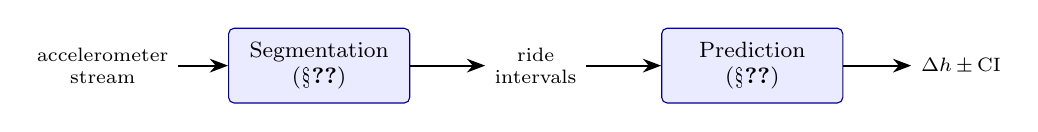
\begin{tikzpicture}[>=Stealth, font=\footnotesize,
    stage/.style={draw, rounded corners=2pt, align=center,
                  inner sep=4pt, minimum width=2.3cm,
                  minimum height=0.95cm, draw=blue!55!black,
                  fill=blue!8},
    data/.style={align=center, font=\scriptsize}]
  \node[data]  (in)    at (0,0)    {accelerometer\\stream};
  \node[stage] (seg)   at (2.75,0) {Segmentation\\(\S\ref{sec:algo-seg})};
  \node[data]  (rides) at (5.5,0)  {ride\\intervals};
  \node[stage] (pred)  at (8.25,0) {Prediction\\(\S\ref{sec:algo-pred})};
  \node[data]  (out)   at (10.9,0) {$\Delta h\,\pm\,$CI};
  \draw[->,line width=0.8pt] (in)    -- (seg);
  \draw[->,line width=0.8pt] (seg)   -- (rides);
  \draw[->,line width=0.8pt] (rides) -- (pred);
  \draw[->,line width=0.8pt] (pred)  -- (out);
\end{tikzpicture}
\caption{The two-stage pipeline.  Segmentation turns a continuous
  accelerometer stream into discrete ride intervals; prediction turns
  each interval into a signed displacement~$\Delta h$ with a
  calibrated confidence interval.  Both stages fit the trapezoid ride
  family of~\S\ref{sec:bg-family}.}
\label{fig:pipeline}
\end{figure}

\subsection{Segmentation}
\label{sec:algo-seg}

Segmentation cuts an hours-long accelerometer stream into discrete
ride intervals, each tagged \texttt{up} or \texttt{down}.  A ride is
an opposite-sign pair of trapezoid lobes~\eqref{eq:ride-template}, so
segmentation detects candidate lobes~(\S\ref{sec:algo-detect}) and
then pairs them into rides~(\S\ref{sec:algo-pair}).

\subsubsection{Detecting candidate lobes}
\label{sec:algo-detect}

The pipeline projects the three-axis accelerometer onto the session's
gravity direction (\S\ref{sec:bg-imu}) and smooths it into a signed
vertical trace~$a(t)$.  A least-squares matched filter scores~$a(t)$
against every lobe template~$\tau_{W,f}$ of the
family~$\mathcal{F}_{\text{ride}}$ (\S\ref{sec:bg-family}): at each
sample~$i$, fitting one amplitude to the length-$2W$
window~$a_{[i]}$ centred on~$i$ gives
\begin{equation}
  \hat A_{W,f}(i)=
    \frac{\langle a_{[i]},\,\tau_{W,f}\rangle}{\|\tau_{W,f}\|^{2}},
  \qquad
  R^{2}_{W,f}(i)=
    1-\frac{\|a_{[i]}-\hat A_{W,f}(i)\,\tau_{W,f}\|^{2}}
           {\|a_{[i]}\|^{2}}.
  \label{eq:matched-filter}
\end{equation}
Collapsing the $(W,f)$ grid by amplitude sign yields, per sample,
\begin{equation}
  R^{2}(i)=\max_{W,f}R^{2}_{W,f}(i),
  \qquad
  R^{2}_{\pm}(i)=\max_{\,\pm\hat A_{W,f}(i)>0}R^{2}_{W,f}(i),
  \label{eq:signed-r2}
\end{equation}
where a high $R^{2}_{+}(i)$ marks a take-off lobe and a high
$R^{2}_{-}(i)$ a landing lobe.  A candidate lobe is a strict local
maximum of $R^{2}_{+}$ or~$R^{2}_{-}$ that clears an amplitude and a
shape floor,
\begin{equation}
  |\hat A(i)|\ge a_{\min},
  \qquad
  R^{2}(i)\ge r_{\min},
  \label{eq:detect-gate}
\end{equation}
with $\hat A(i)$ the amplitude at the best grid cell; non-maximum
suppression then drops near-duplicates within~$\delta_{\mathrm{nms}}$
and keeps same-sign lobes at least~$\Delta_{\mathrm{ss}}$ apart
(Figure~\ref{fig:signed-r2}).  The grid bounds
\eqref{eq:W-from-kinematics}--\eqref{eq:f-from-kinematics} and the
thresholds are calibrated on the training set
(Appendix~\ref{app:segmentation}).

\begin{figure}[H]
\centering
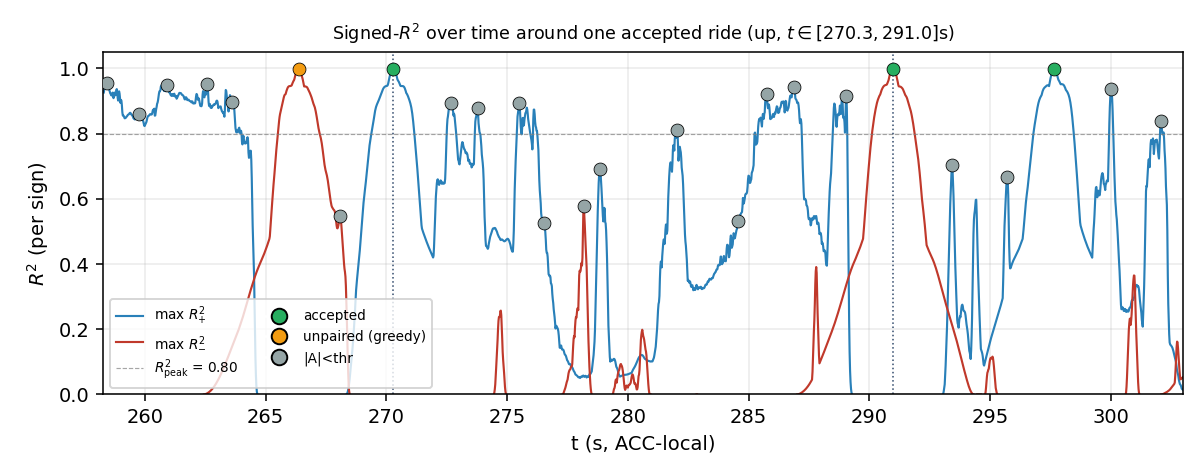
\includegraphics[width=0.7\linewidth]{trapezoid_signed_r2_example.png}
\caption{Signed score traces $R^{2}_{+}(t)$ (take-off, blue) and
  $R^{2}_{-}(t)$ (landing, red) around one ride.  Local maxima are
  candidate lobes; dot colour marks the first stage to reject each
  peak, leaving the committed take-off/landing pair (green).}
\label{fig:signed-r2}
\end{figure}

\subsubsection{Pairing candidate lobes into rides}
\label{sec:algo-pair}

Each candidate lobe~$i$ admits an opposite-sign partner set inside
the ride-duration window,
\begin{equation}
  \mathcal{P}(i)=\bigl\{\,j:\;
    \operatorname{sign}\hat A(j)=-\operatorname{sign}\hat A(i),\;\;
    t_{\min}\le |t_j-t_i|\le t_{\max}\,\bigr\}.
  \label{eq:partner-set}
\end{equation}
A genuine ride's two lobes are cut from one cabin profile, so each
pair $(i,j)$ is fitted with a single template and a single shared
amplitude.  With $a_k$ the $k$th lobe window, $P_k=\|a_k\|^{2}$,
$u_k=s_k\langle a_k,\tau_{W,f}\rangle$ its sign-corrected
correlation, and $N=\|\tau_{W,f}\|^{2}$,
\begin{equation}
  A^{\star}(W,f)=\frac{u_1+u_2}{2N},
  \qquad
  R^{2}_k(W,f)=1-\frac{P_k-2A^{\star}u_k+(A^{\star})^{2}N}{P_k},
  \label{eq:joint-fit}
\end{equation}
and the pair score is
$S(i,j)=\max_{W,f}\tfrac12\bigl(R^{2}_1+R^{2}_2\bigr)$, attained at
$(W^{\star},f^{\star},A^{\star})$.  These starred values describe one
\emph{average} lobe: the fit assumes take-off and landing share a
shape, so $A^{\star}$ averages the two single-lobe amplitudes.  A
high $S$ means both lobes trace out that same trapezoid.  The pair is admissible when
\begin{equation}
  S(i,j)\ge r_{\mathrm{pair}},
  \quad
  A^{\star}\ge a_{\mathrm{pair}},
  \quad
  E(i,j)\ge e_{\min},
  \quad
  \mathrm{RMS}_{\mathrm{mid}}\le \rho\,A^{\star}.
  \label{eq:pair-gate}
\end{equation}
The grid energy~$E$ averages the clamped joint~$R^{2}$ over every
cell of the $(W,f)$ template grid~$G$,
\begin{equation}
  E(i,j)=\frac{1}{|G|}\sum_{(W,f)\in G}
    \max\!\bigl(0,\;\tfrac12(R^{2}_1(W,f)+R^{2}_2(W,f))\bigr),
  \label{eq:grid-energy}
\end{equation}
so a real ride --- which lights a broad band of cells, not one ---
clears the floor~$e_{\min}$.  The cruise term
$\mathrm{RMS}_{\mathrm{mid}}$ is the trace RMS on the inter-lobe
stretch, near zero while the cabin holds constant velocity.  A greedy
resolver ranks admissible pairs by
\begin{equation}
  \operatorname{rank}(i,j)=S(i,j)-\lambda\,|t_j-t_i|
  \label{eq:pair-rank}
\end{equation}
and commits them highest-first, skipping any that reuse a lobe or
overlap a committed interval.  The penalty~$\lambda$ defeats the
\emph{super pair} --- a take-off matched to a far-later landing,
which scores like a true ride but spans far longer.  The committed
pairs are the ride intervals passed to prediction.

\begin{center}
\textcolor{blue}{\bfseries Appendix~\ref{app:thresholds} explains and
illustrates every detection and pair-filter threshold.}
\end{center}

\subsection{Prediction}
\label{sec:algo-pred}

Prediction takes one ride interval and returns the signed
displacement~$\Delta h$, a per-ride standard deviation~$\sigma$, a
calibrated $90\,\%$ confidence interval, and an \texttt{accepted}
flag.  Displacement follows from one fact: an accelerometer measures
acceleration, and displacement is its double integral --- integrate
the vertical trace~$a(t)$ once for velocity, twice for~$\Delta h$.
The front end recovers that signed vertical trace from the three-axis
accelerometer by the gravity projection of~\S\ref{sec:bg-imu}.

Two accelerometer-only algorithms run that double integral by
different routes.  ZUPT double integration~(\S\ref{sec:algo-zupt})
integrates the measured~$a(t)$ directly, anchored by the cabin
resting at both ends of the ride.  The trapezoid pulse-pair
fit~(\S\ref{sec:algo-trapezoid}) integrates a model instead: it
constructs the ride's theoretical acceleration signal --- the
trapezoid pulse pair of~\S\ref{sec:bg-family} --- and integrates it
in closed form, reading~$\Delta h$ off a formula in the fitted shape.
Section~\ref{sec:evaluation} compares them head to head.

Both feed three shared stages: a per-ride error
model~(\S\ref{sec:algo-error}), a conformal layer that
calibrates~$\sigma$ into the interval~(\S\ref{sec:algo-ci}), and a
quality filter that sets the \texttt{accepted}
flag~(\S\ref{sec:algo-quality}).  The trapezoid fit borrows only
ZUPT's cruise-velocity scale as an amplitude anchor, never its
displacement, so the two stay independent estimators and the
comparison of~\S\ref{sec:evaluation} stays meaningful.

\subsubsection{ZUPT double integration}
\label{sec:algo-zupt}

ZUPT recovers~$\Delta h$ by double-integrating the measured vertical
acceleration under a zero-velocity boundary at both ends of the ride,
\begin{equation}
  v(t)=\int_{0}^{t}\!a(\tau)\,d\tau
        \;-\;\frac{t}{T}\int_{0}^{T}\!a(\tau)\,d\tau,
  \qquad
  \Delta h=\int_{0}^{T}\!v(t)\,dt,
  \label{eq:zupt-integral}
\end{equation}
over a ride of duration~$T$.

The boundary assumption anchors the integral.  A ride begins and ends
with the cabin at rest, so $v(0)=v(T)=0$.  The first integral
of~\eqref{eq:zupt-integral} enforces $v(0)=0$ by construction; the
linear ramp term subtracts the integrated-noise drift that would
otherwise leave $v(T)\neq0$ --- the zero-velocity update that names
the method.

ZUPT integrates only the moving span: the pipeline thresholds the
vertical trace at $|a(t)|=0.10\,\mathrm{m/s^2}$ and zeroes the quiet
pre- and post-roll, so noise outside the ride never enters the
integral.  The count~$N$ of active samples sets the scale of the
error model~(\S\ref{sec:algo-error}).

\subsubsection{Trapezoid pulse-pair fit}
\label{sec:algo-trapezoid}

\begin{wrapfigure}{r}{0.40\linewidth}
  \vspace{-0.7em}
  \centering
  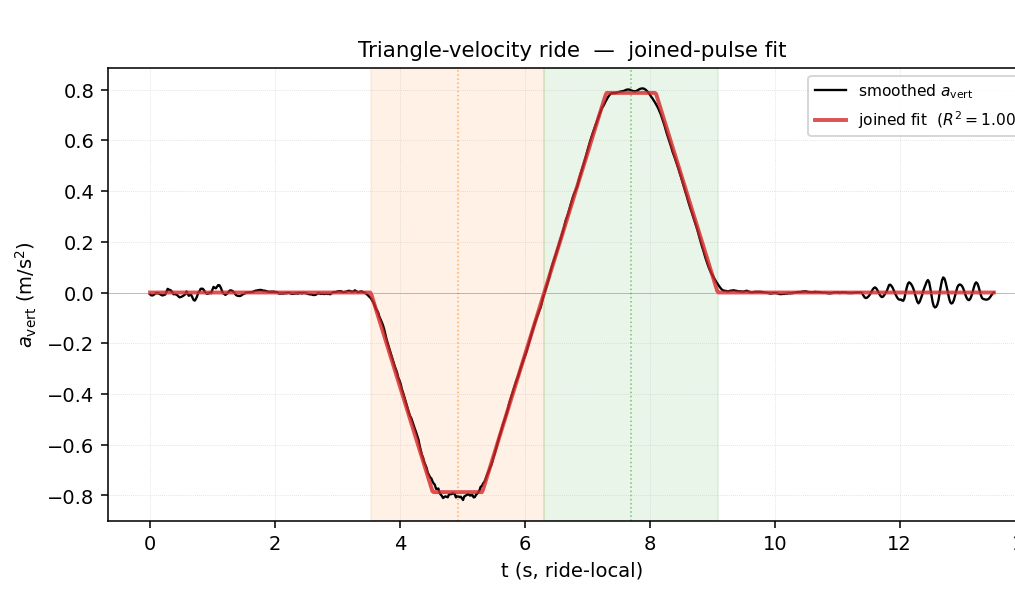
\includegraphics[width=\linewidth]{trapezoid_pulse_pair.png}
  \caption{The reconstructed signal~$a_\theta(t)$ (red) overlaid on
    the smoothed vertical trace (black) for one ride: two
    opposite-sign trapezoid lobes centred at~$t_{c,1}$
    and~$t_{c,2}$.}
  \label{fig:trap-pulse-pair}
  \vspace{-0.6em}
\end{wrapfigure}

The trapezoid fit recovers~$\Delta h$ from the \emph{shape} of the
acceleration trace.  The ride's theoretical signal is the S-curve
of~\S\ref{sec:bg-scurve}, set by three machine
parameters~$(j_{\max},a_{\max},v_{\max})$ besides the height.  Fitting
all three to a hand-held recording is ill-conditioned: the jerk ramps
occupy too small a fraction of the ride to constrain them.  The fit
instead collapses each acceleration lobe to the trapezoid~$\tau_{W,f}$
the detector already uses, a two-parameter shape the bang-bang jerk
command makes exact~(\S\ref{sec:bg-family}).

The segmenter (\S\ref{sec:algo-pair}) already returns the fitted
parameters~$(W,f,A,s,t_{c,1},t_{c,2})$ that reconstruct the ride's
acceleration as the opposite-sign trapezoid pair
\begin{equation}
  a_\theta(t) \;=\; sA\,\tau_{W,f}(t-t_{c,1})
                 \;-\; sA\,\tau_{W,f}(t-t_{c,2}),
  \label{eq:trap-signal}
\end{equation}
the estimated ride signal (Figure~\ref{fig:trap-pulse-pair}).
Double-integrating~$a_\theta(t)$ gives~$\Delta h$ in closed form,
\begin{equation}
  \Delta h \;=\; s\,A\,W\,(1+f)\,\Delta t_c,
  \qquad \Delta t_c=t_{c,2}-t_{c,1};
  \label{eq:dh-closed}
\end{equation}
Appendix~\ref{app:prediction} works through the integral and the
joined-pulse limit.

\subsubsection{Theoretical error analysis}
\label{sec:algo-error}

Every prediction carries a per-ride standard deviation~$\sigma$
derived from its own fit, not a constant.  The two algorithms reach
that~$\sigma$ from different error sources.

\paragraph{ZUPT.}
Double integration accumulates sensor noise.  Integrating white noise
of standard deviation~$\sigma_a$ twice over~$N$ active samples of
spacing~$\Delta t$ gives an end-point displacement variance whose
root is
\begin{equation}
  \sigma_{\mathrm{white}}
   \;=\; \sigma_a\,\Delta t^{2}\,\sqrt{N^{3}/12},
  \label{eq:sigma-zupt}
\end{equation}
the classic ZUPT result, with the factor~$1/12$ crediting the linear
drift correction of~\eqref{eq:zupt-integral} for removing one degree
of freedom.  A hand-held phone carries three further error sources,
which the total budget adds to the white-noise term in quadrature,
\begin{equation}
  \sigma_{\mathrm{ZUPT}}^{2}
   \;=\;\sigma_{\mathrm{white}}^{2}
        +\sigma_{\mathrm{mech}}^{2}
        +\sigma_{\mathrm{rel}}^{2}
        +\sigma_{\mathrm{proj}}^{2}\,:
  \label{eq:sigma-zupt-total}
\end{equation}
a mechanical-jitter term~$\sigma_{\mathrm{mech}}$ for hand and pocket
movement, a relative-scale term~$\sigma_{\mathrm{rel}}$ that grows
with~$|\Delta h|$, and a projection penalty~$\sigma_{\mathrm{proj}}$
for rides that lack a clean gravity reference.
Appendix~\ref{app:prediction} derives all four.

\paragraph{Trapezoid.}
The trapezoid budget propagates the matched-filter fit uncertainty
through the closed-form height~\eqref{eq:dh-closed} by the delta
method,
\begin{equation}
  \sigma_{\Delta h}^{2}
  \;=\;[W(1{+}f)\,\Delta t_c]^{2}\,\sigma_A^{2}
       +[A(1{+}f)\,\Delta t_c]^{2}\,\sigma_W^{2}
       +[AW\,\Delta t_c]^{2}\,\sigma_f^{2}
       +[AW(1{+}f)]^{2}\,\sigma_{\Delta t_c}^{2},
  \label{eq:sigma-dh}
\end{equation}
with the per-parameter variances supplied by the matched-filter
Cram\'er--Rao bound (template energy and noise level).  Two
data-adaptive corrections fit the budget to hand-held data: the
effective noise level uses the fit residual rather than the datasheet
figure, and the whole budget is divided by the joint~$R^{2}$.
Appendix~\ref{app:prediction} derives every term.

\subsubsection{Confidence interval}
\label{sec:algo-ci}

The per-ride~$\sigma$ sets the \emph{shape} of the uncertainty but
not its \emph{scale}: nothing so far guarantees that~$\pm\sigma$
brackets the true height with any stated probability.  Split-conformal
calibration~\cite{lei2014split} supplies the guarantee.  On a held-out
calibration set the pipeline computes, for every ride~$i$, the
nonconformity score
\begin{equation}
  r_i \;=\; \frac{|\widehat{\Delta h}_i - \Delta h_i|}{\sigma_i},
  \label{eq:nonconformity}
\end{equation}
the prediction error in units of its own~$\sigma$, and takes the
empirical $(1-\alpha)$ quantile of~$\{r_i\}$ as a single
multiplier~$k$.  The reported interval is~$\widehat{\Delta h}\pm
k\sigma$.  By the standard split-conformal argument the interval has
distribution-free, finite-sample coverage,
\begin{equation}
  \mathbb{P}\!\left(\,|\widehat{\Delta h}-\Delta h|\le k\sigma\,\right)
  \;\ge\; 1-\alpha,
  \label{eq:conformal-coverage}
\end{equation}
for exchangeable rides, with no assumption on the error
distribution.  We set $\alpha=0.1$ for a $90\,\%$ interval.

The same machinery wraps both algorithms, but each calibrates its
multiplier separately.  ZUPT calibrates~$k$ on the clean
calibration rides; the trapezoid fit calibrates on the rides that are
both clean and quality-accepted, its exchangeable population.  The
multiplier is the $\lceil(1-\alpha)(n+1)\rceil/n$ empirical quantile
of the~$n$ scores, floored at~$1.645$ so a small calibration sample
cannot return an interval narrower than the Gaussian $90\,\%$
half-width.

The interval is \emph{adaptive} because the multiplier is shared
while~$\sigma$ is not.  A long, cleanly fitted ride and a short,
poorly fitted one take the same~$k$ but very different~$\sigma$, so
the interval widens exactly where the error model says the fit is
weak --- short rides, unstable gravity, low joint~$R^{2}$.
Appendix~\ref{app:prediction} states the exchangeability assumption
and the per-algorithm calibration protocol.

\subsubsection{Quality filter}
\label{sec:algo-quality}

The last step attaches the \texttt{accepted} flag.  Each algorithm
runs its own quality filter, but the two share a shape: a handful of
interpretable features, a set of hard gates, and an additive penalty
score over the graded features.  The first breach rejects the ride
with a human-readable reason, and the filter rejects whenever any
hard gate trips or the penalty score exceeds~$6$.

The two filters differ in what they inspect.  Both check the
bracketing-window gravity, the phone's orientation, and the
active-motion fraction --- any accelerometer estimate is only as good
as its vertical axis.  ZUPT adds an impact gate and an end-velocity
check~(Table~\ref{tab:quality-checks-zupt}).  The trapezoid filter
adds fit-quality and geometry checks: the joint~$R^{2}$, the residual
autocorrelation, the agreement between the velocity-anchored and
matched-filter amplitudes, the residual energy outside the two lobes,
and the steadiness of the integrated cruise
velocity~(Table~\ref{tab:quality-checks}).
Appendix~\ref{app:prediction} explains and illustrates every check.

The quality filter is a \emph{filter, not a predictor}.  It targets
the rides where the~$\sigma$ model must under-predict the error --- a
phone rotated mid-ride, an impact that swamps the lobes, a fit with
no pulse structure.  On those rides no interval width is trustworthy,
so the pipeline declines to report rather than report a confident
wrong answer.  Everywhere else the conformal interval
of~\S\ref{sec:algo-ci} carries the coverage guarantee, so the filter
passes almost every clean ride and rejects only the pathological.

\section{Evaluation}
\label{sec:evaluation}

The pipeline holds nominal $90\,\%$ coverage on a held-out building,
places the median per-ride error below half a floor, and emits no
phantom rides once the quality filter is in the loop.  Three
subsections report the result; Appendix~\ref{app:evaluation} carries
the metric definitions, the train/test protocol, and the supporting
diagnostic figures.

\subsection{Segmentation accuracy}
\label{sec:eval-seg}

\begin{table}[H]
\centering
\small
\begin{tabular}{lrrrrrrrr}
\toprule
Split & $n_{\rm gt}$ & clean & missed & FP & merged & split & $F1^{\ast}$ & IoU-F1@0.5 \\
\midrule
Train (7 sessions)       & $415$ & $309$ & $95$ & $29$ & $5$ & $1$ & $0.81$ & $0.64$ \\
Test (held-out building) & $116$ & $\phantom{0}98$ & $16$ & $\phantom{0}9$ & $1$ & $0$ & $0.88$ & $0.83$ \\
\bottomrule
\end{tabular}
\caption{Segmentation on the tuned train pool and on the held-out
  test building.  $F1^{\ast}$ is the composite failure-mode score
  (Appendix~\ref{app:eval-metrics}); every test-split score sits at
  or above its train counterpart.}
\label{tab:eval-seg}
\end{table}

\begin{figure}[H]
\centering
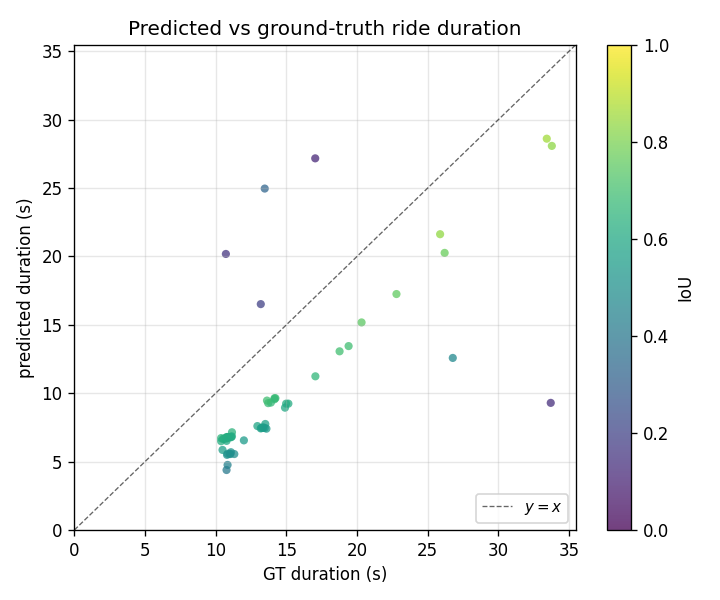
\includegraphics[width=0.6\linewidth]{seg_pred_vs_gt_duration.png}
\caption{Predicted ride duration against hand-edited GT duration
  on every clean match.  Points sit systematically below the
  $y\!=\!x$ diagonal: the GT editor pads each labelled interval
  by~$1$\,s on each side for robustness
  (\S\ref{app:dataset-method}), so the detector's tighter
  intervals lose a constant $\sim 2$\,s of overlap to the pad.
  Correcting for the pad lifts the empirical IoU-F1@0.5 of
  Table~\ref{tab:eval-seg} from $0.83$ towards $0.95$ on the test
  split; the dashed line is the pad-corrected diagonal.}
\label{fig:eval-iou-pad}
\end{figure}

Per-experiment counts, the failure-mode bar chart, and the IoU
distribution are in Appendix~\ref{app:eval-extra-seg}.

\subsection{Per-ride prediction}
\label{sec:eval-pred}

\begin{table}[H]
\centering
\small
\begin{tabular}{llrrrrrrr}
\toprule
Algorithm & Split & $n$ & Median (m) & MAE (m) & $\le 1.5$\,m & $\le 3$\,m & Coverage & Median CI (m) \\
\midrule
Trapezoid & Train & $382$ & $0.27$ & $0.89$ & $88.0\%$ & $93.2\%$ & $87.2\%$ & $1.18$ \\
Trapezoid & Test  & $108$ & $0.29$ & $3.60$ & $90.7\%$ & $91.7\%$ & $93.5\%$ & $1.16$ \\
ZUPT      & Train & $382$ & $0.34$ & $2.32$ & $81.4\%$ & $88.0\%$ & $91.4\%$ & $1.57$ \\
ZUPT      & Test  & $108$ & $0.19$ & $6.45$ & $87.0\%$ & $91.7\%$ & $94.4\%$ & $1.24$ \\
\bottomrule
\end{tabular}
\caption{Per-ride prediction on clean-matched intervals, no
  quality filter.  Median error sits below half a floor on both
  algorithms and both splits; the MAE/RMSE tail comes from a
  small set of damped recordings the quality filter of
  Table~\ref{tab:eval-pipeline} rejects.  Realised coverage at
  the $90\,\%$ nominal holds on the held-out building for both
  algorithms.}
\label{tab:eval-pred}
\end{table}

\begin{figure}[H]
\centering
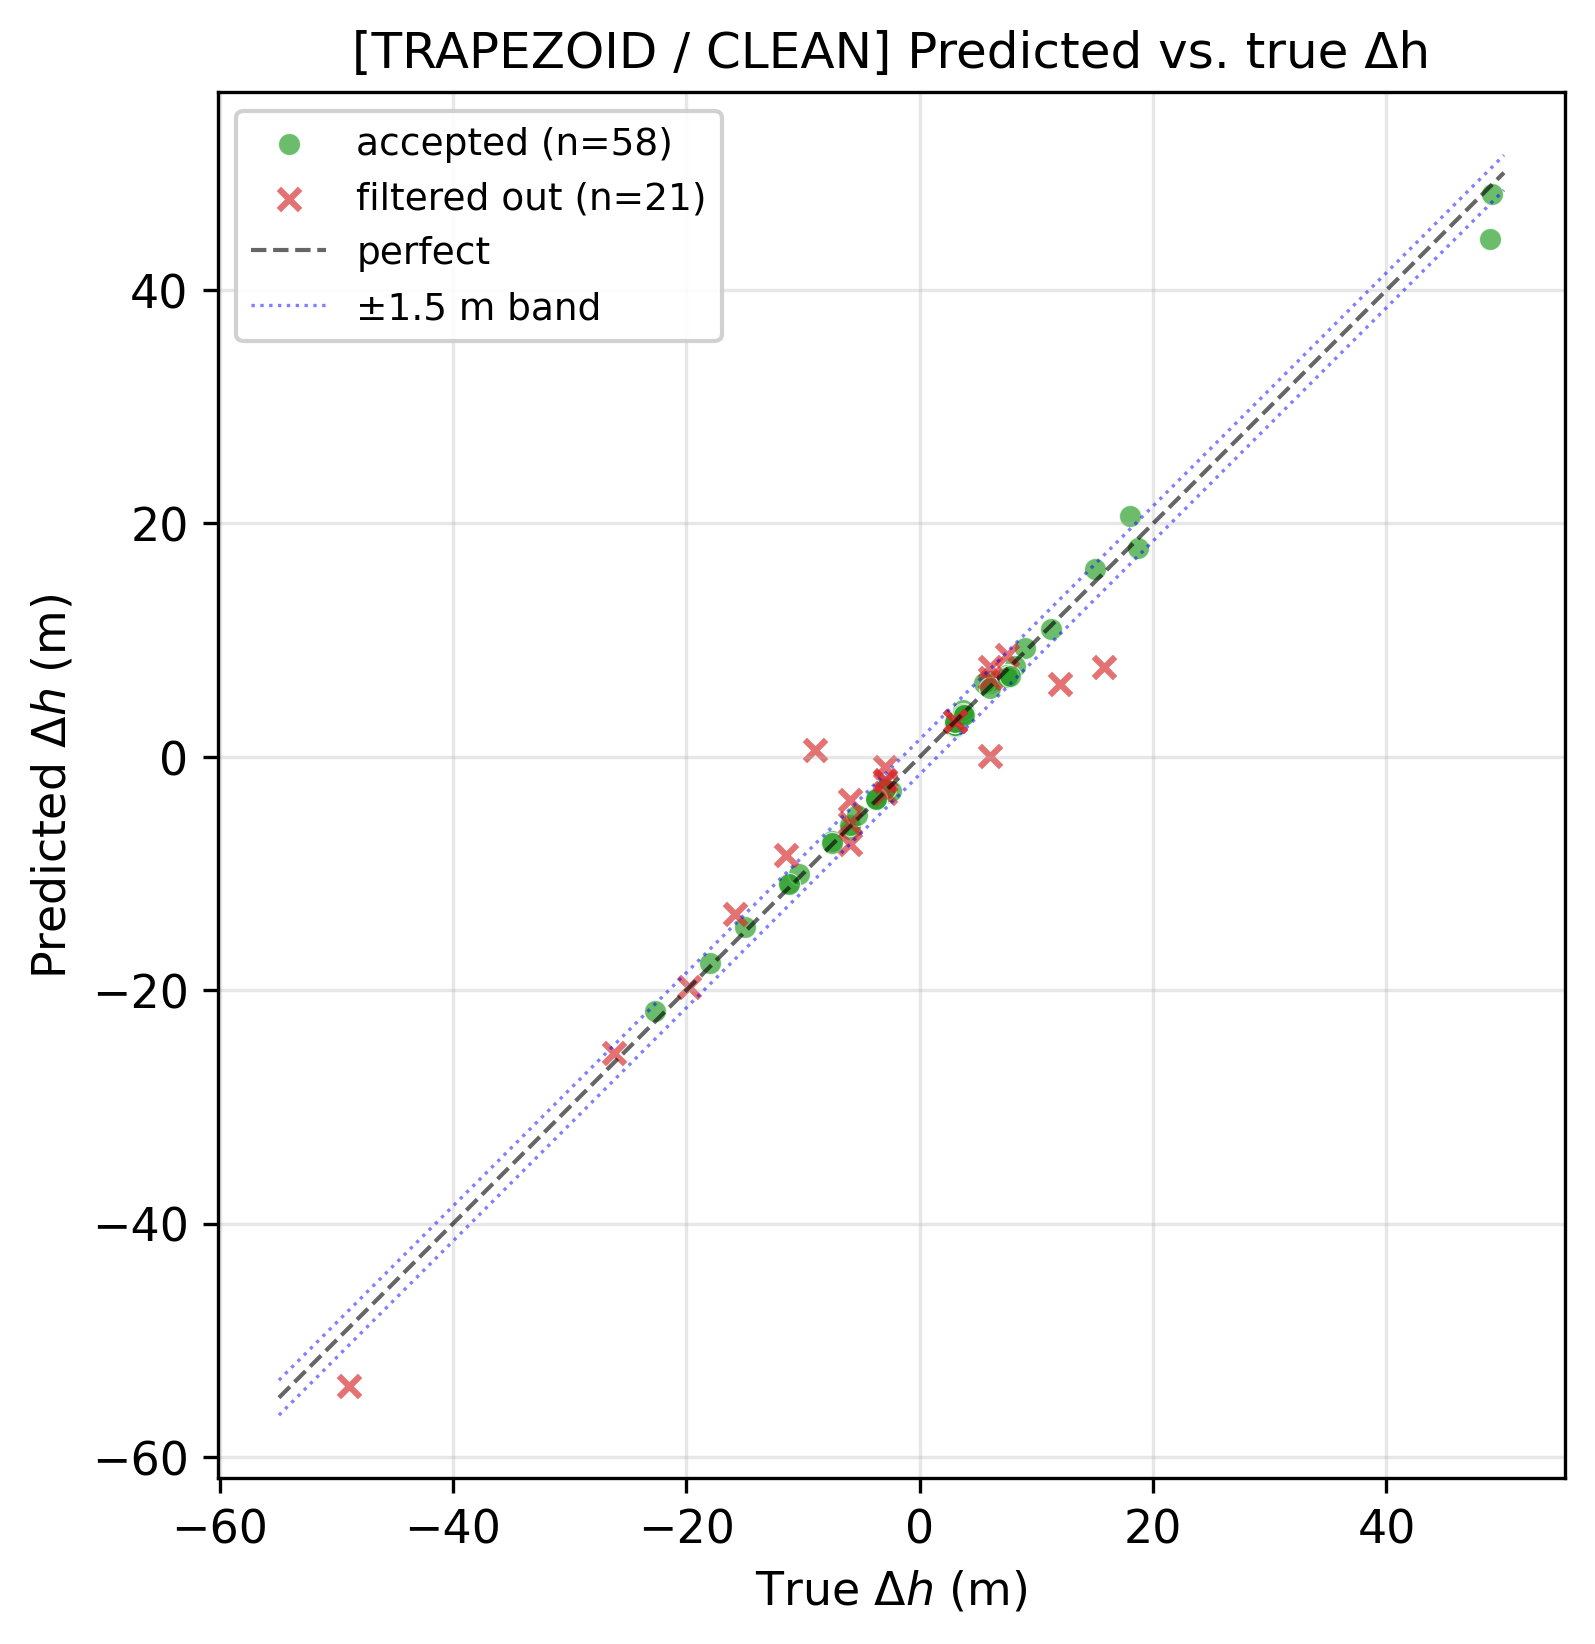
\includegraphics[width=0.7\linewidth]{pred_scatter_trapezoid.png}
\caption{Predicted versus true~$\Delta h$ for the trapezoid fit on
  every clean ride, pooled across train and test.  Points hug the
  $y\!=\!x$ diagonal across more than $40$\,m of $\Delta h$; the
  conformal $90\,\%$ interval is the grey band around each point.
  Per-algorithm scatter and ZUPT comparison sit in
  Appendix~\ref{app:eval-extra-pred}.}
\label{fig:eval-pred-scatter-body}
\end{figure}

Reliability, coverage by ride duration, and per-experiment error
breakdowns are in Appendix~\ref{app:eval-extra-pred}.

\subsection{End-to-end pipeline}
\label{sec:eval-pipeline}

\begin{table}[H]
\centering
\small
\begin{tabular}{llrrrrrr}
\toprule
Algorithm & Split & $n$ & Accept rate & Median (m) & MAE (m) & $\le 1.5$\,m & Coverage \\
\midrule
Trapezoid & Train & $251$ & $66\%$ & $0.18$ & $0.38$ & $93.2\%$ & $92.4\%$ \\
Trapezoid & Test  & $\phantom{0}89$ & $82\%$ & $0.22$ & $0.44$ & $96.6\%$ & $97.8\%$ \\
ZUPT      & Train & $332$ & $87\%$ & $0.26$ & $0.73$ & $90.4\%$ & $94.0\%$ \\
ZUPT      & Test  & $100$ & $93\%$ & $0.14$ & $0.51$ & $93.0\%$ & $98.0\%$ \\
\bottomrule
\end{tabular}
\caption{Deployed pipeline on accepted predictions only
  (segmenter $\to$ predictor $\to$ quality filter).  The filter
  halves mean error on the test split, raises the one-floor-target
  rate past $93\,\%$, and lifts realised coverage past the
  nominal~$90\,\%$ on every row.  Every false positive on the
  held-out test ($9$ of $108$ segmenter predictions) is rejected
  by the filter; the consumer sees zero phantom rides on
  \texttt{Beit Yitzchaki~B}.}
\label{tab:eval-pipeline}
\end{table}

The accepted-only error CDF and FP diagnostics are in
Appendix~\ref{app:eval-extra-pipeline}.

\section{Discussion}
\label{sec:discussion}

% Headline payoff: the family generalises because its source is physics.
The trapezoid family generalises out of distribution.  On the held-out
building \texttt{Beit Yitzchaki~B} the pipeline reaches segmentation
$F1^{\ast}\!=\!0.88$, a per-ride median trapezoid error of $0.22\,$m,
and zero false positives after the quality filter
(Tables~\ref{tab:eval-seg},~\ref{tab:eval-pipeline}).  Every test-split
score matches or exceeds its train counterpart, and correcting for the
$\pm 1\,$s ground-truth pad raises the raw IoU-F1@0.5 from $0.83$ to
roughly $0.95$ (Figure~\ref{fig:eval-iou-pad}).  Realised coverage
reaches $97.8\,\%$ at a nominal $90\,\%$, and the quality filter halves
the accepted-ride mean error on the test split
(Tables~\ref{tab:eval-pred},~\ref{tab:eval-pipeline}).  The reason is
physical: $j_{\max}$, $a_{\max}$, and $v_{\max}$ come from elevator
design standards, so a family built on those limits applies to any
compliant cabin.

% Limitations: three structural bounds on the result.
Three limits bound the scope of this result.  First, the held-out
evaluation rests on one building --- \texttt{Beit Yitzchaki~B}, a
residential block --- and held-out office and hotel splits remain
future work.  Second, the pipeline returns signed displacement
$\Delta h$, not a floor index; mapping a sequence of $\Delta h$ to
specific floors needs a downstream building-height model the user
supplies.  Third, the family assumes ISO~$18738$-compliant kinematics;
hydraulic lifts, older geared machines, and freight cabins violate the
$(j_{\max},a_{\max},v_{\max})$ bounds of~\eqref{eq:elevator-bounds},
and the quality filter rejects those rides at the
gates~(\S\ref{sec:algo-quality}).

% Calibration slack and the recall cost on the other side.
Realised coverage runs $92$--$98\,\%$ on every row of
Table~\ref{tab:eval-pipeline}, above the nominal $90\,\%$, so the
conformal multipliers ($k\!=\!5.04$ for trapezoid, $k\!=\!2.34$ for
ZUPT) are conservative.  They will tighten on a larger calibration
set: we fit the trapezoid $k$ on $251$ accepted train rides and the
ZUPT $k$ on $332$, and split-conformal intervals shrink
as~$1/\sqrt{n_{\rm cal}}$ (\S\ref{sec:algo-ci}).  Tighter coverage
trades against recall: the same filter rejects $18\,\%$ of clean
trapezoid rides and $7\,\%$ of clean ZUPT rides on the test split
(Table~\ref{tab:eval-pipeline} accept rates $82\,\%$ and $93\,\%$).
Each gate threshold in Tables~\ref{tab:seg-thresholds},
\ref{tab:quality-checks-zupt}, and~\ref{tab:quality-checks} is a
single scalar, so a deployment can pick its own coverage--recall
operating point.

\section{Conclusion}
\label{sec:conclusion}

We turned a smartphone into a per-ride elevator-displacement sensor
with a calibrated $90\,\%$ confidence interval, accelerometer-only, on
a held-out residential building.  The mechanical limits of the cabin
force the gravity-removed acceleration into a small parametric family,
and segmentation and prediction are two fits against that family.
Median trapezoid error on the blind test sits at $0.22\,$m, $96.6\,\%$
of accepted rides land within one floor, and the quality filter passes
zero phantom rides through to the consumer
(Table~\ref{tab:eval-pipeline}).  We release the pipeline, the
labelled multi-building dataset, and the evaluation harness ---
\todo{repository URL}.

\bibliographystyle{ACM-Reference-Format}
\bibliography{references}

\appendix

\section{Theoretical Elevator Pulse Analysis}
\label{app:derivations}

This appendix derives the constants of~\S\ref{sec:bg-time-constants}
from the bounds in~\eqref{eq:elevator-bounds}.
\S\ref{app:bangbang} shows the optimal jerk is bang-bang;
\S\ref{app:time-params} integrates the resulting seven-segment
profile to obtain $T_j$, $T_a$, $T_v$, $T_{\text{ride}}$, and the
centroid-spacing identity used in~\S\ref{sec:bg-family}.

\subsection{The optimal elevator pulse}
\label{app:bangbang}

The time-optimal control problem~\eqref{eq:elevator-opt} forces the
optimal jerk to take only three values,
$j^{*}(t)\!\in\!\{-j_{\max},0,+j_{\max}\}$~\eqref{eq:bang-bang}.  We
sketch the three moves Pontryagin's maximum principle turns on; the
full machinery is standard for time-optimal control of a chain of
integrators with bounded input~\cite{athans1966,kirk2004}.

\paragraph{Hamiltonian.}
Stack the state $x=(h,v,a)^{\top}$ with dynamics
$\dot x=(v,\,a,\,j)^{\top}$, control~$j$, free terminal time~$T$,
and unit running cost.  Adjoining co-states
$\lambda=(\lambda_h,\lambda_v,\lambda_a)^{\top}$ gives
\[
  \mathcal H(x,\lambda,j)
  \;=\; 1 + \lambda_h v + \lambda_v a + \lambda_a j,
\]
which is linear in~$j$.

\paragraph{Switching law.}
Linearity in~$j$ pins the PMP-minimising control to the boundary
$|j|=j_{\max}$ whenever $\lambda_a\!\neq\!0$:
\[
  j^{*}(t)\;=\;-j_{\max}\,\operatorname{sign}\lambda_a(t).
\]
The co-state equations $\dot\lambda=-\partial\mathcal H/\partial x$
yield
$\lambda_a(t)=\tfrac12\lambda_h t^{2}-\lambda_v(0)\,t+\lambda_a(0)$,
a quadratic that crosses zero at most twice; the unconstrained
$j^{*}$ therefore switches sign at most twice.

\paragraph{Constrained arcs.}
When $|a|\!=\!a_{\max}$ activates, the cabin rides the boundary and
the controller must hold $\dot a\!=\!j\!=\!0$; the velocity
constraint $|v|\!=\!v_{\max}$ similarly forces $a\!=\!0$ and hence
$j\!=\!0$.  Stitching the unconstrained $\pm j_{\max}$ arcs with
these constrained zero-jerk arcs yields~\eqref{eq:bang-bang} and
the three regimes selected by the floor-to-floor height~$H$
(Figure~\ref{fig:scurve-durations}).

\subsection{Time parameters formula development}
\label{app:time-params}

\begin{wrapfigure}{r}{0.34\linewidth}
  \vspace{-0.8em}
  \centering
  \resizebox{\linewidth}{!}{%
  \begin{tikzpicture}[>=Stealth, font=\footnotesize]
    \pgfmathsetmacro{\Tj}{1.0}
    \pgfmathsetmacro{\Ta}{1.4}
    \pgfmathsetmacro{\amax}{1.5}
    \pgfmathsetmacro{\tA}{\Tj}
    \pgfmathsetmacro{\tB}{\Tj+\Ta}
    \pgfmathsetmacro{\tC}{2*\Tj+\Ta}
    \fill[red!22]    (0,0)   -- (\tA,0) -- (\tA,\amax) -- cycle;
    \fill[orange!22] (\tA,0) -- (\tB,0) -- (\tB,\amax) -- (\tA,\amax) -- cycle;
    \fill[red!22]    (\tB,0) -- (\tC,0) -- (\tB,\amax) -- cycle;
    \draw[->] (-0.15,0) -- ({\tC+0.45},0) node[right] {$t$};
    \draw[->] (0,-0.22) -- (0,{\amax+0.4}) node[above] {$a(t)$};
    \draw[dashed,gray!55] (0,\amax) -- (\tC,\amax);
    \node[left,font=\scriptsize] at (0,\amax) {$a_{\max}$};
    \draw[very thick, blue!70!black]
      (0,0) -- (\tA,\amax) -- (\tB,\amax) -- (\tC,0);
    \draw[dotted,gray!55] (\tA,0) -- (\tA,\amax);
    \draw[dotted,gray!55] (\tB,0) -- (\tB,\amax);
    \node[red!75!black,font=\scriptsize]
          at ({0.55*\Tj},{0.32*\amax}) {$\tfrac12 a_{\max}T_j$};
    \node[orange!85!black,font=\scriptsize]
          at ({\tA+0.5*\Ta},{0.50*\amax}) {$a_{\max}T_a$};
    \node[red!75!black,font=\scriptsize]
          at ({\tB+0.45*\Tj},{0.32*\amax}) {$\tfrac12 a_{\max}T_j$};
    \draw[decorate,decoration={brace,amplitude=2.5pt,mirror},semithick,red!75!black]
      (0,-0.07) -- (\tA,-0.07)
      node[midway,below=-1pt,red!75!black,font=\scriptsize] {$T_j$};
    \draw[decorate,decoration={brace,amplitude=2.5pt,mirror},semithick,orange!85!black]
      (\tA,-0.07) -- (\tB,-0.07)
      node[midway,below=-1pt,orange!85!black,font=\scriptsize] {$T_a$};
    \draw[decorate,decoration={brace,amplitude=2.5pt,mirror},semithick,red!75!black]
      (\tB,-0.07) -- (\tC,-0.07)
      node[midway,below=-1pt,red!75!black,font=\scriptsize] {$T_j$};
  \end{tikzpicture}}
  \vspace{-0.4em}
\end{wrapfigure}
We integrate the bang-bang jerk over the take-off lobe
(phases~1--3), recover the three durations, and sum to the total
ride time.  We assume the trapezoidal regime $T_v\!>\!0$; the
medium and short regimes are limits
$H\!\downarrow\!a_{\max}T_j(T_j+T_a)$ of the same formulas.  Each
phase paints one slab of the lobe beside: the two red wedges of
phases~1 and~3, the orange plateau of phase~2.  Their areas are
the velocity gained on that phase, and the colours below match
the equations.

\paragraph{Phase~1 --- jerk ramp ($j=+j_{\max}$).}
With $a(0)\!=\!v(0)\!=\!0$, one integration gives
\[
  a(t) = j_{\max}\,t,
  \qquad
  a(T_j)=a_{\max}\;\Longrightarrow\;
  T_j=\tfrac{a_{\max}}{j_{\max}}\quad\eqref{eq:Tj}.
\]
Integrating twice more,
\[
  \textcolor{red!75!black}{v(T_j)=\tfrac12\,a_{\max}T_j},
  \qquad
  h(T_j)=\tfrac16\,a_{\max}T_j^{2}.
\]
The velocity $v(T_j)$ is the area of the phase-1 red wedge.

\paragraph{Phase~2 --- acceleration plateau ($a=a_{\max}$).}
On $t\in[T_j,T_j+T_a]$ the cabin holds at $a_{\max}$, so the
velocity gains the area of the orange rectangle,
\[
  v(T_j+T_a) \;=\; v(T_j)+\textcolor{orange!85!black}{a_{\max}T_a}
             \;=\; a_{\max}\!\left(\tfrac12 T_j+T_a\right),
\]
and the displacement added is
$\Delta h_{2} = v(T_j)\,T_a+\tfrac12 a_{\max}T_a^{2}$.

\paragraph{Phase~3 --- jerk ramp-down ($j=-j_{\max}$).}
On $t\in[T_j+T_a,2T_j+T_a]$, $a(t)=a_{\max}-j_{\max}(t-T_j-T_a)$ so
$a(2T_j+T_a)\!=\!0$ as required.  Phase~3 contributes a second
$\tfrac12 a_{\max}T_j$ of velocity --- the mirror red wedge --- so
the lobe-end velocity is the sum of three slab areas,
\[
  v(2T_j+T_a)
  \;=\; \textcolor{red!75!black}{\tfrac12 a_{\max}T_j}
       +\textcolor{orange!85!black}{a_{\max}T_a}
       +\textcolor{red!75!black}{\tfrac12 a_{\max}T_j}
  \;=\; a_{\max}(T_j+T_a).
\]
Demanding the cruise enter at the velocity ceiling,
$a_{\max}(T_j+T_a)\!=\!v_{\max}$, gives
$T_a=\tfrac{v_{\max}}{a_{\max}}-T_j$~\eqref{eq:Ta}.  The
displacement added in phase~3 is
\(
  \Delta h_{3} = v(T_j+T_a)\,T_j+\tfrac12 a_{\max}T_j^{2}
                -\tfrac16 j_{\max}T_j^{3}.
\)

\paragraph{Synthesis.}
Summing phases~1--3 with $j_{\max}T_j\!=\!a_{\max}$ and
$a_{\max}(T_j+T_a)\!=\!v_{\max}$ collapses to
\[
  d_{\text{accel}}
  \;=\; h(T_j)+\Delta h_{2}+\Delta h_{3}
  \;=\; \tfrac12\,v_{\max}\,(2T_j+T_a).
\]
By symmetry phases~5--7 contribute the same $d_{\text{accel}}$.
The cruise covers the remainder $H-2d_{\text{accel}}$ at $v_{\max}$,
\[
  \textcolor{teal!70!black}{T_v
    \;=\; \frac{H-v_{\max}(2T_j+T_a)}{v_{\max}}
    \;=\; \frac{H}{v_{\max}}-2T_j-T_a}
  \quad\eqref{eq:Tv},
\]
and $T_{\text{ride}}\!=\!4T_j+2T_a+T_v$ collapses to the additive
form~\eqref{eq:elevator-durations}.

\paragraph{Centroid spacing of the two acceleration lobes.}
The first lobe spans $[0,\,2T_j+T_a]$ with centroid at
$t_{c,1}\!=\!T_j+T_a/2$ (trapezoid symmetry); the second spans
$[2T_j+T_a+T_v,\,4T_j+2T_a+T_v]$ with centroid at
$t_{c,2}\!=\!3T_j+3T_a/2+T_v$.  Subtracting and using~\eqref{eq:Tv},
\[
  \Delta t_{c}
  \;=\; t_{c,2}-t_{c,1}
  \;=\; 2T_j + T_a + T_v
  \;=\; \frac{H}{v_{\max}}.
\]
The temporal gap between the two acceleration lobes
equals~$H/v_{\max}$ and is independent of $j_{\max}$
and~$a_{\max}$ --- the amplitude-free centroid identity used in
the basis-function mapping of~\S\ref{sec:bg-family}.

\subsection{Template-grid bounds from literature machine parameters}
\label{app:template-grid-bounds}

The segmentation appendix's template grid
(Appendix~\ref{app:seg-matched-filter}) ranges over a discrete set
of~$(W,f)$ cells.  The grid limits are not free parameters --- they
fall out of the kinematic identities
\eqref{eq:W-from-kinematics}--\eqref{eq:f-from-kinematics} once the
literature ranges for the three machine parameters are plugged in.

\paragraph{Literature ranges.}
Section~\ref{sec:bg-bounds} cites the following bounds for commercial
passenger elevators:
\begin{equation}
  j_{\max}\in[1.0,\,1.6]\text{\,m/s$^3$~\cite{iso18738}},\qquad
  a_{\max}\in[0.8,\,1.5]\text{\,m/s$^2$},\qquad
  v_{\max}\in[1.0,\,2.5]\text{\,m/s~\cite{cibseguidd2020}}.
  \label{eq:lit-bounds}
\end{equation}

\paragraph{Time constants.}
Equation~\eqref{eq:Tj} gives the jerk ramp
$T_j=a_{\max}/j_{\max}$, whose range under~\eqref{eq:lit-bounds} is
\[
  T_j \;\in\;
  \left[\tfrac{a_{\min}}{j_{\max}},\,\tfrac{a_{\max}}{j_{\min}}\right]
  \;=\;
  \bigl[0.50,\,1.50\bigr]\text{\,s.}
\]
Equation~\eqref{eq:Ta} gives the acceleration plateau
$T_a=\max(0,\,v_{\max}/a_{\max}-T_j)$; its lower bound is $0$ (any
configuration with $v_{\max}/a_{\max}\le T_j$ saturates the
$a_{\max}$ rail but never reaches $v_{\max}$), and its upper bound
is attained at $v_{\max}\!=\!2.5$, $a_{\max}\!=\!0.8$,
$j_{\max}\!=\!1.6$, yielding
\[
  T_a \;\in\;\bigl[0,\;2.63\bigr]\text{\,s.}
\]

\paragraph{Half-width $W$ and flat fraction $f$.}
Substituting the eight corner combinations of~\eqref{eq:lit-bounds}
into~\eqref{eq:W-from-kinematics}--\eqref{eq:f-from-kinematics}
yields
\[
  W \;\in\;\bigl[0.88,\,1.96\bigr]\text{\,s,}\qquad
  f \;\in\;\bigl[0,\,0.72\bigr].
\]
The lower end of~$f$ is the triangle limit ($T_a\!=\!0$, short hops
that never reach the $a_{\max}$ plateau); the upper end is the
near-rectangular plateau of the longest cruises.

\paragraph{The deployed grid.}
The detector pads these analytical bounds to absorb sensor noise,
controllers that depart from the textbook bang-bang law, and a
margin for the short-ride triangle row.  The deployed grid is
30~log-spaced~$W$ in $[0.4,\,3.0]$\,s and 15~linear~$f$ in
$[0.05,\,0.80]$, plus an explicit $f\!=\!0$ triangle row for short
rides that never reach the $a_{\max}$ plateau.  The same grid is
reused by every stage that fits the trapezoid family
(Appendices~\ref{app:seg-matched-filter} and~\ref{app:prediction}).

\section{Dataset collection and ground-truth pipeline}
\label{app:dataset}

The dataset is 195 labelled elevator rides drawn from eight recording
sessions across seven elevators in six buildings, all collected in
March--April 2026. This appendix walks the construction pipeline
end-to-end: how each session was recorded and how every ride got its
label and floor-to-floor~$\Delta h$~(\S\ref{app:dataset-method}), the
human-in-the-loop edit pass that corrects detector
mistakes~(\S\ref{app:dataset-editing}), and the per-session statistics
of the campaign~(\S\ref{app:dataset-buildings}).

\subsection{Method}
\label{app:dataset-method}

\paragraph{Recording setup.}
Each session ran four phones simultaneously, carried together in one bag
or hand so every device saw the same motion, vibration, and acoustics.
Two experimenters carried two phones each, and the fleet always included
at least one barometer-equipped device whose pressure trace became the
ground truth for the three accelerometer-only phones. Two of the eight
sessions --- Haari~3 and Bar-Ilan~2 --- relied on a single
experimenter holding one barometer-equipped phone.
Table~\ref{tab:app-sensors} lists the channels each phone logged at its
native rate; the loader resamples every channel to 50~Hz before
downstream stages see it.

\paragraph{Barometric pressure to altitude.}
The recording phone's pressure channel converts to a metric altitude
trace through the International Standard Atmosphere troposphere
inversion, $h = (T_0/L)\,[\,1 - (P/P_0)^{1/5.255}\,]$, with the
surface temperature $T_0$ read from the session log.
Figure~\ref{fig:app-barometer-extraction} plots both sides on a
Millennium-Hotel session. Pressure climbs by ${\sim}6$\,hPa as the
experimenter descends from floor~12 to the ground lobby, and the
inverted altitude resolves the matching ${\sim}50$\,m descent on the
same time axis. At standard $T_0$ the resolution sits near $10$\,cm
per sample, an order of magnitude below the ${\sim}3$\,m typical
inter-floor pitch, so floor-to-floor steps stand clear of sensor noise.

\begin{figure}[!htbp]
  \centering
  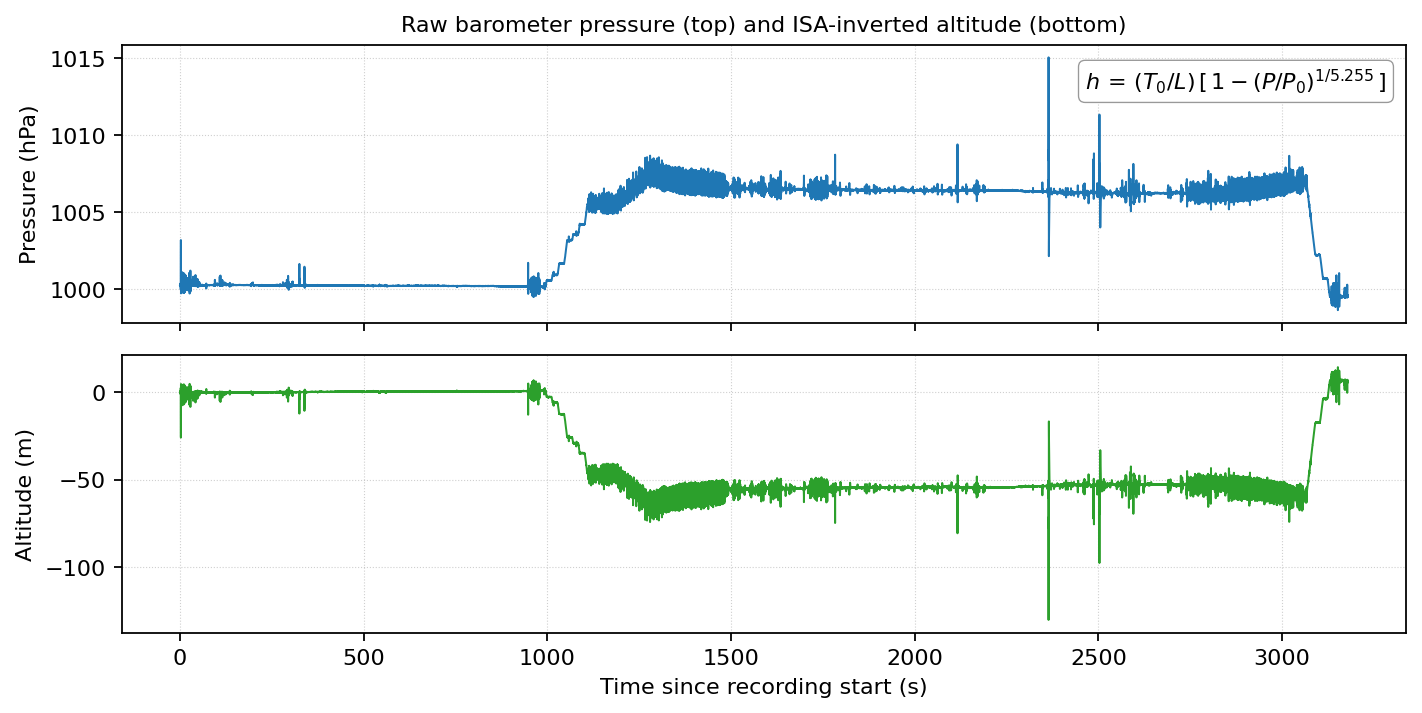
\includegraphics[width=0.68\linewidth]{barometer_extraction.png}
  \caption{Pressure (\textbf{top}) and the ISA-inverted altitude
    (\textbf{bottom}) on a Millennium-Hotel session. The pressure
    rise around $t \approx 1000$\,s is the experimenter taking the
    elevator down from floor~12; the inverted altitude shows the
    matching ${\sim}50$\,m descent.}
  \label{fig:app-barometer-extraction}
\end{figure}

\paragraph{Edge-point ride extraction.}
\texttt{HeightSegmenter} turns the altitude trace into ride intervals
through a deterministic state machine over vertical velocity. The
procedure low-pass filters altitude across an 8\,s rolling window,
differences the result into velocity, smooths velocity with a 3\,s
box kernel, and marks samples above $|v_z| > 0.15$\,m/s as moving.
Same-sign moving runs within 6\,s of each other merge into one
interval. The detector then drops any survivor shorter than 3\,s or
with $|\Delta z| < 2$\,m. The pipeline pads each remaining survivor
by 1\,s on either side and labels it \texttt{up} when the mean
velocity is positive, \texttt{down} otherwise; gaps carry the
\texttt{outside} label, so every sample wears one of the three tags.
Figure~\ref{fig:app-edge-detection} runs the procedure on a 170\,s
window of Millennium-Hotel session~exp2. Four step-shaped descents
in the altitude panel become four negative-velocity dips that breach
the threshold, and the bottom panel emits the matching \texttt{down}
intervals interleaved with \texttt{outside} gaps. Every operation is
deterministic, so repeated runs label a recording identically.

\begin{figure}[!htbp]
  \centering
  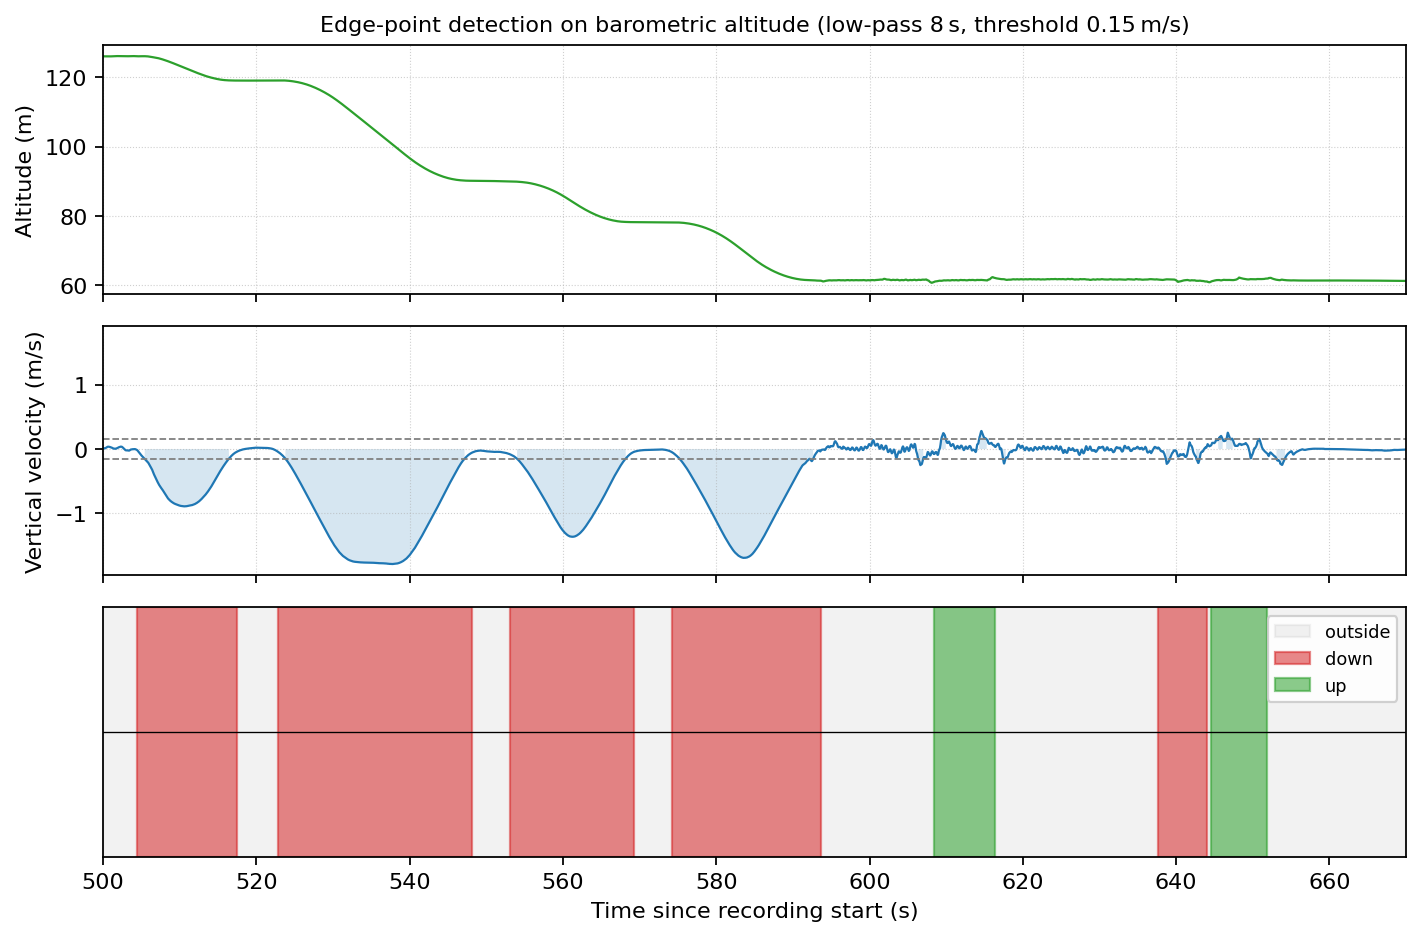
\includegraphics[width=0.68\linewidth]{edge_detection.png}
  \caption{Barometer interval detector on a 170\,s window of
    Millennium-Hotel session~exp2. \textbf{Top:} low-pass altitude.
    \textbf{Middle:} smoothed vertical velocity with the
    $\pm 0.15$\,m/s threshold (dashed) and the ``moving'' regions
    shaded. \textbf{Bottom:} the surviving \texttt{up}/\texttt{down}
    intervals after merging, with \texttt{outside} between them.}
  \label{fig:app-edge-detection}
\end{figure}

\paragraph{Sensor channels.}
An Android logger subscribes to every inertial and environmental
channel the phone exposes and writes one tab-separated row per
sample (Table~\ref{tab:app-sensors}). The pipeline reads accelerometer
(\texttt{ACC}) on every phone, barometer (\texttt{PRS}) on the
equipped phone for ground truth, and gyroscope, magnetometer, and
orientation for the editor's secondary plots and the cross-device
alignment step.

\begin{table}[!htbp]
\centering
\small
\begin{tabular}{lll}
\toprule
\textbf{Tag} & \textbf{Sensor} & \textbf{Columns} \\
\midrule
\texttt{ACC} & Linear accelerometer       & \texttt{x, y, z} \\
\texttt{GYR} & Gyroscope                  & \texttt{x, y, z} \\
\texttt{MAG} & Magnetometer               & \texttt{x, y, z} \\
\texttt{ORI} & Rotation-vector quaternion & \texttt{w, x, y, z} \\
\texttt{PRS} & Barometer                  & \texttt{pressure} \\
\texttt{GPS} & GPS fix                    & \texttt{lat, lon, alt} \\
\bottomrule
\end{tabular}
\caption{Sensor channels emitted by the logger. The pipeline reads
  \texttt{ACC} throughout; \texttt{PRS} supplies ground truth only.}
\label{tab:app-sensors}
\end{table}

\paragraph{Cross-device time synchronisation.}
Android stamps each sample against device boot time, not wall-clock,
so two phones in the same session disagree on event time by their
boot-difference --- often tens of thousands of seconds. The loader
anchors each log on its first-sample timestamp to remove the gross
offset, then sharpens the alignment with a normalised
cross-correlation of the two accelerometer magnitudes across a
$\pm 10$\,s window. After correction the residual lag sits below one
50\,Hz sample, and the pipeline bakes the recovered offset into the
secondary barometer stream before merging.

\paragraph{Gramushka tables and floor snapping.}
Raw barometer altitude drifts with weather and building airflow, so
the pipeline snaps every ride endpoint to a building-specific floor
table.  Figure~\ref{fig:app-gramushka-flow} threads the three steps.
Each building contributes a \emph{gramushka} --- the team's nickname
for the accordion-folded architectural section drawing
(Figure~\ref{fig:app-gramushka}). Transcribing the drawing's labelled
floor lines yields a lookup from floor name to surveyed elevation
(Figure~\ref{fig:app-gramushka-example}). For each detected ride the
pipeline integrates the temperature-aware altitude across the
interval, snaps the endpoint to the nearest floor in the lookup, and
treats the resulting floor-to-floor displacement as the
ground-truth~$\Delta h$ (Figure~\ref{fig:app-gramushka-snap}; the
worked example reads raw $+29.29$\,m and snaps $+1.49$\,m down to
Floor~5 at $+27.80$\,m). The external Millennium elevator has no
drawing; its rides keep the drift-corrected
barometer~$\Delta h$ directly.

\begin{figure}[!htbp]
  \centering
  \begin{subfigure}[c]{0.27\linewidth}
    \centering
    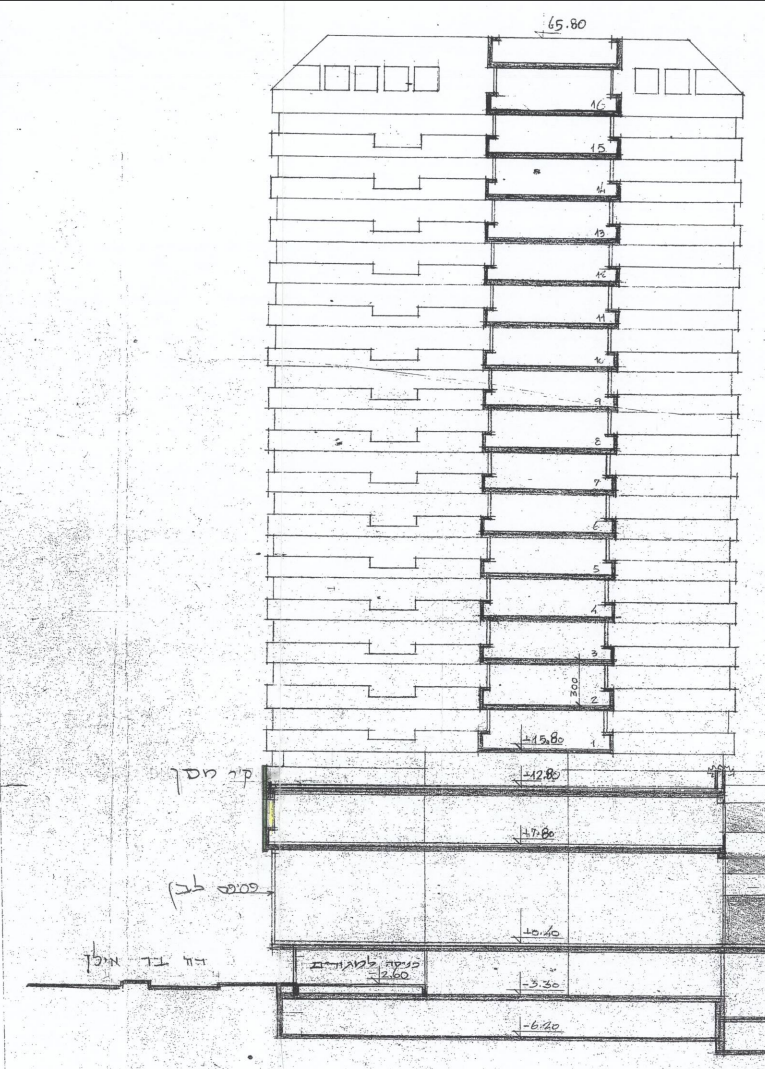
\includegraphics[height=5.0cm,keepaspectratio]{gramushka_drawing.png}
    \caption{Architectural drawing}
    \label{fig:app-gramushka}
  \end{subfigure}%
  \hspace*{0.1em}%
  \raisebox{2.2cm}{\tikz \draw[-Stealth, ultra thick, color=blue!55!black] (0,0) -- (0.7,0);}%
  \hspace*{0.1em}%
  \begin{subfigure}[c]{0.27\linewidth}
    \centering
    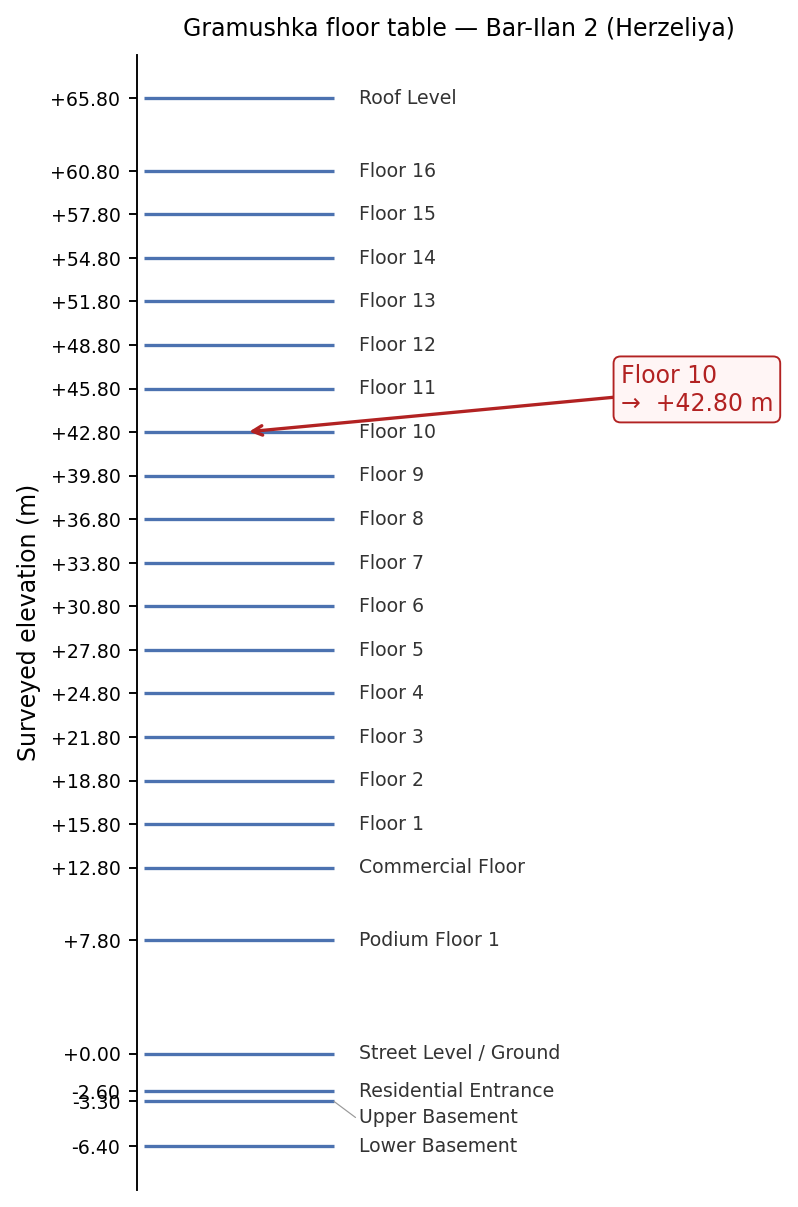
\includegraphics[height=5.0cm,keepaspectratio]{gramushka_example.png}
    \caption{Floor-height lookup}
    \label{fig:app-gramushka-example}
  \end{subfigure}%
  \hspace*{0.1em}%
  \raisebox{2.2cm}{\tikz \draw[-Stealth, ultra thick, color=blue!55!black] (0,0) -- (0.7,0);}%
  \hspace*{0.1em}%
  \begin{subfigure}[c]{0.27\linewidth}
    \centering
    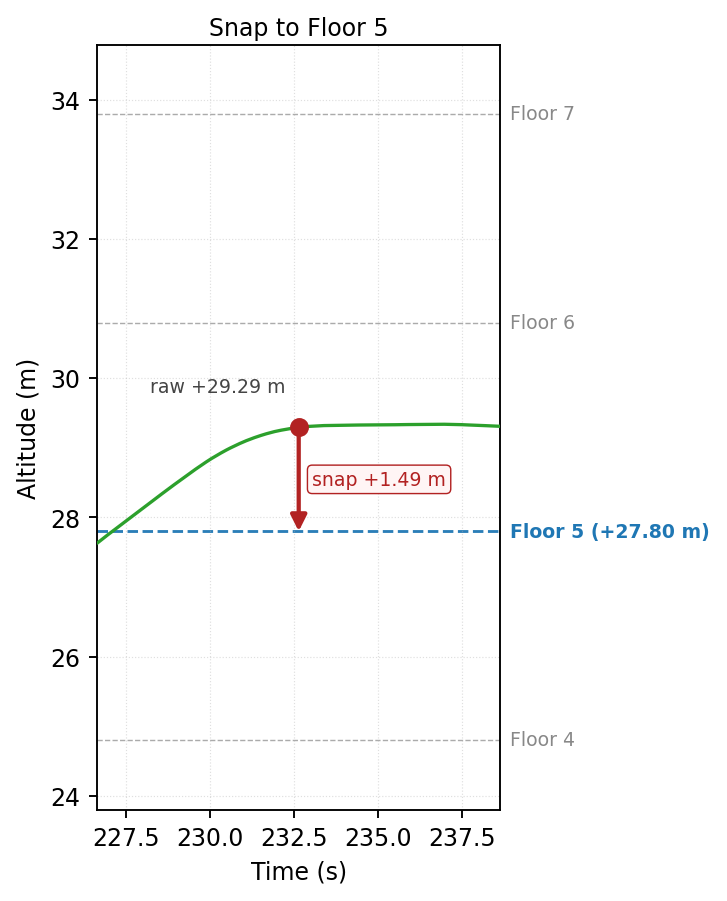
\includegraphics[height=5.0cm,keepaspectratio]{gramushka_snap_panel.png}
    \caption{Snap to nearest floor}
    \label{fig:app-gramushka-snap}
  \end{subfigure}
  \caption{From drawing to floor-height lookup to snapped ride
    endpoint. (\subref{fig:app-gramushka})~The accordion-folded
    architectural section drawing for one campaign building
    (Bar-Ilan~2, Herzeliya). (\subref{fig:app-gramushka-example})~The
    transcribed lookup, mapping each floor name to one surveyed
    elevation (annotated arrow: Floor~10 at $+42.80$\,m).
    (\subref{fig:app-gramushka-snap})~A worked snap from a real
    Bar-Ilan~2 ride: the raw barometer altitude $+29.29$\,m snaps
    $+1.49$\,m down to Floor~5 at $+27.80$\,m.}
  \label{fig:app-gramushka-flow}
\end{figure}

\subsection{Hand editing}
\label{app:dataset-editing}

\paragraph{Why hand editing.}
The barometer detector cannot tell elevator motion from any other
vertical motion of the same magnitude. Stair climbs, driving up or
down a hill, and HVAC pressure ripples each pass the velocity
threshold and slip into the label stream; conversely, an over-tight
merge fuses two close rides into one. Experimenters carry side
information --- which button they pressed, which lobby they entered,
which staircase they took --- that no sensor sees, and the hand-edit
pass injects that knowledge into the labels.

\paragraph{The editor.}
Every recording passes through the ground-truth editor of
Figure~\ref{fig:app-gt-editor} at least once. Stacked panels show
altitude, vertical velocity, and the accelerometer, gyroscope, and
magnetometer magnitudes on a shared time axis; ride intervals overlay
as coloured spans (green~$=$~up, red~$=$~down, grey~$=$~outside). A
side table lists every interval for direct editing, and the
detector's current proposals appear as toggleable hatched bands the
editor can promote, redraw, or reject.

\begin{figure}[!htbp]
  \centering
  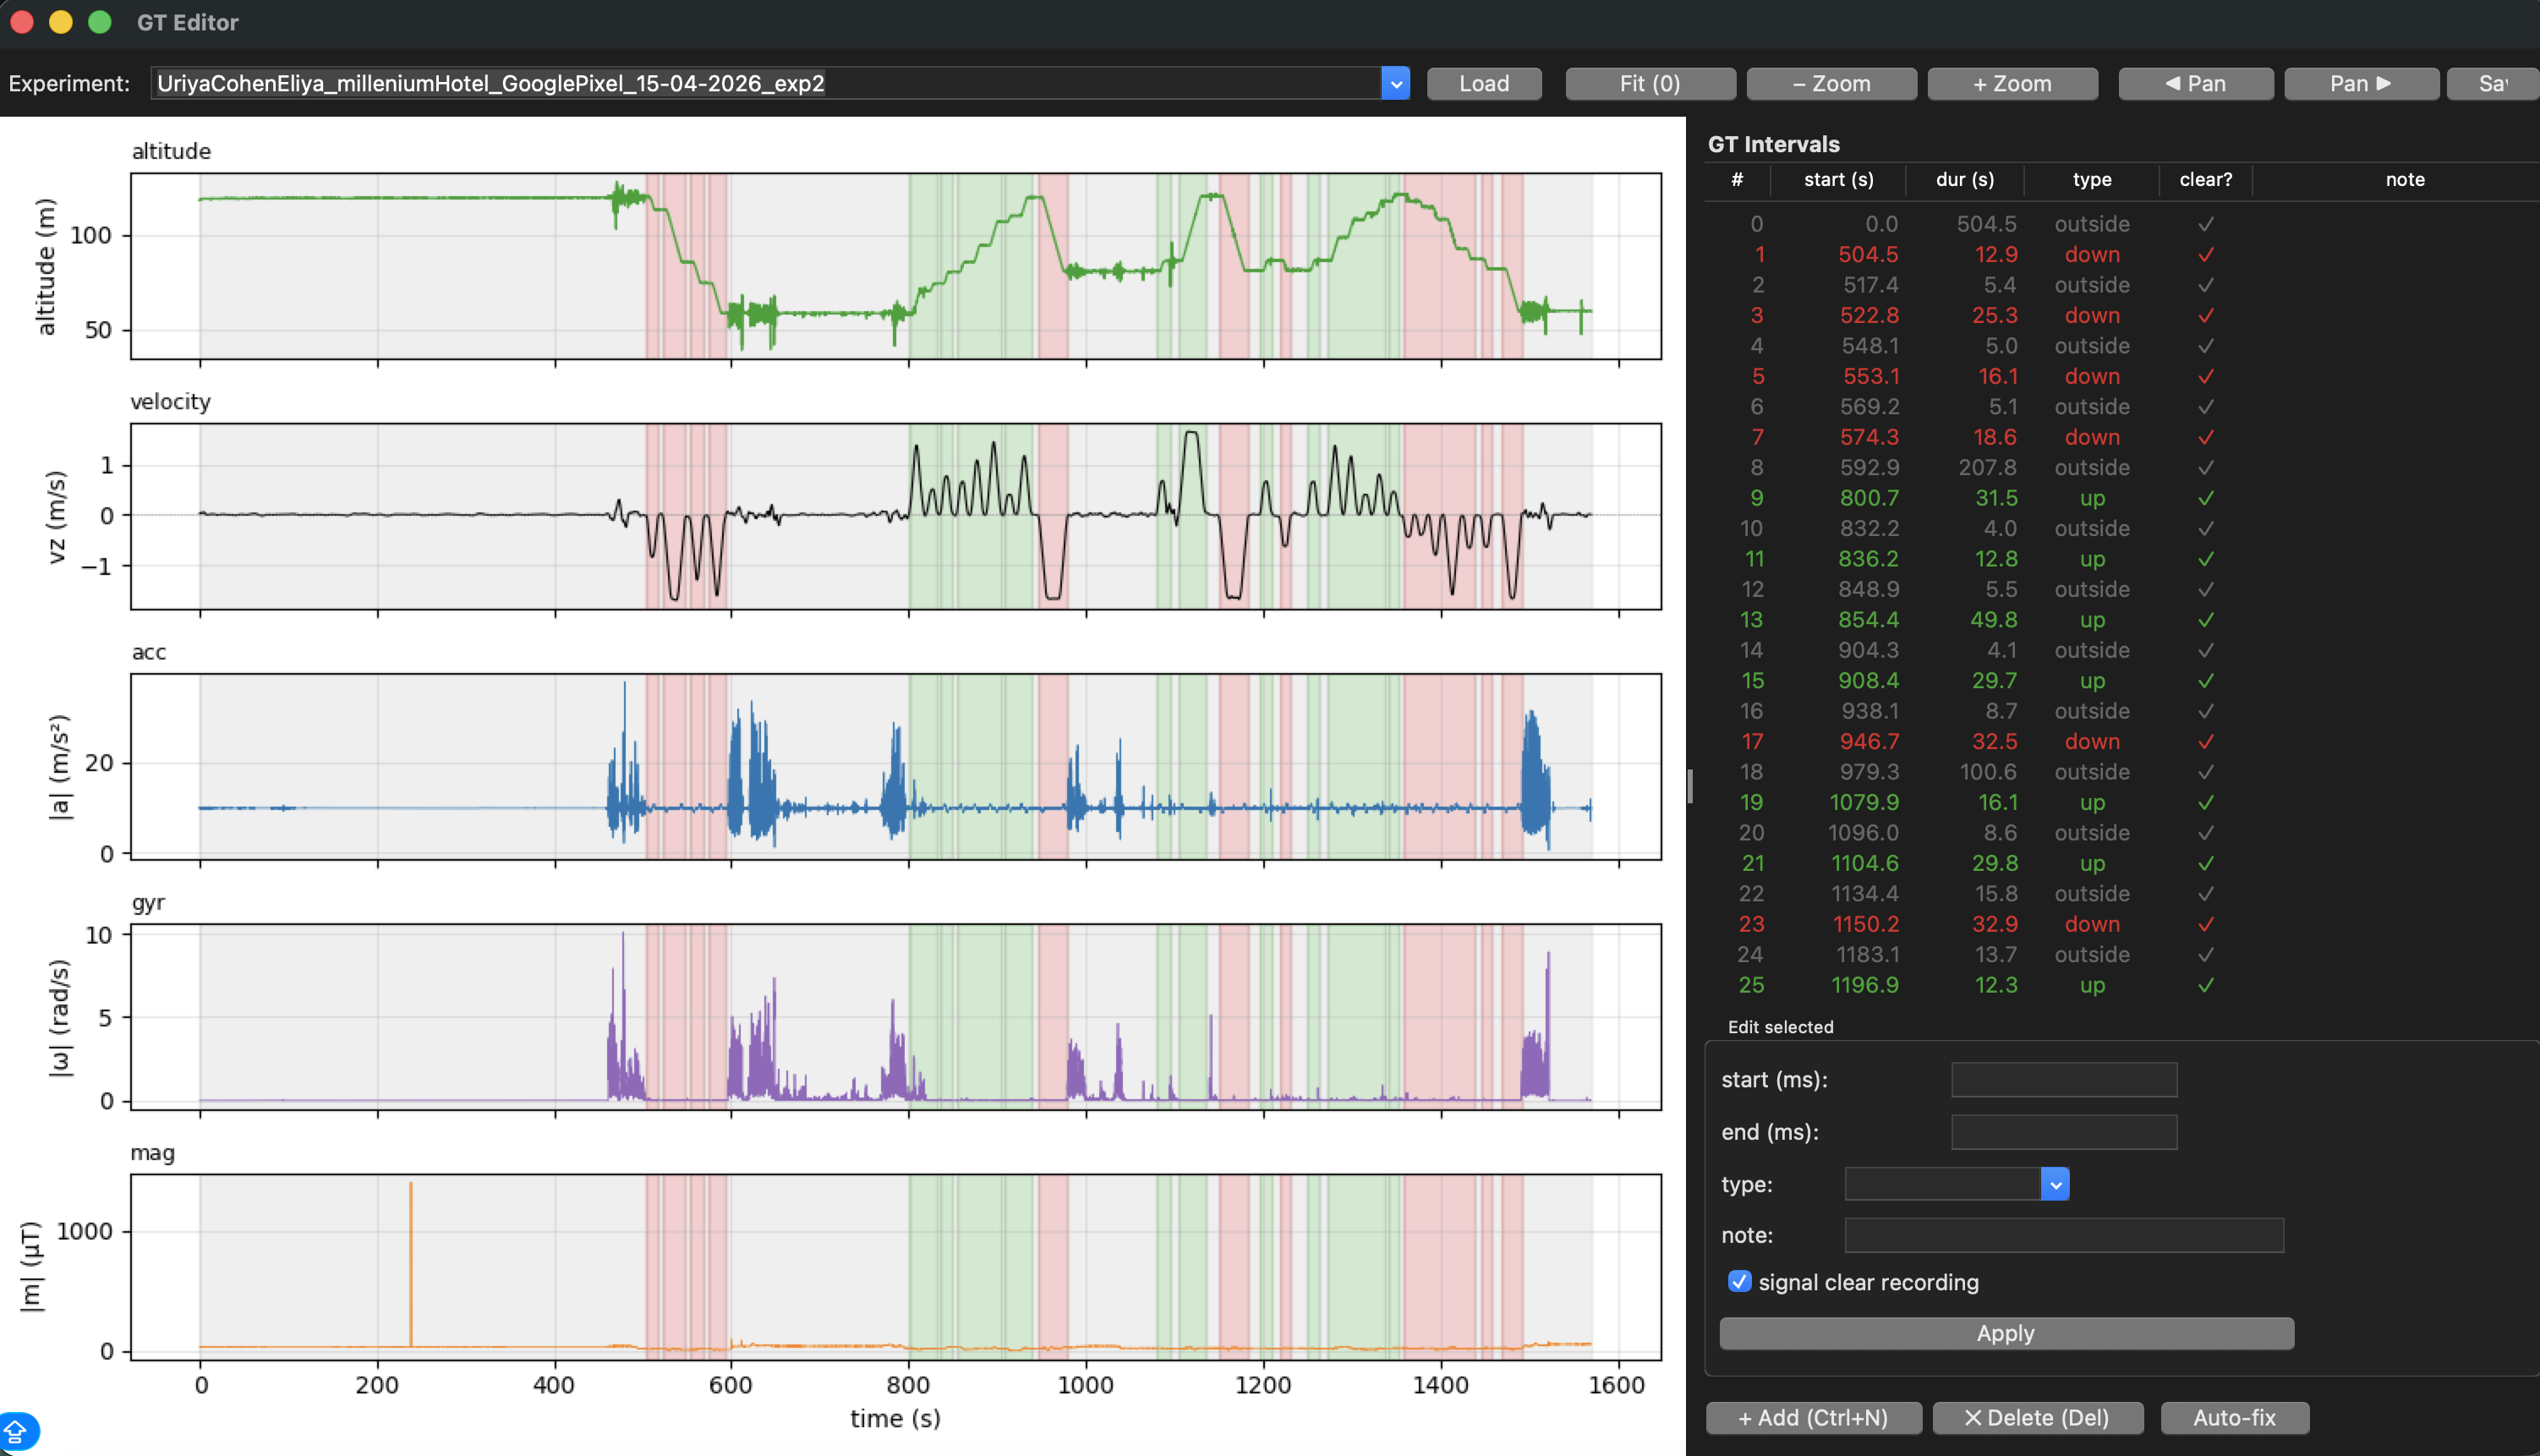
\includegraphics[width=0.70\linewidth]{gt_editor.png}
  \caption{The ground-truth editor. Stacked panels show altitude,
    vertical velocity, and the accelerometer, gyroscope, and
    magnetometer magnitudes on a shared time axis; ground-truth
    intervals are overlaid as coloured spans (green~$=$~up,
    red~$=$~down, grey~$=$~outside). The side table lists every
    interval for direct editing.}
  \label{fig:app-gt-editor}
\end{figure}

\paragraph{What the editor fixes.}
The pass deletes stair-climb and driving-induced intervals the
detector mistook for rides, splits intervals where two consecutive
rides merged across a short pause, and retags any direction the
velocity-sign rule flipped from a low-amplitude pre-ride drift.
Dragging a mis-aligned endpoint on the plot snaps it onto the
altitude step; the editor commits the GT~CSV on save. Every
ground-truth file in the dataset has at least one human-confirmed
pass.

\subsection{Buildings and phones}
\label{app:dataset-buildings}

The campaign covers seven elevators across six buildings in three
Israeli cities --- Ra'anana, Herzeliya, and Ramat Gan --- yielding 195
labelled rides across eight sessions. Six of the eight sessions ran the
standard four-phone fleet (two experimenters $\times$ two phones each):
Google Pixel~10, Samsung Galaxy~A23, Samsung Galaxy~S23, and Xiaomi
Redmi Note~12. The Haari~3 and Bar-Ilan~2 sessions deviated to a
single barometer-equipped phone (Samsung Galaxy Z~Flip6 and Google
Pixel~10 respectively). Ride counts per session range from 10
(Millennium~Hotel exp1) to 44 (Bar-Ilan~2);
Table~\ref{tab:app-sessions} lists every session with its phones,
latitude and longitude where surveyed, building type, and ride count.
\texttt{Beit~Yitzchaki~B} is the held-out blind-test building; the
other seven sessions feed training.

\begin{table}[!htbp]
\centering
\small
\begin{tabular}{lllcc}
\toprule
\textbf{Session} & \textbf{Type} & \textbf{Lat, Long} & \textbf{Phones} & \textbf{Rides} \\
\midrule
Haari~3, Ramat Gan, 2026-04-10            & Residential        & 32.0658, 34.8233      & Z~Flip6                       & 39 \\
Bar-Ilan~2, Herzeliya, 2026-03-24         & Residential        & 32.166394, 34.842190  & Pixel~10                      & 44 \\
Millennium Hotel, exp1, 2026-04-15        & Hotel              & ---                   & Pixel~10, Note~12, A23, S23   & 10 \\
Millennium Hotel, exp2, 2026-04-15        & Hotel              & ---                   & Pixel~10, A23, S23, Note~12   & 31 \\
Millennium Outside, exp3, 2026-04-15      & Hotel (external)   & ---                   & Pixel~10, A23, S23, Note~12   & 12 \\
Acro Building, exp4, 2026-04-15           & Office             & ---                   & Pixel~10, A23, S23, Note~12   & 12 \\
Beit Mansour 1, exp5, 2026-04-15          & Residential        & ---                   & Pixel~10, A23, S23, Note~12   & 18 \\
Beit Yitzchaki~B, exp6, 2026-04-15        & Residential (test) & ---                   & Pixel~10, A23, S23, Note~12   & 29 \\
\bottomrule
\end{tabular}
\caption{The eight recording sessions of the field campaign. Phone
  short names: Pixel~10~$=$~Google Pixel~10,
  A23~$=$~Samsung Galaxy~A23 (SM-A235F),
  S23~$=$~Samsung Galaxy~S23 (SM-S911B),
  Note~12~$=$~Xiaomi Redmi Note~12 (22101320I),
  Z~Flip6~$=$~Samsung Galaxy Z~Flip6. Latitude and longitude are
  recorded for two buildings; the remaining four are kept anonymised
  pending publication.}
\label{tab:app-sessions}
\end{table}

A companion data drop at \todo{<DRIVE-URL>} mirrors the complete
raw sensor logs, gramushka tables, per-session ground-truth CSVs,
and editor screenshots for reproducibility.

\clearpage
\section{Segmentation: matched-filter and pair-filter details}
\label{app:segmentation}
\label{app:thresholds}

This appendix derives the matched-filter solution and the
shared-shape joint score of~\S\ref{sec:algo-seg}, then walks every
calibrated threshold of Table~\ref{tab:seg-thresholds} row by row.
Each subsection takes one row of the table, explains the intuition
behind the test, and --- where the picture is worth more than the
prose --- carries a single illustrative figure.

\begin{table}[H]
\centering
\small
\begin{tabular}{lll}
\toprule
\textbf{Stage / gate} & \textbf{Condition} & \textbf{Threshold} \\
\midrule
Detect: shape floor      & $R^{2}(i)\ge$                  & $0.40$ \\
Detect: amplitude floor  & $|\hat A(i)|\ge$               & $0.20$\,m/s$^{2}$ \\
Detect: peak dedup       & non-max suppression radius     & $1.0$\,s \\
Detect: same-sign gap    & min.\ gap, equal signs         & $5.0$\,s \\
\midrule
Gate 1: temporal gap     & $t(i_2)-t(i_1)\in$             & $[0,30]$\,s \\
Gate 2: joint score      & $\tfrac12(R^{2}_1{+}R^{2}_2)\ge$ & $0.90$ \\
Gate 3: shared amplitude & $A^{\star}\ge$                 & $0.30$\,m/s$^{2}$ \\
Gate 4: grid energy      & $E(i,j)\ge$                    & $0.40$ \\
Gate 5: quiet middle     & $\mathrm{RMS}_{\mathrm{mid}}/A^{\star}\le$ & $0.5$ \\
Gate 6: duration penalty & rank $=S-\lambda\,\Delta t$ & $\lambda=0.01$\,s$^{-1}$ \\
\bottomrule
\end{tabular}
\caption{Calibrated detection and pair-filter thresholds.  The
  kinematics fix the template-grid bounds; a grid search on the
  training experiments chose the acceptance thresholds against a
  composite segmentation metric.  The values shown are the detector's
  deployed defaults.}
\label{tab:seg-thresholds}
\end{table}

\subsection{Matched-filter solution and template grid}
\label{app:seg-matched-filter}

Before the row-by-row walk, we collect the three pieces of machinery
the gates all rely on: the per-window least-squares fit, the
$(W,f)$ template grid that fit ranges over, and the shared-shape
joint score that turns two candidate lobes into one pair fit.

\paragraph{Matched-filter least-squares solution.}
The detector fits each window~$a_{[i]}$ with a single scaled template,
minimising $\|a_{[i]}-A\,\tau_{W,f}\|^{2}$ over~$A$.  The normal
equation $A\,\|\tau_{W,f}\|^{2}=\langle a_{[i]},\tau_{W,f}\rangle$
gives the fitted amplitude and the coefficient of determination
of~\eqref{eq:matched-filter}.  The score~$R^{2}_{W,f}(i)$ is the
window-energy fraction the template explains: $R^{2}\!=\!1$ an exact
fit, $R^{2}\!\le\!0$ no better than the zero signal.

\paragraph{Template grid.}
Appendix~\ref{app:template-grid-bounds} derives the analytical
$(W,f)$ ranges admitted by the commercial machine parameters of
\S\ref{sec:bg-bounds}; the deployed grid pads them to 30~log-spaced
$W$ in $[0.4,\,3.0]$\,s and 15~linear $f$ in $[0.05,\,0.80]$, plus
an $f\!=\!0$ triangle row for short rides that never reach the
$a_{\max}$ plateau.

\paragraph{Shared-shape joint score.}
The pair score~\eqref{eq:joint-fit} fits \emph{one} amplitude to
\emph{both} lobes of a candidate pair.  With~$a_k$ the $k$th lobe
window, $P_k=\|a_k\|^{2}$, $u_k=s_k\langle a_k,\tau_{W,f}\rangle$ the
sign-corrected correlation, and $N=\|\tau_{W,f}\|^{2}$, minimising
$\sum_k\|a_k-s_k A\,\tau_{W,f}\|^{2}$ over the shared~$A$ gives
$A^{\star}=(u_1+u_2)/(2N)$ and the per-lobe~$R^{2}_k$
of~\eqref{eq:joint-fit}.  Unrelated bursts peak at a different cell
for each lobe, so forcing one~$(W,f)$ on both is what makes the score
discriminating.

\subsection{Detection shape and amplitude floors}
\label{app:seg-detect-floors}

The first two rows of Table~\ref{tab:seg-thresholds} reject samples
that cannot be a take-off or
landing lobe at all~\eqref{eq:detect-gate}.  The shape
floor~$r_{\min}\!=\!0.40$ is deliberately permissive: hand-held
jitter and clipped windows pull a real lobe's~$R^{2}$ below a
textbook trapezoid's, so the detector leaves the strict shape test to
the pair stage.  The amplitude floor~$a_{\min}\!=\!0.20$\,m/s$^{2}$
drops lobes buried in sensor and walking noise, and rises per phone
when a device's measured noise runs higher.  Both favour recall ---
a missed lobe is lost for good, while a spurious one still faces the
pairing gates.

\subsection{Peak de-duplication and same-sign gap}
\label{app:seg-detect-dedup}

The next two rows of Table~\ref{tab:seg-thresholds} stop one physical
lobe from entering the pair stage
as several peaks.  A lobe's matched-filter score forms a ridge
several samples wide, so non-maximum suppression over a~$1.0$\,s
radius keeps only its crest, and the same-sign gap collapses any two
\emph{equal}-sign peaks closer than~$5.0$\,s --- a lobe re-detected
at a neighbouring~$W$.  Opposite-sign peaks pass untouched:
separating a take-off from its landing is the pairing stage's task.

\subsection{Gate 1 --- pairing window $[t_{\min},t_{\max}]$}
\label{app:seg-gate1}

Gate~1 bounds how far a take-off and a landing may sit apart before
the pair is scored~\eqref{eq:partner-set} --- a search window, not a
model of ride duration.  The lower bound~$t_{\min}\!=\!0$\,s admits
the shortest single-floor hops, whose lobes almost touch; the upper
bound~$t_{\max}\!=\!30$\,s brackets one uninterrupted ride at the car
speeds and inter-floor heights of vertical-transportation
practice~\cite{strakosch2010,cibseguidd2020}.  A high-rise express
run would need a wider window; the~$30$\,s cap trades that reach
against joining lobes drawn from \emph{different} rides.

\subsection{Gates 2 \& 3 --- joint shape and shared amplitude}
\label{app:seg-gate2}
\label{app:seg-gate3}

Gates~2 and~3 read the same shared-shape fit~\eqref{eq:joint-fit}
from two different angles: a single $(W,f)$ template explaining the
\emph{shapes} of both lobes, and the mean $A^{\star}$ summing their
\emph{amplitudes}.  Both lobes are cut from one cabin profile, so a
real ride must clear both gates; an accidental pairing typically
fails at least one.

Gate~2 demands a joint score of at least~$r_{\mathrm{pair}}\!=\!0.90$,
far above the~$0.40$ detector floor.  Unrelated bursts each fit some
template alone but peak at different cells, so no shared $(W,f)$
scores both above~$0.90$.

Gate~3 requires the shared amplitude~$A^{\star}$ to clear
$a_{\mathrm{pair}}\!=\!0.30\,\mathrm{m/s^{2}}$, above the~$0.20$
detector floor.  Since~$A^{\star}$ is the mean of the two lobe
amplitudes, a pair survives only when \emph{both} lobes are firm: a
strong take-off matched to a weak noise lobe averages below~$0.30$,
even when the joint shape still passes Gate~2.

Together the two floors are cheap --- they cost almost no true rides
while removing the bulk of accidental pairings
(Figure~\ref{fig:thresh-gate2}).

\begin{figure}[H]
\centering
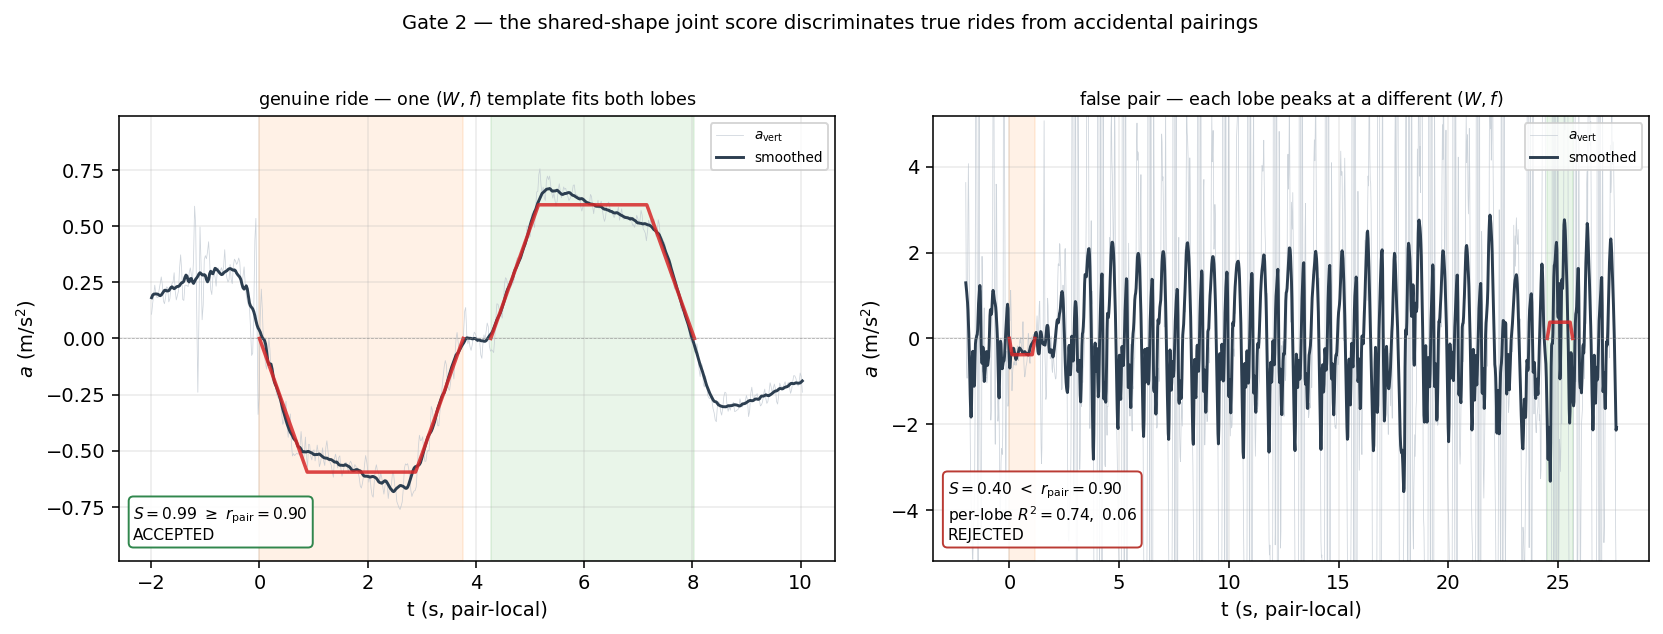
\includegraphics[width=0.6\linewidth]{gate2_joint_score.png}
\caption{Gates~2 and~3 on two real candidate pairs.  \textbf{Left:} a
  genuine ride --- one $(W,f)$ trapezoid (red) overlays both
  opposite-sign lobes; $S\!=\!0.99$ and $A^{\star}$ both clear their
  floors.  \textbf{Right:} an accidental pairing --- one $(W,f)$ fits
  one lobe well ($R^{2}_{1}\!=\!0.74$) but not the other
  ($R^{2}_{2}\!=\!0.06$); $S\!=\!0.40$ falls below the joint-score
  floor and the weak lobe drags $A^{\star}$ below its floor too.}
\label{fig:thresh-gate2}
\end{figure}

\subsection{Gate 4 --- grid energy $e_{\min}$}
\label{app:seg-gate4}

Gate~4 measures \emph{how broadly} the grid supports the match.  A
genuine ride near-fits a whole neighbourhood of~$(W,f)$ templates ---
a wide bright band in the joint-$R^{2}$ heatmap --- while a
coincidental pairing fits one lucky cell and leaves the grid dark.
Grid energy~$E$ averages the clamped joint~$R^{2}$ over every
cell~\eqref{eq:grid-energy}; the floor~$e_{\min}\!=\!0.40$ sits above
a single-cell match and below any broad band, catching false pairs
that clear the best-cell score of Gate~2
(Figure~\ref{fig:thresh-energy}).

\begin{figure}[H]
\centering
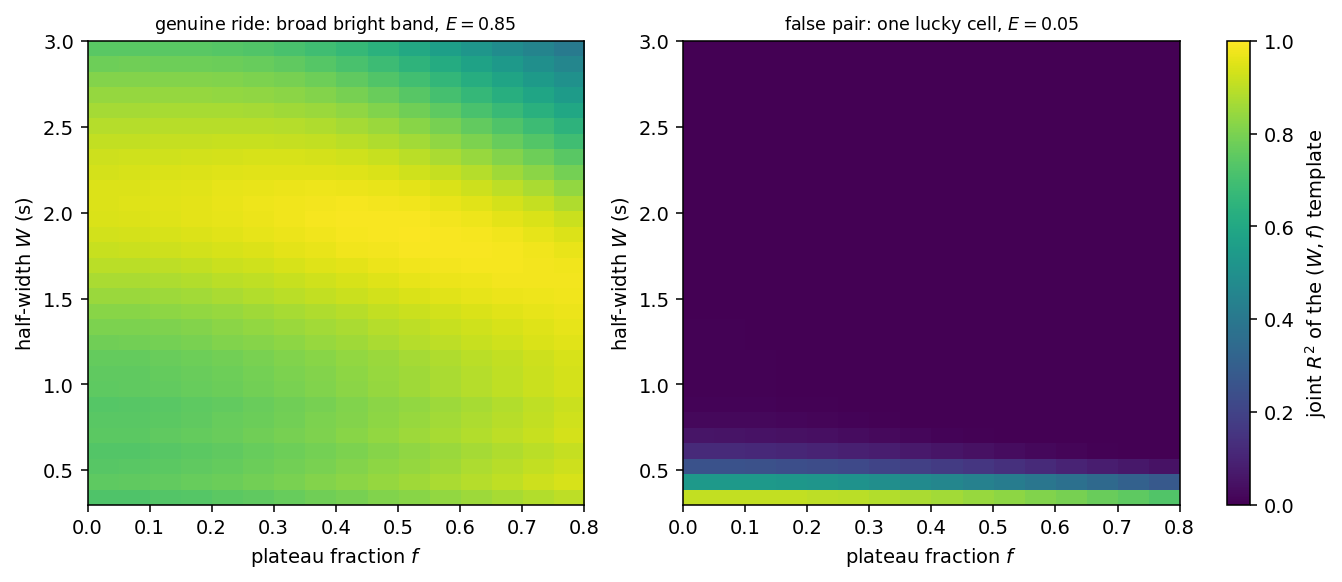
\includegraphics[width=\linewidth]{threshold_grid_energy.png}
\caption{The grid-energy gate~$e_{\min}$.  Each panel is the
  joint-$R^{2}$ heatmap over the~$(W,f)$ template grid for one
  candidate pair.  A genuine ride (left) is a near-fit across a broad
  band of templates, so its grid energy~$E$ sits well above
  the~$0.40$ floor; a coincidental pairing (right) fits one narrow
  sliver and leaves the grid dark, so its energy falls far below the
  floor and Gate~4 rejects it.}
\label{fig:thresh-energy}
\end{figure}

\subsection{Gate 5 --- quiet-middle cruise gate $\rho$}
\label{app:seg-gate5}

Between its two lobes a real ride holds constant velocity, so the
vertical acceleration there is near zero.  Gate~5
takes~$\mathrm{RMS}_{\mathrm{mid}}$, the root-mean-square of the
smoothed acceleration on the inter-lobe
window~$(t_{c_1}\!+\!W,\;t_{c_2}\!-\!W)$, and rejects the pair when
it exceeds~$\rho A^{\star}$ with~$\rho\!=\!0.5$ --- when the cruise
wobble passes half the lobe amplitude.  Equivalently, fit a line
through the cruise samples; the RMS rule rejects pairs whose
regression tilts by more than~$\approx\!15^{\circ}$ from horizontal
(Figure~\ref{fig:thresh-gate5}).  The test catches pairs whose
middle never settles, most often a walking false positive where
continuous motion keeps the inter-lobe stretch as loud as the lobes.

\begin{figure}[H]
\centering
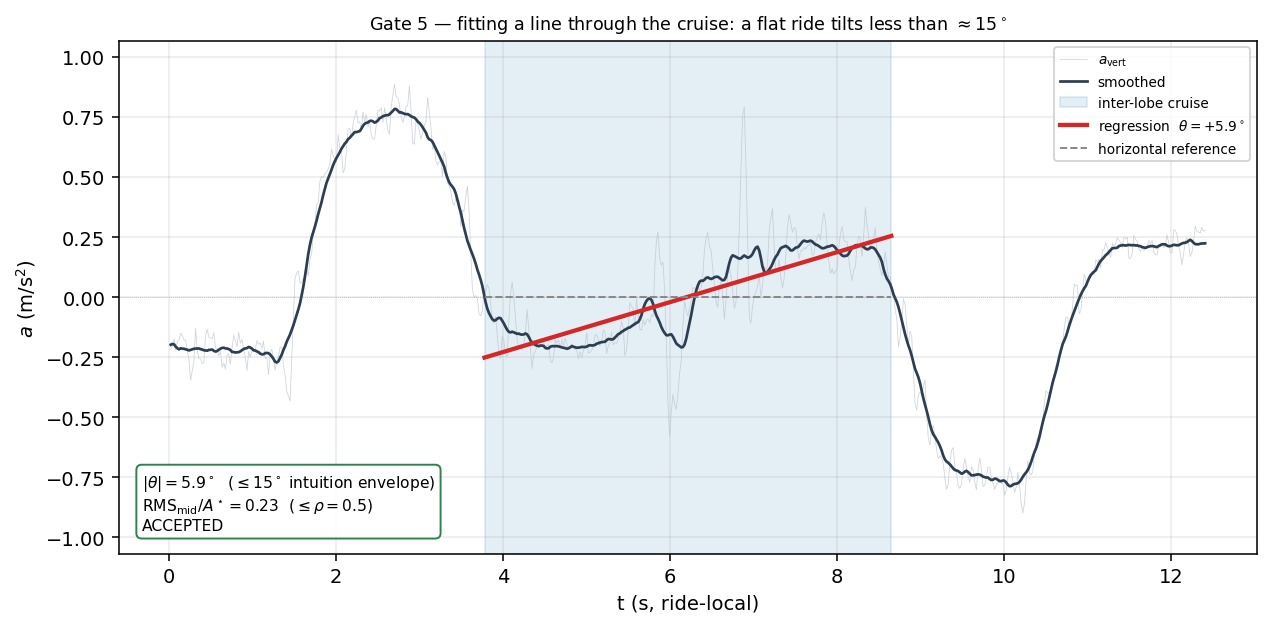
\includegraphics[width=0.85\linewidth]{gate5_cruise_angle.png}
\caption{Gate~5 on the first short ride of a real multi-stop trip
  (the same recording that drives Figure~\ref{fig:thresh-rank}).  A
  least-squares line through the inter-lobe cruise samples (shaded)
  tilts by only $\theta\!=\!5.9^{\circ}$, well inside the
  $\approx\!15^{\circ}$ envelope; equivalently
  $\mathrm{RMS}_{\mathrm{mid}}/A^{\star}\!=\!0.23$ is well under
  $\rho\!=\!0.5$, and the pair is accepted.}
\label{fig:thresh-gate5}
\end{figure}

\subsection{Gate 6 --- duration penalty $\lambda$ and greedy resolution}
\label{app:seg-gate6}

A passenger often rides in stages --- floor~$1$ to~$4$, a stop,
then~$4$ to~$8$ --- recorded as two back-to-back rides and
\emph{four} lobes (Figure~\ref{fig:thresh-rank}).  The take-off of
the first ride and the landing of the last form a \emph{super pair}:
it shares the same cabin shape, so its joint score~$S$ matches either
true ride and Gate~2 cannot tell them apart.  Gate~6 breaks the tie
by ranking every admissible pair by~$S-\lambda\,\Delta t$
with~$\lambda\!=\!0.01$\,s$^{-1}$~\eqref{eq:pair-rank}: the penalty
docks the long span far more than the short ones, so the two short
rides out-rank the super pair.  A greedy resolver commits pairs
highest-first, skipping any that reuse a committed lobe, and the
super pair never commits.

\begin{figure}[H]
\centering
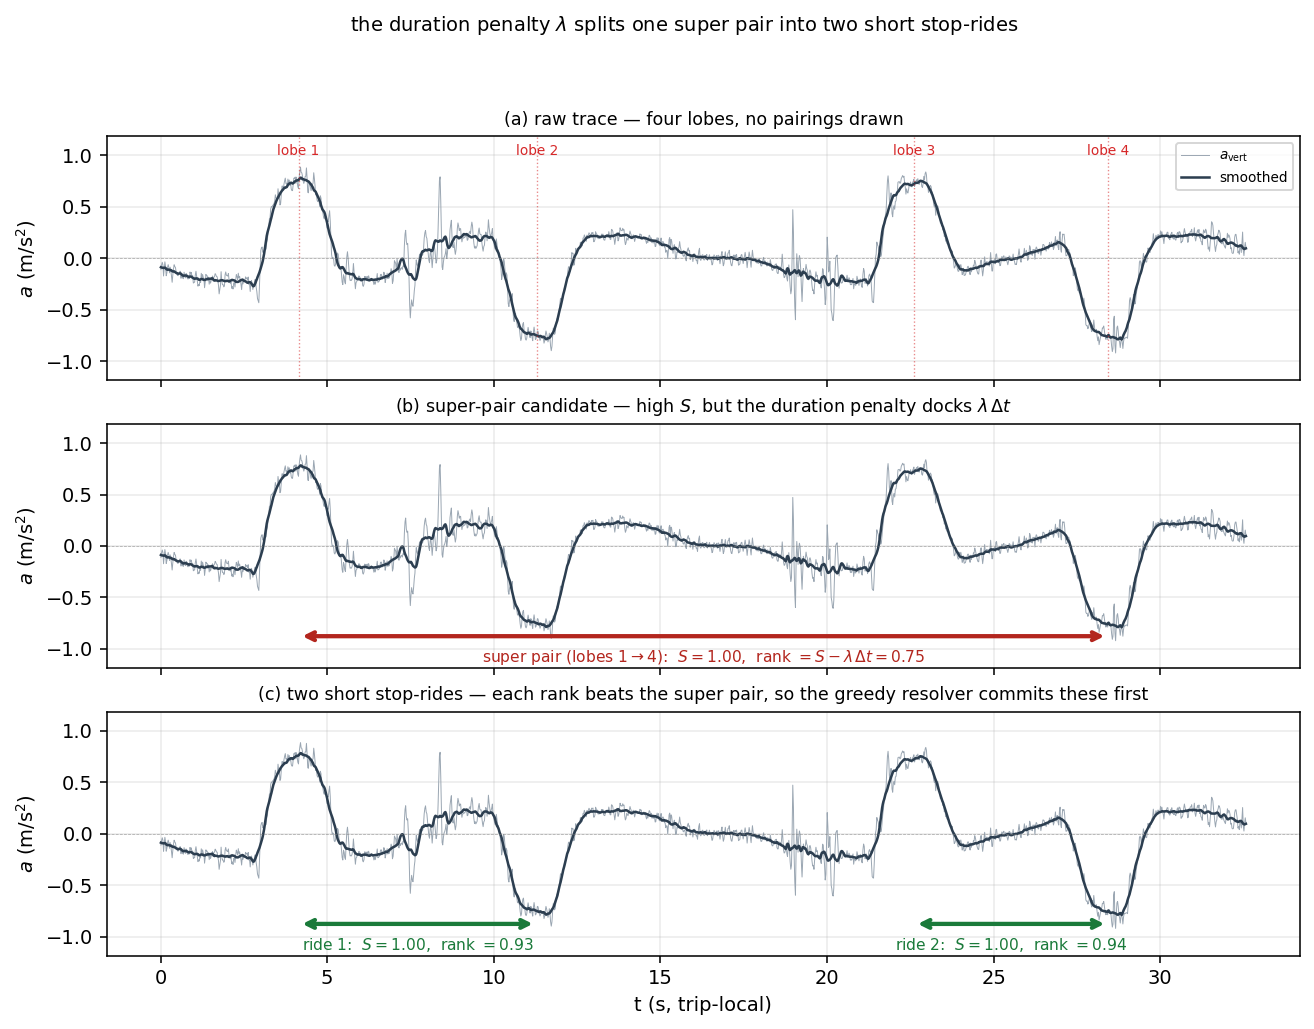
\includegraphics[width=\linewidth]{threshold_duration_penalty.png}
\caption{The duration penalty~$\lambda$ on an up-going multi-stop trip,
  reorganised into three panels.  \textbf{(a)}~The bare acceleration
  trace: four lobes, no pairings drawn.  \textbf{(b)}~The
  \emph{super-pair} candidate (red arrow): the take-off of the first
  ride paired with the landing of the last.  Its joint score~$S$ is
  high, but the rank~$S-\lambda\,\Delta t$ is docked by the wide span.
  \textbf{(c)}~The two short stop-rides (green arrows): each carries a
  comparable~$S$ but a far smaller~$\Delta t$, so each rank beats the
  super pair.  The greedy resolver commits the two short rides first,
  and the super pair never makes it onto the page of detected
  intervals.}
\label{fig:thresh-rank}
\end{figure}

\section{Prediction: error budget and conformal calibration}
\label{app:prediction}

This appendix derives the closed-form height~\eqref{eq:dh-closed},
the per-algorithm error budgets of~\S\ref{sec:algo-error}, and the
conformal coverage guarantee of~\eqref{eq:conformal-coverage}, and it
explains and illustrates every quality-filter check
of~\S\ref{sec:algo-quality}.

\subsection{The trapezoid pulse-pair integral}
\label{app:pred-integral}

The closed-form height~\eqref{eq:dh-closed} reduces to one
elementary scalar — the trapezoid area — used three times: once
per lobe and once for the cruise.

\paragraph{Lobe area.}
The trapezoid~$\tau_{W,f}$ of~\eqref{eq:trap-template} vanishes
outside~$[-W,W]$ and is a plateau of width~$2fW$ joined to zero by
two ramps of base~$(1-f)W$, so
\begin{equation}
  \int_{-\infty}^{\infty}\!\tau_{W,f}(t)\,dt
   \;=\;\underbrace{2fW}_{\text{plateau}}
        \;+\;\underbrace{2\cdot\tfrac12(1-f)W}_{\text{two ramps}}
   \;=\;W(1+f).
  \label{eq:trap-area}
\end{equation}
One lobe~$sA\,\tau_{W,f}$ therefore steps the cabin velocity
by~$v_{\mathrm{peak}}\!=\!A\,W(1+f)$: the take-off lobe carries the
cabin from rest to~$+v_{\mathrm{peak}}$, the landing lobe back to rest.

\paragraph{Displacement.}
The velocity~$v(t)$ rises through the take-off lobe, holds
at~$v_{\mathrm{peak}}$ across the inter-lobe cruise of
duration~$T_v\!=\!\Delta t_c\!-\!2W$, then falls through the landing
lobe (Figure~\ref{fig:trap-double-integral}).  The cruise contributes
$v_{\mathrm{peak}}\,T_v$ to~$\Delta h$.  Each ramp window contributes
$v_{\mathrm{peak}}\,W$: $\tau_{W,f}$ is symmetric about its centre, so
$v(t)$ is point-symmetric about each centroid
with~$v(t_{c,k})\!=\!v_{\mathrm{peak}}/2$, making its mean across the
$2W$-wide lobe window exactly~$v_{\mathrm{peak}}/2$.  Summing the
three slabs,
\[
  \Delta h \;=\; s\,v_{\mathrm{peak}}\,(2W+T_v)
            \;=\; s\,v_{\mathrm{peak}}\,\Delta t_c
            \;=\; s\,A\,W(1+f)\,\Delta t_c,
\]
which is~\eqref{eq:dh-closed}: the cruise velocity times the centroid
spacing, signed by the ride direction.

\begin{figure}[ht]
\centering
\resizebox{\linewidth}{!}{%
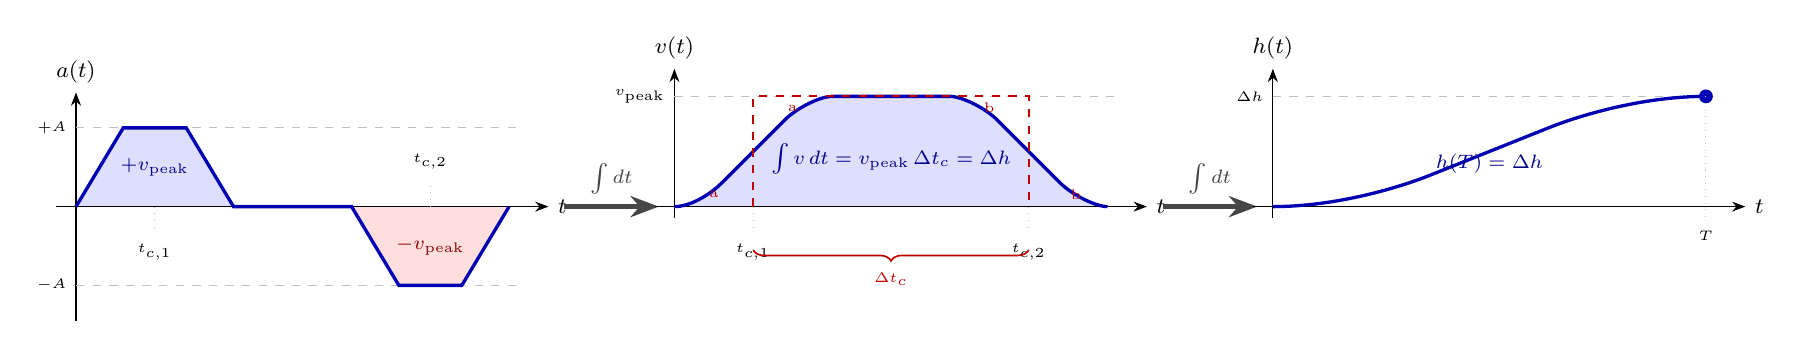
\begin{tikzpicture}[>=Stealth, font=\footnotesize]
  % Visual parameters: W=1, f=0.4, A=1, Tv=1.5 -> ride spans 0..5.5,
  % lobe centroids at t_{c,1}=1 and t_{c,2}=4.5, v_peak = AW(1+f) = 1.4,
  % Delta h = 4.9 (drawn rescaled to 1.4 for vertical-aspect parity).
  % ============= Panel 1: a(t) =============
  \begin{scope}[xshift=0cm]
    \fill[blue!13] (0,0) -- (0.6,1)  -- (1.4,1)  -- (2,0)   -- cycle;
    \fill[red!13]  (3.5,0) -- (4.1,-1) -- (4.9,-1) -- (5.5,0) -- cycle;
    \draw[->] (-0.25,0) -- (6.0,0) node[right] {$t$};
    \draw[->] (0,-1.45) -- (0,1.45) node[above] {$a(t)$};
    \draw[dashed,gray!50] (0,1)  -- (5.6,1);
    \draw[dashed,gray!50] (0,-1) -- (5.6,-1);
    \node[left,font=\tiny] at (0,1)  {$+A$};
    \node[left,font=\tiny] at (0,-1) {$-A$};
    \draw[very thick, blue!70!black]
      (0,0) -- (0.6,1)  -- (1.4,1)  -- (2,0)
            -- (3.5,0)
            -- (4.1,-1) -- (4.9,-1) -- (5.5,0);
    \node[blue!55!black] at (1.0, 0.5)  {\scriptsize $+v_{\mathrm{peak}}$};
    \node[red!55!black]  at (4.5,-0.5)  {\scriptsize $-v_{\mathrm{peak}}$};
    \draw[dotted,gray!55] (1,0)   -- (1,-0.32);
    \draw[dotted,gray!55] (4.5,0) -- (4.5,0.32);
    \node[below=1pt,font=\tiny] at (1,-0.32)  {$t_{c,1}$};
    \node[above=1pt,font=\tiny] at (4.5,0.32) {$t_{c,2}$};
  \end{scope}
  % --- arrow a -> v ---
  \draw[->, ultra thick, gray!55!black] (6.2,0) -- (7.4,0);
  \node[above=1pt, font=\scriptsize, gray!55!black] at (6.8,0) {$\int dt$};
  % ============= Panel 2: v(t) =============
  \begin{scope}[xshift=7.6cm]
    % shaded area under v(t)
    \fill[blue!13]
      (0,0) .. controls (0.2,0)    and (0.45,0.15) .. (0.6,0.3)
            -- (1.4,1.1)
            .. controls (1.55,1.25) and (1.85,1.4) .. (2.0,1.4)
            -- (3.5,1.4)
            .. controls (3.65,1.4) and (3.95,1.25).. (4.1,1.1)
            -- (4.9,0.3)
            .. controls (5.05,0.15) and (5.35,0)  .. (5.5,0)
            -- cycle;
    \draw[->] (-0.25,0) -- (6.0,0) node[right] {$t$};
    \draw[->] (0,-0.15) -- (0,1.75) node[above] {$v(t)$};
    \draw[dashed,gray!50] (0,1.4) -- (5.6,1.4);
    \node[left,font=\tiny] at (0,1.4) {$v_{\mathrm{peak}}$};
    \draw[very thick, blue!70!black]
      (0,0) .. controls (0.2,0)    and (0.45,0.15) .. (0.6,0.3)
            -- (1.4,1.1)
            .. controls (1.55,1.25) and (1.85,1.4) .. (2.0,1.4)
            -- (3.5,1.4)
            .. controls (3.65,1.4) and (3.95,1.25).. (4.1,1.1)
            -- (4.9,0.3)
            .. controls (5.05,0.15) and (5.35,0)  .. (5.5,0);
    % equivalent rectangle (v_peak high, Delta t_c wide, centroid to centroid)
    \draw[thick, red!75!black, dashed]
      (1,0) -- (1,1.4) -- (4.5,1.4) -- (4.5,0);
    % centroid ticks
    \draw[dotted,gray!55] (1,0)   -- (1,-0.32);
    \draw[dotted,gray!55] (4.5,0) -- (4.5,-0.32);
    \node[below=1pt,font=\tiny] at (1,-0.32)   {$t_{c,1}$};
    \node[below=1pt,font=\tiny] at (4.5,-0.32) {$t_{c,2}$};
    % Delta t_c brace
    \draw[decorate, decoration={brace,amplitude=4pt}, semithick, red!75!black]
      (4.5,-0.55) -- (1,-0.55);
    \node[below=2pt, font=\tiny, red!75!black] at (2.75,-0.65) {$\Delta t_c$};
    % integral label inside shaded area
    \node[blue!55!black, font=\scriptsize] at (2.75,0.6)
      {$\int v\,dt = v_{\mathrm{peak}}\,\Delta t_c = \Delta h$};
    % swap markers: light hatched pairs (left)
    \node[font=\tiny, red!70!black] at (0.5,0.15) {a};
    \node[font=\tiny, red!70!black] at (1.5,1.25) {a};
    % swap markers (right)
    \node[font=\tiny, red!70!black] at (5.1,0.15) {b};
    \node[font=\tiny, red!70!black] at (4.0,1.25) {b};
  \end{scope}
  % --- arrow v -> h ---
  \draw[->, ultra thick, gray!55!black] (13.8,0) -- (15.0,0);
  \node[above=1pt, font=\scriptsize, gray!55!black] at (14.4,0) {$\int dt$};
  % ============= Panel 3: h(t) =============
  \begin{scope}[xshift=15.2cm]
    \draw[->] (-0.25,0) -- (6.0,0) node[right] {$t$};
    \draw[->] (0,-0.15) -- (0,1.75) node[above] {$h(t)$};
    \draw[dashed,gray!50] (0,1.4) -- (5.6,1.4);
    \node[left,font=\tiny] at (0,1.4) {$\Delta h$};
    \draw[very thick, blue!70!black]
      (0,0)
      .. controls (0.8,0)    and (1.6,0.24) .. (2.0,0.4)
      -- (3.5,1.0)
      .. controls (3.9,1.16) and (4.7,1.4)  .. (5.5,1.4);
    \fill[blue!70!black] (5.5,1.4) circle (2.5pt);
    \draw[dotted, gray!55] (5.5,1.4) -- (5.5,-0.15);
    \node[below=1pt,font=\tiny] at (5.5,-0.15) {$T$};
    \node[blue!55!black, font=\scriptsize] at (2.75,0.55)
      {$h(T) = \Delta h$};
  \end{scope}
\end{tikzpicture}}
\caption{Double integration of the pulse pair.  Each acceleration
  lobe integrates to a velocity step of~$\pm v_{\mathrm{peak}}\!=\!\pm
  AW(1+f)$ centred at~$t_{c,1},t_{c,2}$; $v(t)$ holds at~$v_{\mathrm{peak}}$
  only on the inter-lobe cruise.  Each ramp window is
  point-symmetric about its centroid, so the shaded sliver
  outside the dashed rectangle~(\emph{a}, \emph{b}) has the same
  area as the unshaded sliver inside it, making the area
  beneath~$v(t)$ equal to~$v_{\mathrm{peak}}\,\Delta t_c\!=\!\Delta h$.}
\label{fig:trap-double-integral}
\end{figure}

In the short-ride limit~$\Delta t_c\!=\!2W$ the two lobes touch and
the cruise vanishes; \eqref{eq:dh-closed} collapses to the joined-pulse
height
\begin{equation}
  \Delta h \;=\; 2\,s\,A\,W^{2}(1+f),
  \label{eq:dh-joined}
\end{equation}
which the predictor fits as a three-parameter alternative on every
segment.

\subsection{ZUPT error budget}
\label{app:pred-zupt-error}

The ZUPT standard deviation~\eqref{eq:sigma-zupt-total} sums four
independent variances.

\paragraph{White-noise double integration.}
Integrating a white-noise acceleration sequence of per-sample
standard deviation~$\sigma_a$ once produces a velocity random walk;
integrating again produces a position.  After the linear drift term
of~\eqref{eq:zupt-integral} removes the unconstrained ramp mode, the
end-point position variance is $\sigma_a^{2}\,\Delta t^{4}\,N^{3}/12$
over~$N$ active samples, whose root is~\eqref{eq:sigma-zupt}.  The
cube in~$N$ is the double-integration random-walk scaling; the
factor~$1/12$ is the residual after the drift correction, against
the~$1/3$ of an uncorrected double integral.

\paragraph{Mechanical jitter.}
A hand-held phone is not a rigid inertial platform: hand tremor,
pocket friction, and skin-coupled breathing add a coloured-noise
acceleration band the datasheet omits.  The budget models it as an
extra acceleration~$\sigma_{\mathrm{mech}}^{a}
=j_0\,(1+\min(\rho/10^{\circ},2))$, a baseline
$j_0=0.03\,\mathrm{m/s^2}$ scaled up to threefold by the ride drift
angle~$\rho$, then integrated under ZUPT exactly as the white-noise
term: $\sigma_{\mathrm{mech}}
=\sigma_{\mathrm{mech}}^{a}\,\Delta t^{2}\sqrt{N^{3}/12}$.

\paragraph{Relative scale.}
The longer the ride, the larger the absolute error, because the
unmodelled coloured drift is roughly linear in the path integral of
acceleration.  A relative floor $\sigma_{\mathrm{rel}}
=k_{\mathrm{rel}}\,|\Delta h|$ with $k_{\mathrm{rel}}=0.05$ captures
it.

\paragraph{Projection penalty.}
A ride that lacks a clean stationary window projects its vertical
axis from a one-sided or in-ride gravity estimate, losing one or two
degrees of freedom on the vertical direction.  The penalty
$\sigma_{\mathrm{proj}}=(\pi-1)\cdot 0.25\,|\Delta h|$ scales with a
method factor $\pi\in\{1.0,1.2,1.3,3.0\}$ for the pre-and-post,
pre-only, post-only, and magnitude-only projections, further
multiplied by $1+\min(\rho_{\mathrm{pp}}/12.5^{\circ},2)$ for the
pre/post rotation angle~$\rho_{\mathrm{pp}}$.  Combined in
quadrature~\eqref{eq:sigma-zupt-total} and floored at~$0.15\,\mathrm{m}$,
the four terms give the per-ride standard deviation
\[
  \sigma_{\mathrm{ZUPT}}
  =\max\!\Big(
    \sqrt{\sigma_{\mathrm{white}}^{2}+\sigma_{\mathrm{mech}}^{2}
          +\sigma_{\mathrm{rel}}^{2}+\sigma_{\mathrm{proj}}^{2}},\;
    0.15\,\mathrm{m}\Big),
\]
so the conformal multiplier cannot blow up on a degenerate fit.

\subsection{Trapezoid error budget}
\label{app:pred-trap-error}

\paragraph{Matched-filter Cram\'er--Rao bound.}
Model the vertical trace as the fitted template pair plus Gaussian
noise of standard deviation~$\sigma_a^{\mathrm{eff}}$.  The Fisher
information of this likelihood bounds the variance of each fitted
parameter.  For the amplitude and the lobe centre,
\begin{equation}
  \sigma_A^{2}=\frac{(\sigma_a^{\mathrm{eff}})^{2}}{\langle\tau,\tau\rangle},
  \qquad
  \sigma_{t_c}^{2}
   =\frac{(\sigma_a^{\mathrm{eff}})^{2}}{A^{2}\,\langle\dot\tau,\dot\tau\rangle},
  \qquad
  \sigma_{\Delta t_c}^{2}=2\,\sigma_{t_c}^{2},
  \label{eq:crb}
\end{equation}
where $\langle\tau,\tau\rangle$ is the template energy
of~\eqref{eq:matched-filter} and
$\langle\dot\tau,\dot\tau\rangle=2/[(1-f)W]$ is the slope energy of
the two ramps.  A wider, sharper-edged lobe carries more energy and
more slope, so it pins both amplitude and timing more tightly.  The
grid quantises the shape parameters, so their variance is that of a
uniform prior over one grid cell, $\sigma_W^{2}=\Delta_W^{2}/12$ and
$\sigma_f^{2}=\Delta_f^{2}/12$.

\paragraph{Delta-method propagation.}
Differentiating the closed-form height~\eqref{eq:dh-closed} gives the
four gradients
\begin{equation}
  \frac{\partial\Delta h}{\partial A}=sW(1{+}f)\Delta t_c,\;\;
  \frac{\partial\Delta h}{\partial W}=sA(1{+}f)\Delta t_c,\;\;
  \frac{\partial\Delta h}{\partial f}=sAW\Delta t_c,\;\;
  \frac{\partial\Delta h}{\partial\Delta t_c}=sAW(1{+}f),
  \label{eq:dh-grad}
\end{equation}
and substituting~\eqref{eq:crb} and~\eqref{eq:dh-grad}
into the delta-method sum~\eqref{eq:sigma-dh} yields the per-segment
variance
\[
  \sigma_{\Delta h}^{2}
  =[W(1{+}f)\,\Delta t_c]^{2}\,\sigma_A^{2}
   +[A(1{+}f)\,\Delta t_c]^{2}\,\sigma_W^{2}
   +[AW\,\Delta t_c]^{2}\,\sigma_f^{2}
   +[AW(1{+}f)]^{2}\,\sigma_{\Delta t_c}^{2}.
\]

\paragraph{Data-adaptive effective noise.}
The white-noise figure from the sensor datasheet understates the
error on a hand-held phone by an order of magnitude.  The pipeline
replaces it with the residual root-mean-square of the fitted
template,
\[
  \sigma_a^{\mathrm{eff}}
  =\max\!\left(
    \sqrt{\tfrac1N\,\|a-\hat a_{\theta^{\star}}\|^{2}},\;
    \sigma_a^{\mathrm{ds}}\right),
\]
floored at the datasheet value~$\sigma_a^{\mathrm{ds}}$.  Whatever
the template fails to explain --- tremor, projection wobble, coloured
drift --- enters the residual, so the budget counts it automatically.
A second correction divides the effective variance by the fit
quality, $\tilde\sigma_a^{2}=(\sigma_a^{\mathrm{eff}})^{2}/
\max(R^{2}_{\mathrm{joint}},\varepsilon)$ with
$\varepsilon=10^{-3}$ --- the Wald post-regression form, in which a
poorly fitting template widens the posterior on every parameter in
proportion.

\paragraph{Velocity-anchored amplitude variance.}
When the fit of~\S\ref{sec:algo-trapezoid} replaces the
matched-filter amplitude with the measured cruise velocity, the
CRB~\eqref{eq:crb} no longer describes~$\sigma_A$.  The cruise
velocity is a mean of white-noise velocity samples, so
$\sigma_{\bar v}^{2}=\tilde\sigma_a^{2}\,\Delta t/T_{\mathrm{cruise}}$
and
$\sigma_{\widetilde A}^{2}=\sigma_{\bar v}^{2}/[W(1+f)]^{2}$, which
the pipeline substitutes for~$\sigma_A^{2}$ whenever the cruise
window is long enough to anchor ($T_{\mathrm{cruise}}>0.5$\,s).

\paragraph{Overlap inflation of the centroid spacing.}
The CRB~\eqref{eq:crb} treats the two lobe centres as independent.
At $\Delta t_c=2W$ the lobes touch but their supports stay disjoint,
the off-diagonal Fisher block is zero, and the diagonal CRB is exact.
For $\Delta t_c<2W$ --- unphysical for the shared-shape pair model ---
the two centre estimates correlate, and the budget inflates the
spacing variance by
\begin{equation}
  \sigma_{\Delta t_c}^{2}
   =2\,\sigma_{t_c}^{2}\left[\,1+
     \left(\frac{2W-\Delta t_c}{2W\,\delta}\right)^{2}\right],
   \qquad \delta=0.05,
  \label{eq:overlap-inflation}
\end{equation}
and the factor is~$1$ in the physical regime $\Delta t_c\ge2W$.  The
inflation keeps the budget well-conditioned without penalising a
genuine touching-lobe ride, which the joined-pulse
fit~\eqref{eq:dh-joined} handles directly.

\subsection{Split-conformal coverage and calibration}
\label{app:pred-conformal}

The multiplier~$k$ of~\S\ref{sec:algo-ci} is the
$\lceil(1-\alpha)(n+1)\rceil/n$ empirical quantile of the~$n$
calibration nonconformity scores~\eqref{eq:nonconformity}.  For
exchangeable rides the rank of a test score among the calibration
scores is uniform, so the test score falls at or below that quantile
with probability at least~$1-\alpha$ --- which
is~\eqref{eq:conformal-coverage}, with no assumption on the shape of
the error distribution.

The two algorithms calibrate~$k$ on different pools.  ZUPT calibrates
on every clean ride: the reported metrics are computed on clean data
regardless of the quality verdict, so a consumer who overrides the
filter still receives the promised coverage.  The trapezoid fit
calibrates on the rides that are both clean and quality-accepted ---
its exchangeable population, since a rejected trapezoid fit carries a
$\sigma$ the budget knowingly under-predicts.  Exchangeability fails
across the clean/corrupted split, so neither pool draws on corrupted
recordings.  The pipeline floors the multiplier at the Gaussian
$90\,\%$ half-width~$1.645$, and keeps an absolute floor and cap on
the reported~$k\sigma$ as a guard against a pathologically small or
large fitted~$\sigma$.

\subsection{Quality-filter checks}
\label{app:pred-quality}

Each algorithm runs its own quality
filter~(\S\ref{sec:algo-quality}).  The two filters share a shape:
hard gates that reject the ride outright at the first breach, and
graded score terms that sum into a penalty rejecting the ride
above~$6$.  Table~\ref{tab:quality-checks-zupt} lists the ZUPT checks;
Table~\ref{tab:quality-checks} the trapezoid checks.  The remainder of
this appendix walks each check one at a time: the real-world failure
it catches, the quantity it measures, and where the threshold comes
from.

\begin{table}[ht]
\centering
\small
\begin{tabular}{lll}
\toprule
\textbf{Check} & \textbf{Condition} & \textbf{Threshold} \\
\midrule
\multicolumn{3}{l}{\emph{Hard gates}}\\
Gravity calibration  & signed vertical projection available & reject if magnitude-only \\
Phone tilt           & $\angle(g_{\mathrm{pre}},g_{\mathrm{post}})\le$ & $25^{\circ}$ \\
Ride drift           & max gravity drift $\le$ & $15^{\circ}$ \\
Impact peak          & $\max|a-\bar a|\le$ & $8$\,m/s$^{2}$ \\
Active motion        & fraction $|a|>0.10\,\mathrm{m/s^2}\ge$ & $0.04$ \\
Displacement         & $|\widehat{\Delta h}|\in$ & $[0.4,100]$\,m \\
Segment length       & active samples $N\ge$ & $30$ \\
\midrule
\multicolumn{3}{l}{\emph{Score terms} (penalty sum rejects above $6$)}\\
Pre-window stability & $s_{\mathrm{pre}}$ & graded \\
Pre/post tilt        & $\angle(g_{\mathrm{pre}},g_{\mathrm{post}})$ & graded from $10^{\circ}$ \\
Ride drift           & max gravity drift & graded \\
Impact peak          & $\max|a-\bar a|$ & graded at $4,6$\,m/s$^{2}$ \\
End-velocity ratio   & $|v(T)|/\max|v|$ & graded \\
\bottomrule
\end{tabular}
\caption{ZUPT quality-filter checks and calibrated thresholds.}
\label{tab:quality-checks-zupt}
\end{table}

\begin{table}[ht]
\centering
\small
\begin{tabular}{lll}
\toprule
\textbf{Check} & \textbf{Condition} & \textbf{Threshold} \\
\midrule
\multicolumn{3}{l}{\emph{Hard gates}}\\
Gravity calibration  & signed vertical projection available & reject if magnitude-only \\
Phone tilt           & $\angle(g_{\mathrm{pre}},g_{\mathrm{post}})\le$ & $25^{\circ}$ \\
Joint $R^{2}$ floor  & $R^{2}_{\mathrm{joint}}\ge$ (short/mid/long) & $0.35/0.50/0.60$ \\
Displacement         & $|\widehat{\Delta h}|\in$ & $[0.4,120]$\,m \\
Lobe spacing         & $\Delta t_c\ge$ & $0.2$\,s \\
Active motion        & $(2W{+}\Delta t_c)/T_{\text{ride}}\ge$ & $0.05$ \\
Amplitude anchor     & $A_{\mathrm{used}}/A_{\mathrm{fit}}\in$ & $[0.5,2.0]$ \\
Out-of-lobe residual & residual density, outside/inside $\le$ & $4$ \\
Cruise steadiness    & $\mathrm{CV}(v_{\mathrm{cruise}})\le$ & $0.6$ \\
Segment length       & samples $N\ge$ & $30$ \\
\midrule
\multicolumn{3}{l}{\emph{Score terms} (penalty sum rejects above $6$)}\\
Pre-window stability & $s_{\mathrm{pre}}$ & graded \\
Pre/post tilt        & $\angle(g_{\mathrm{pre}},g_{\mathrm{post}})$ & graded from $10^{\circ}$ \\
Ride drift           & max gravity drift & graded \\
Joint $R^{2}$        & $R^{2}_{\mathrm{joint}}$ & graded below $0.8$ \\
Residual structure   & lag-1 residual ACF & graded at $0.25,0.4,0.6$ \\
\bottomrule
\end{tabular}
\caption{Trapezoid quality-filter checks and calibrated thresholds.
  The filter accepts a ride only when every hard gate passes and the
  penalty score stays below its cap.}
\label{tab:quality-checks}
\end{table}

\subsubsection*{Orientation checks (both filters)}

Every accelerometer estimate rides on a single vertical axis.  Three
checks defend that axis at three different time-scales: before the
ride, across the ride, and inside the ride.

\paragraph{Pre-window stationarity ($s_{\mathrm{pre}}$).}
The pipeline averages accelerometer samples in a rest window just
before the ride to recover the gravity direction.  A still phone
holds three flat axis traces; a swinging or rotating phone writes
wobble into all three, and the averaged vector then points wherever
the wobble happened to drift.  The filter measures the spread of
those gravity samples.  A window the filter cannot certify forces
the unsigned-magnitude fallback, and the filter rejects the ride.

\paragraph{Pre/post tilt.}
The pre/post tilt check repeats the rest-window trick after the ride
and compares the two gravity vectors.  Beyond $25^{\circ}$ the user
reoriented the phone mid-ride --- pulled it out of a pocket, handed
it off, flipped it on a table --- so no single projection serves both
ends.  Below $10^{\circ}$ the check is silent; between $10^{\circ}$
and the hard $25^{\circ}$ gate it adds a graded penalty.

\paragraph{Ride drift.}
Pre and post agreeing leaves a loophole: the phone can swing in the
middle and swing back.  Ride drift slices the ride into one-second
chunks and records the largest gravity angle relative to the
pre-window vector.  A held phone stays within a few degrees; an
actively handled one climbs past the $15^{\circ}$ gate, and the
vertical projection becomes ambiguous.

\subsubsection*{Motion-content checks (both filters)}

These checks reject segments where the algorithms have nothing useful
to fit.

\paragraph{Displacement bounds.}
Displacement bounds reject estimates outside the physically plausible
range.  Below $0.4\,\mathrm{m}$ is shorter than one stair step --- no
real elevator ride registers that small.  Above $100\,\mathrm{m}$ for
ZUPT or $120\,\mathrm{m}$ for the trapezoid fit is past the tallest
building in the campaign, so the estimate has run away.  Either
extreme rejects outright.

\paragraph{Active motion.}
The active-motion check rejects segments that carry almost no
acceleration signal.  ZUPT counts the fraction of samples
with~$|a|>0.10\,\mathrm{m/s^{2}}$ inside the segment and requires at
least $4\,\%$.  The trapezoid filter asks the equivalent question on
the fitted geometry: the two lobes plus the cruise gap together must
cover at least $5\,\%$ of the ride window.  Both hard gates fire only
on near-stationary phones, so in practice the graded score terms
carry the work.

\paragraph{Segment length.}
Segment length is a structural floor on the noise model.  Both error
budgets scale with the number of active samples~$N$, and below
$N=30$ sample-count variance dominates the per-ride~$\sigma$, so the
reported interval no longer reflects the noise model.  This floor is
geometric, not tuned.

\subsubsection*{ZUPT-only checks}

\paragraph{Impact peak.}
The impact-peak gate rejects rides where a non-elevator spike
dominates the trace.  ZUPT integrates acceleration twice, so any
spike feeds straight into~$\Delta h$.  A pocket drop, a tap, or a
hand-off easily clears $8\,\mathrm{m/s^{2}}$ --- ten times the
elevator's own lobes.  The gate rejects past $8\,\mathrm{m/s^{2}}$,
and the score grades the approach with knees at $4$ and
$6\,\mathrm{m/s^{2}}$.

\paragraph{End-velocity ratio.}
The end-velocity ratio scores how cleanly the ZUPT integrator
returned to rest.  A genuine ride starts and ends at zero velocity,
so $|v(T)|/\max|v|$ stays near zero on a healthy fit, and a large
ratio signals integrator drift the cruise plateau cannot absorb.
The magnitude-detrended trace pins the ratio near zero by
construction, so this check stays a graded score term, never a hard
gate.

\subsubsection*{Trapezoid fit-quality checks}

\paragraph{Joint $R^{2}$.}
The joint~$R^{2}$ floor measures how well the trapezoid template
explains the trace.  Short rides carry less acceleration energy and
have intrinsically worse signal-to-noise, so the floor scales with
predicted displacement: $0.35$ for short, $0.50$ for mid, $0.60$ for
long rides.  A fit below the matching floor never modelled the ride.

\paragraph{Residual autocorrelation.}
Residual autocorrelation catches what~$R^{2}$ misses: a template that
captures the lobe energy yet leaves a slow, structured bump in the
residual --- an unmodelled disturbance the squared-error sum cannot
see.  The lag-1 autocorrelation of the residual flags that structure.
Smoothing precedes the fit, so adjacent residuals are correlated by
construction even on a perfect ride; the score knees therefore sit
high, at $0.25$, $0.40$, and $0.60$.

\subsubsection*{Trapezoid fit-geometry checks}

\paragraph{Amplitude anchor ratio.}
The amplitude anchor ratio compares the two amplitudes the pipeline
produces for the same trapezoid: $A_{\mathrm{fit}}$ from the matched
filter and $A_{\mathrm{used}}$ from the integrated cruise velocity.
A trustworthy fit needs little rescaling between them, so a ratio
outside $[0.5,\,2.0]$ flags a template that locked onto the wrong
scale --- typically a matched-filter false positive with the wrong
$(W,f)$.

\paragraph{Out-of-lobe residual.}
Out-of-lobe residual density flags mid-ride disturbances the
trapezoid template missed.  A clean fit concentrates structure inside
the two lobe windows, so the residual energy density outside should
be no higher than inside.  A density ratio past fourfold means
something leaked energy into the cruise gap that the template never
modelled --- a passenger moving, a phone re-gripped, a multi-stop
trip miscounted as one ride.

\paragraph{Cruise steadiness.}
Cruise steadiness verifies the cabin reached constant velocity
between the two lobes.  The ZUPT-integrated velocity in that window
holds a flat plateau on a healthy ride.  A coefficient of variation
past $0.6$ means the plateau wobbled, so the cabin never settled
into steady cruise --- a short hop, a stop-go trip, or a misaligned
lobe pair.

\paragraph{Lobe spacing ($\Delta t_c$).}
Lobe spacing rejects pairs too close to be a take-off and a landing.
A centroid spacing below $0.2\,\mathrm{s}$ means the matched filter
paired two halves of the same lobe rather than two real lobes, so
the closed-form $\Delta h$ in~\eqref{eq:dh-closed} collapses to a
single-lobe area the model does not interpret.

\clearpage
\section{Evaluation: metrics and supporting figures}
\label{app:evaluation}

This appendix supplies the metric definitions and the diagnostic
figures behind the headline tables of~\S\ref{sec:evaluation}.

\subsection{Metric definitions}
\label{app:eval-metrics}

Every column of Tables~\ref{tab:eval-seg}, \ref{tab:eval-pred},
and~\ref{tab:eval-pipeline} comes from one of the metrics in
Table~\ref{tab:eval-metric-defs}.  Each row pairs the metric with
its physical meaning and with why the headline tables include it.

\begin{table}[H]
\centering
\small
\renewcommand{\arraystretch}{1.2}
\begin{tabular}{p{0.20\linewidth} p{0.36\linewidth} p{0.38\linewidth}}
\toprule
\textbf{Metric} & \textbf{Definition} & \textbf{Why we report it} \\
\midrule
$F1^{\ast}$ & Composite F1 over the four failure modes
  (\texttt{clean}, \texttt{missed}, \texttt{merged},
  \texttt{split}, FP); $\text{clean}/(\text{clean}+\frac12\,
  \text{bad}_{\rm GT}+\frac12\,\text{bad}_{\rm pred})$. &
  Distinguishes a miss-heavy configuration from a merge-heavy one;
  a pooled IoU-F1 averages the two. \\
IoU-F1@0.5 & PASCAL-style F1 at intersection-over-union $\ge 0.5$. &
  Comparable to any temporal-detection baseline; depressed by the
  GT pad of Figure~\ref{fig:eval-iou-pad}. \\
Median (m) & Median of $|\widehat{\Delta h}-\Delta h|$ over the
  ride set. & Robust scale of the bulk; the right read on
  ``typical'' per-ride accuracy. \\
MAE (m) & Mean of $|\widehat{\Delta h}-\Delta h|$. & Outlier-sensitive;
  the gap between median and MAE is the long-tail diagnostic. \\
$\le 1.5$\,m & Fraction of rides with absolute error $\le 1.5$\,m. &
  One-floor hit rate at the dataset's $\sim 3$\,m inter-floor pitch
  (\S\ref{app:dataset-buildings}) --- the right floor on either side. \\
$\le 3$\,m & Fraction of rides with absolute error $\le 3$\,m. &
  Two-floor hit rate; bounds the worst miss a downstream
  floor-detector still recovers. \\
Coverage & Fraction of rides with $|\widehat{\Delta h}-\Delta h|
  \le k\sigma$; nominal $90\,\%$. & Empirical check of the
  conformal guarantee~\eqref{eq:conformal-coverage}. \\
Median CI (m) & Median of $k\sigma$ across the ride set. &
  Typical interval width; the user's read on how tight a
  ``$90\,\%$ CI'' actually is. \\
Accept rate & Fraction of predictions the quality filter passes. &
  Recall trade-off of the filter; complements the per-ride scores. \\
\bottomrule
\end{tabular}
\caption{Every metric used in the headline evaluation tables, with
  the definition and the reason the contract needs it.  Coverage
  and Median CI together carry the calibrated-interval promise of
  \S\ref{sec:intro}; the $\le 1.5$\,m and $\le 3$\,m columns
  translate that promise into the floor-detection unit the
  downstream consumer uses.}
\label{tab:eval-metric-defs}
\end{table}

\subsection{Segmentation supporting figures}
\label{app:eval-extra-seg}

Figure~\ref{fig:eval-seg-failures} disaggregates
Table~\ref{tab:eval-seg} into its five failure categories.  The
\texttt{clean} bar dominates both splits; the \texttt{missed} and
\texttt{FP} tails are shorter on the held-out test than on the
tuned train pool.

\begin{figure}[H]
\centering
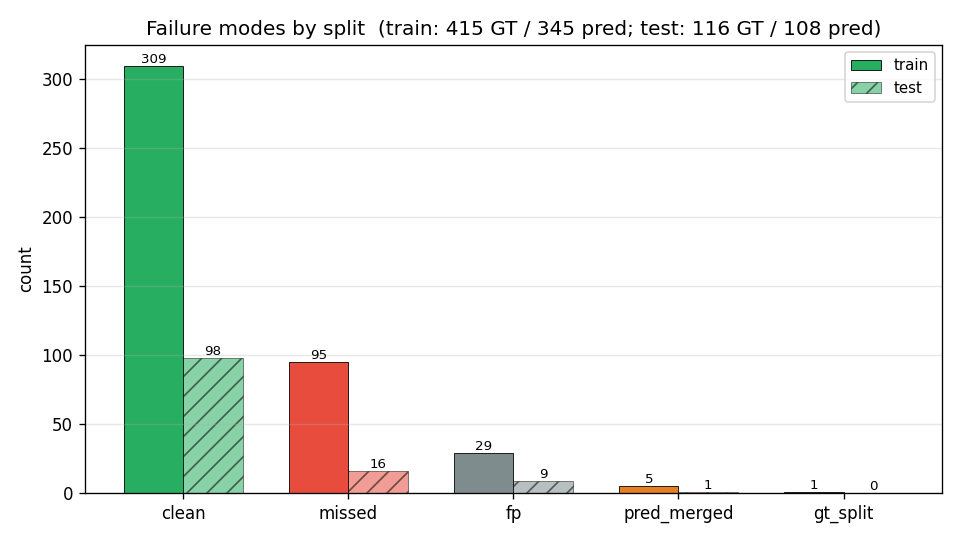
\includegraphics[width=0.65\linewidth]{seg_failure_modes.png}
\caption{Segmentation failure-mode counts on the train pool (solid)
  and the held-out test building (hatched), normalised by GT ride
  count.  The bulk of the train pool's $95$ missed rides comes
  from three heavily damped Pixel\,10 sessions where the
  matched-filter amplitude floor swallows the lobes
  (\S\ref{sec:discussion}); the held-out building carries no such
  session, driving the test-set lift on $F1^{\ast}$.}
\label{fig:eval-seg-failures}
\end{figure}

\subsection{Per-ride prediction supporting figures}
\label{app:eval-extra-pred}

Two diagnostics anchor Table~\ref{tab:eval-pred}: the empirical
CDF that produces the $\le 1.5$\,m and $\le 3$\,m columns, and the
signed-error PDF that checks for bias.

\paragraph{Error CDF.}
Figure~\ref{fig:eval-pred-cdf} plots the cumulative distribution
of $|\widehat{\Delta h}-\Delta h|$ for the trapezoid fit across the
pooled clean rides.  The $\le 1.5$\,m and $\le 3$\,m fractions of
Table~\ref{tab:eval-pred} are the $y$-values where the curve
crosses the two vertical lines.

\begin{figure}[H]
\centering
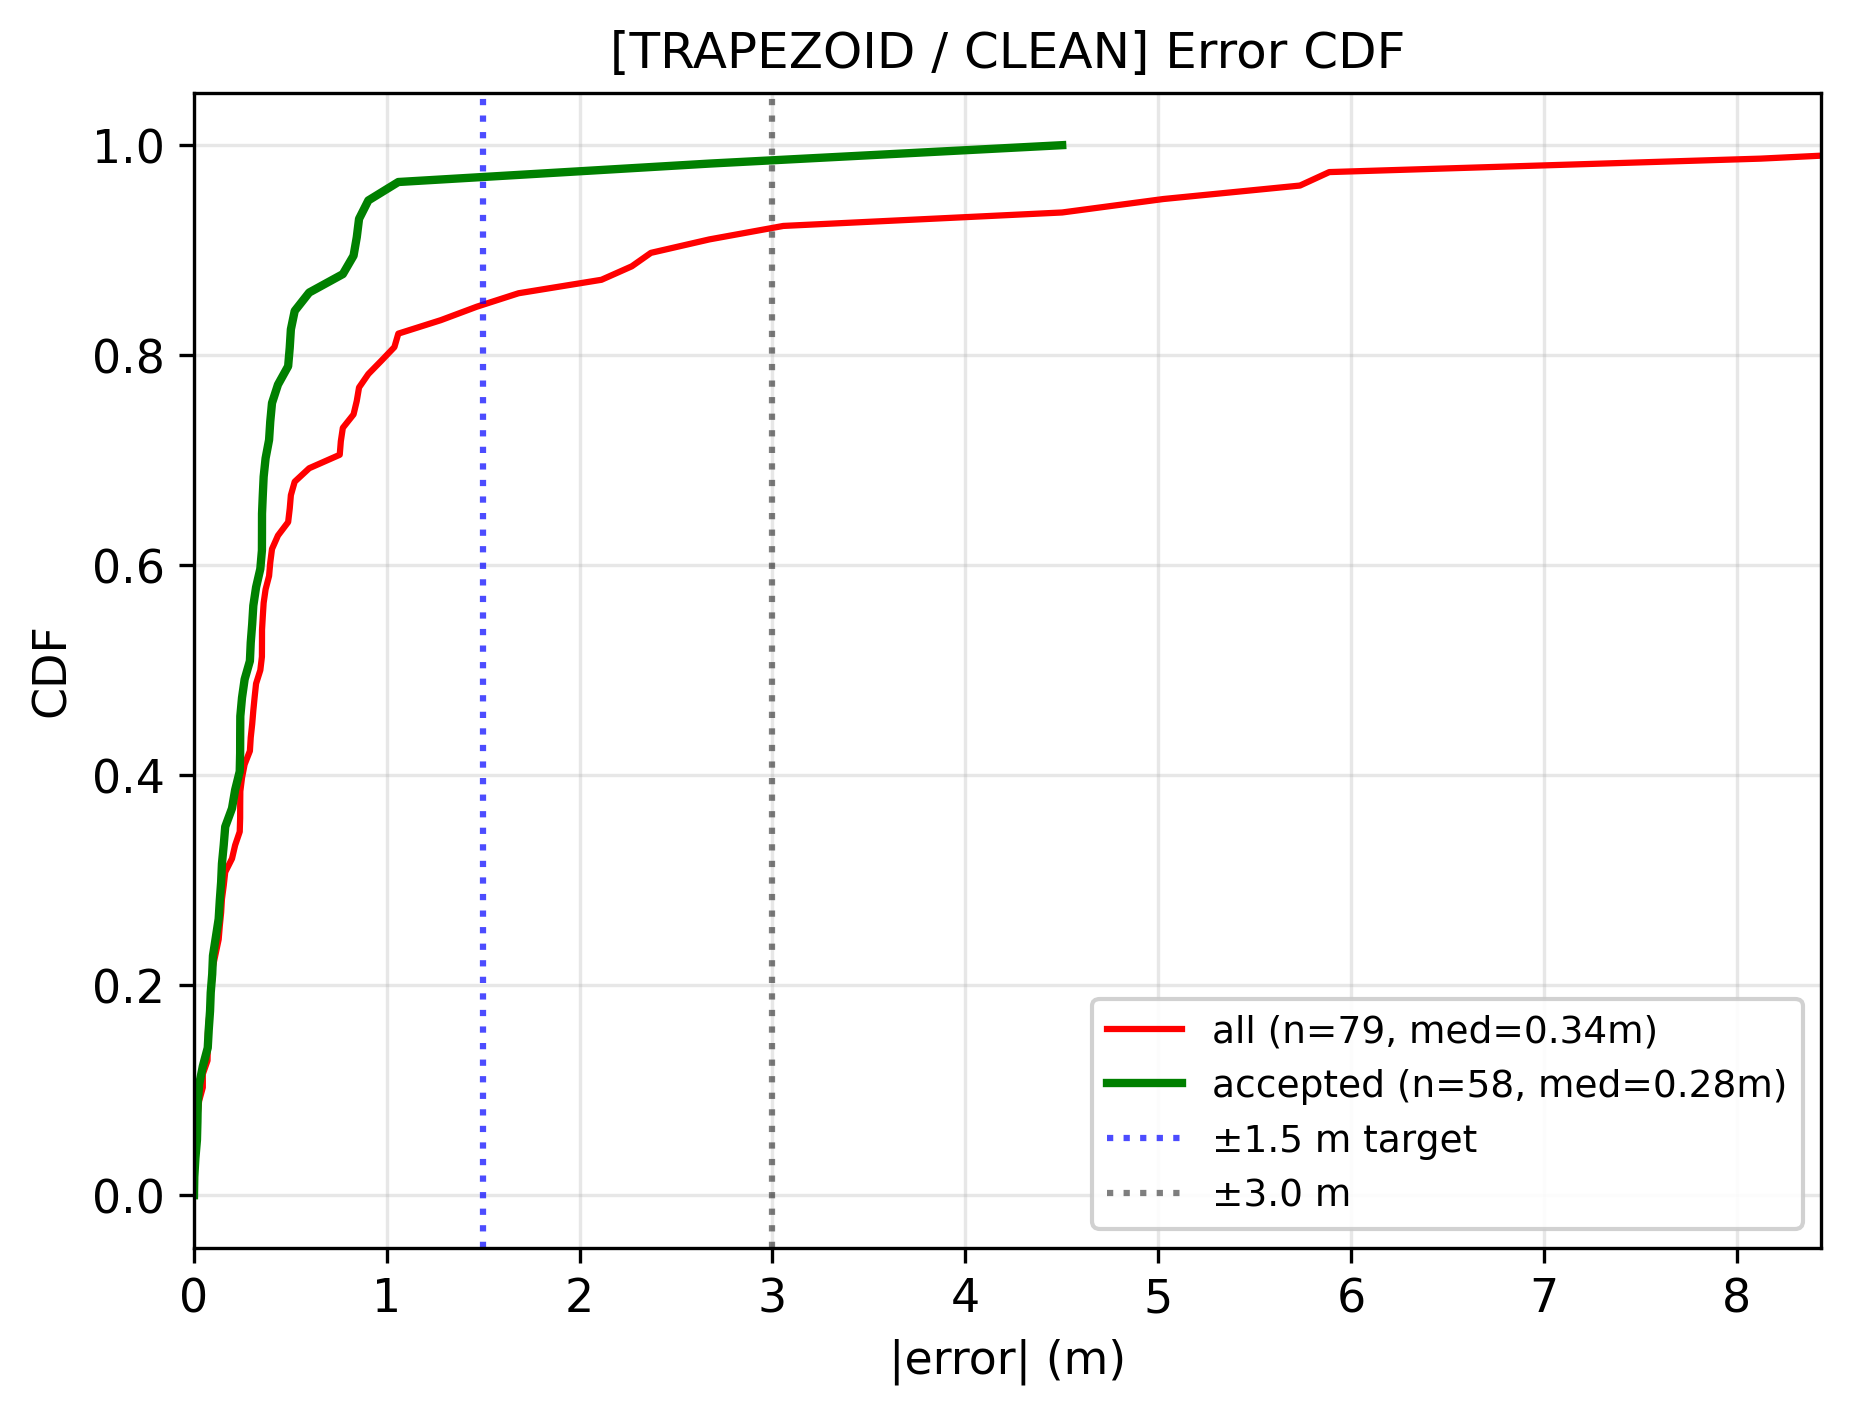
\includegraphics[width=0.65\linewidth]{pred_cdf.png}
\caption{Empirical CDF of absolute $\Delta h$ error for the
  trapezoid fit on clean rides.  Vertical dashed lines mark the
  $\pm 1.5$\,m and $\pm 3$\,m floor targets; the curve crosses
  $\pm 1.5$\,m by roughly the $88\,\%$ percentile and
  $\pm 3$\,m by the $93\,\%$ percentile.}
\label{fig:eval-pred-cdf}
\end{figure}

\paragraph{Signed-error distribution.}
The signed-error PDF (Figure~\ref{fig:eval-pred-signed}) checks
that the predictor is not systematically biased upward or
downward.  A symmetric, zero-centred PDF means the fit's bias is
small compared to its variance; any drift in the mean would
otherwise corrupt the calibrated interval of~\S\ref{sec:algo-ci}.

\begin{figure}[H]
\centering
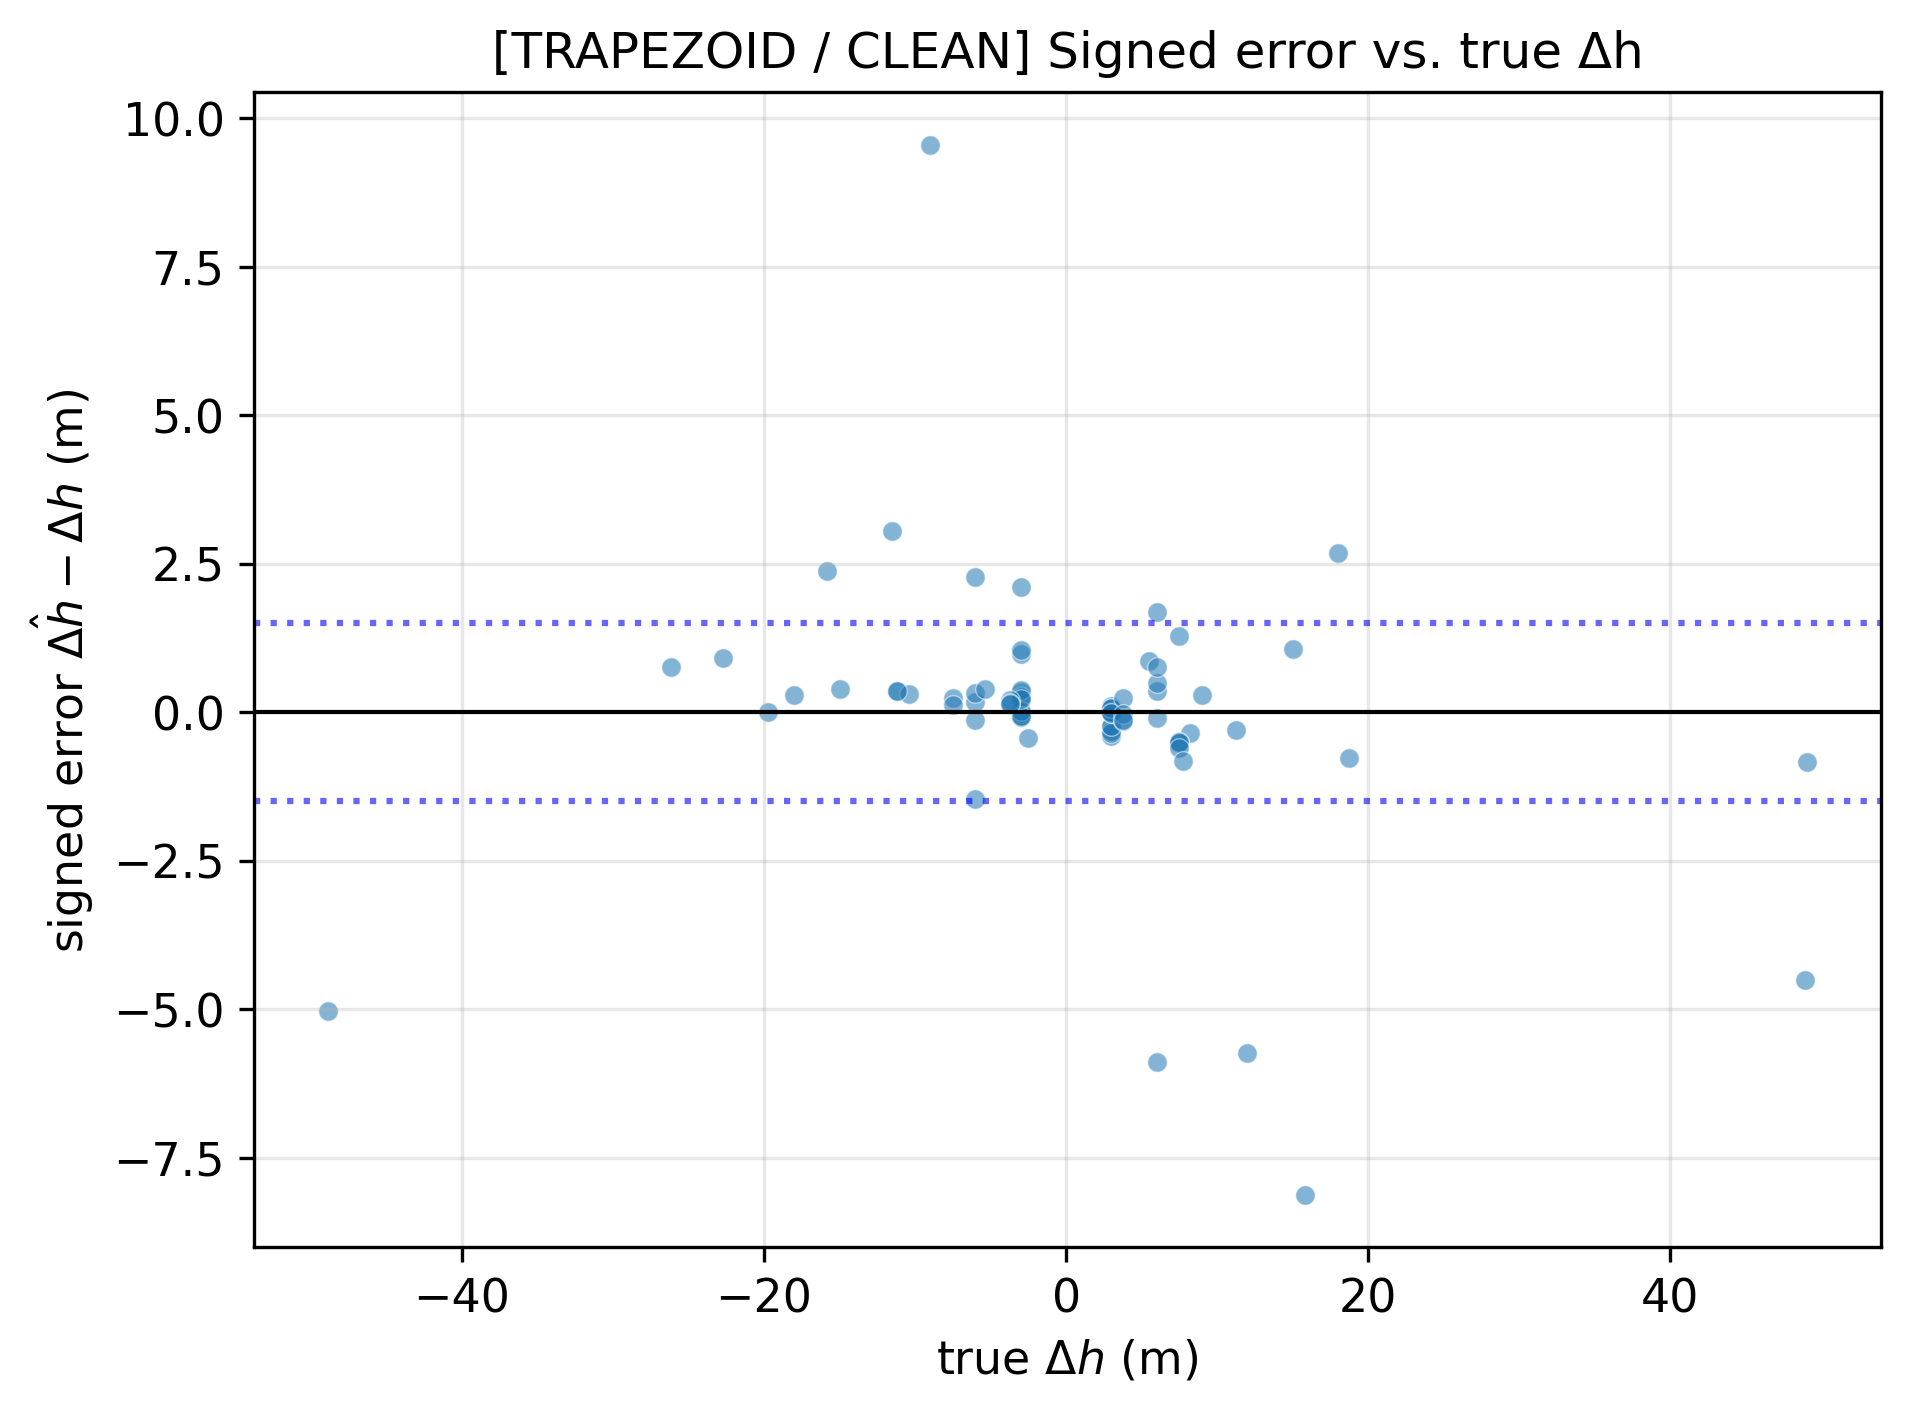
\includegraphics[width=0.65\linewidth]{pred_signed_err.png}
\caption{Density of signed error $\widehat{\Delta h}-\Delta h$ on
  pooled clean trapezoid rides.  The PDF is centred near zero;
  the tails are heavier than Gaussian, which is why the
  distribution-free conformal interval of~\eqref{eq:conformal-coverage}
  is the right calibration tool rather than a $1.645\,\sigma$
  Gaussian quantile.}
\label{fig:eval-pred-signed}
\end{figure}

\paragraph{Per-view scatter.}
Figure~\ref{fig:eval-pred-scatter-three} stitches the trapezoid
fit, the matched-segmenter view, and the all-segments-versus-
barometer view onto one panel each.  The off-diagonal tail in the
right panel is the false-positive cost the quality filter
of~\S\ref{sec:eval-pipeline} removes.

\begin{figure}[H]
\centering
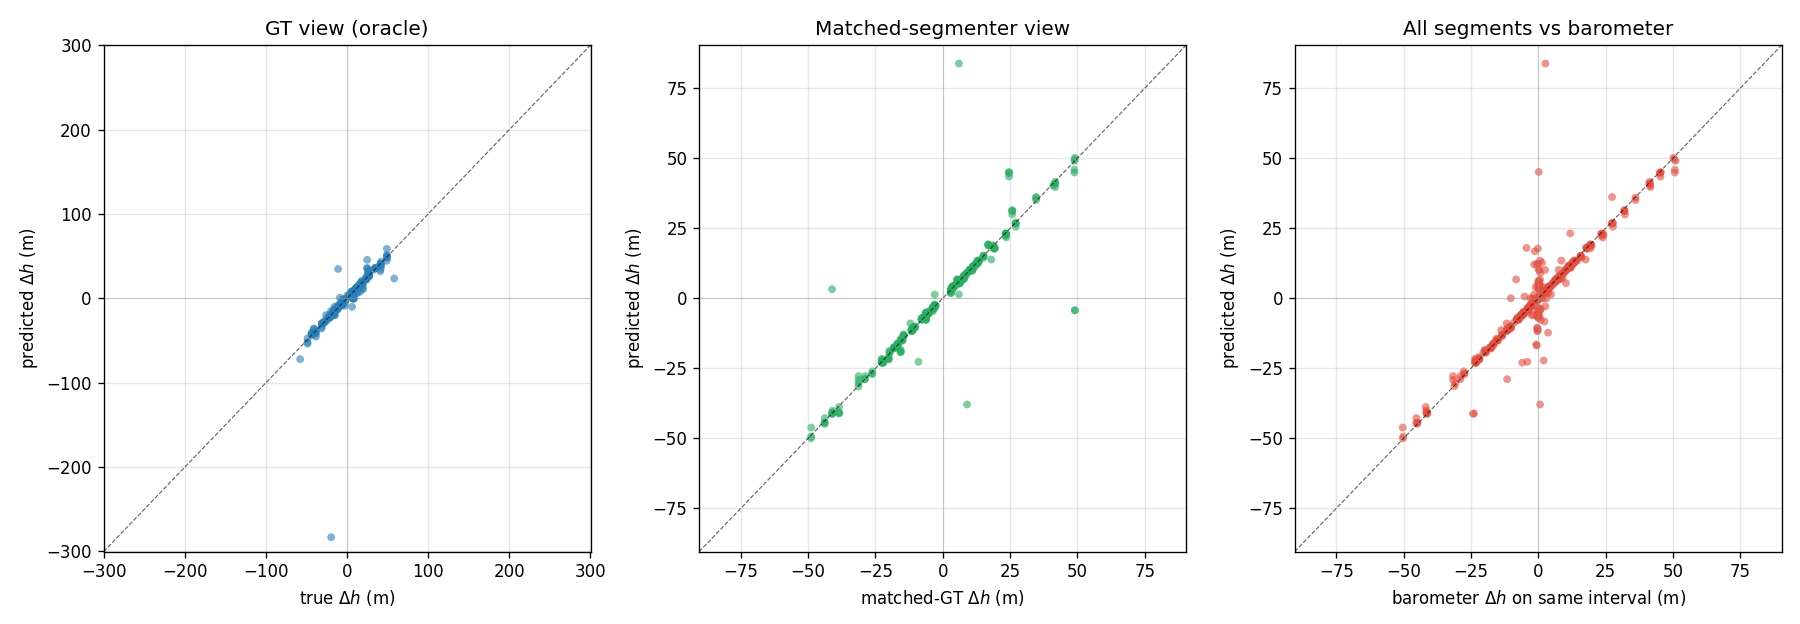
\includegraphics[width=0.95\linewidth]{pred_scatter.png}
\caption{Predicted versus ground-truth $\Delta h$ on every clean
  ride, one panel per evaluation view: GT-segments (predictor on
  every GT interval, left), matched-segmenter (predictor on
  segmenter intervals that cleanly match a GT, middle), and
  all-segments-versus-barometer (predictor on every segmenter
  interval scored against the barometer, right).  Mean error in
  Table~\ref{tab:eval-pred} is driven by the far-from-diagonal
  points, where double integration of a body-frame trace
  accumulates drift on the damped recordings.}
\label{fig:eval-pred-scatter-three}
\end{figure}

\subsection{Pipeline supporting figures}
\label{app:eval-extra-pipeline}

Figure~\ref{fig:eval-pipeline-cdf} shows the deployed pipeline's
accepted-only CDF: the same axis as Figure~\ref{fig:eval-pred-cdf}
after the quality filter is in the loop.  Every view crosses the
$\pm 1.5$\,m floor target before the $90$th percentile.

\begin{figure}[H]
\centering
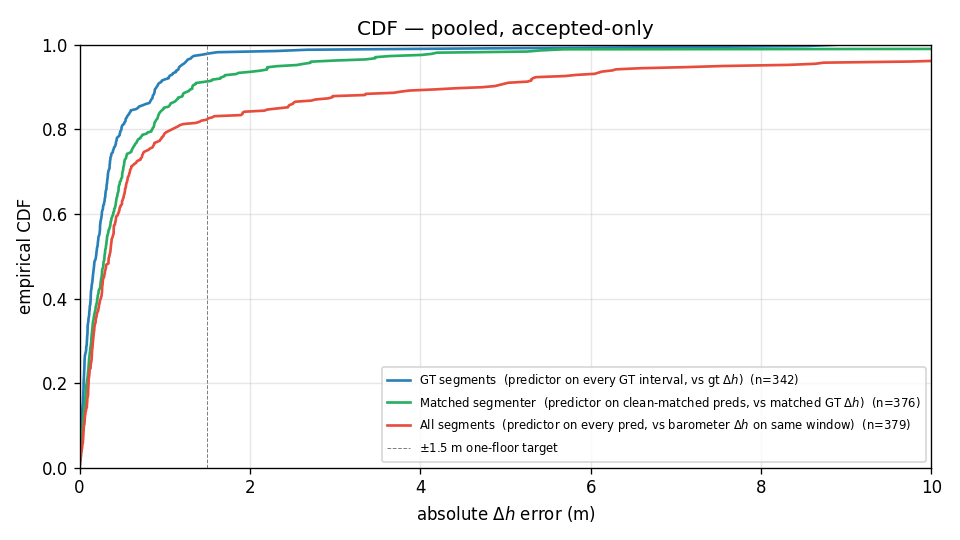
\includegraphics[width=0.65\linewidth]{pipeline_cdf_acc.png}
\caption{Empirical CDF of absolute $\Delta h$ error on the
  deployed pipeline (accepted-only), pooled across both splits and
  broken into the three evaluation views of
  Figure~\ref{fig:eval-pred-scatter-three}.  The trade-off the
  filter introduces is recall: $18\,\%$ of clean trapezoid rides
  and $7\,\%$ of clean ZUPT rides are rejected, so a downstream
  consumer sees about four out of every five real rides --- each
  flagged with a coverage-guaranteed interval.}
\label{fig:eval-pipeline-cdf}
\end{figure}

\end{document}
